\documentclass[12pt,a4paper,oneside,norsk]{article} 
\usepackage[utf8]{inputenc}
%\usepackage[norsk]{babel}
\usepackage{amsmath}
\usepackage{amsfonts}
\usepackage{amssymb}
\usepackage{makeidx}
\usepackage{graphicx}
\usepackage{hyperref}
\usepackage[left=2cm,right=2cm,top=2cm,bottom=2cm]{geometry}
\usepackage{float}
\usepackage{multirow}
\usepackage{verbatim} %for å kommentere ut ting
\usepackage[nottoc,numbib]{tocbibind}
\usepackage{chngpage} % allows for temporary adjustment of side margins
\usepackage[parfill]{parskip} %for avsnitt
\usepackage[yyyymmdd,hhmmss]{datetime}
\usepackage{comment} 
\usepackage{caption}
\captionsetup[figure]{labelformat=empty}

\raggedbottom

\usepackage{makeidx}
\makeindex

\begin{document}
%her kommer forsiden:
    \begin{titlepage}
    \begin{center}
    \ \\
    \ \\
    \ \\
    The Gentleman's Club \\
    \ \\
    \ \\
    \ \\
    \ \\
    \ \\
    \ \\{\large \bfseries
    The Gentleman's Club Official Alcoholic Beverages Chart\\
    }
    \ \\
    \ \\
\begin{figure} [H]
\centering
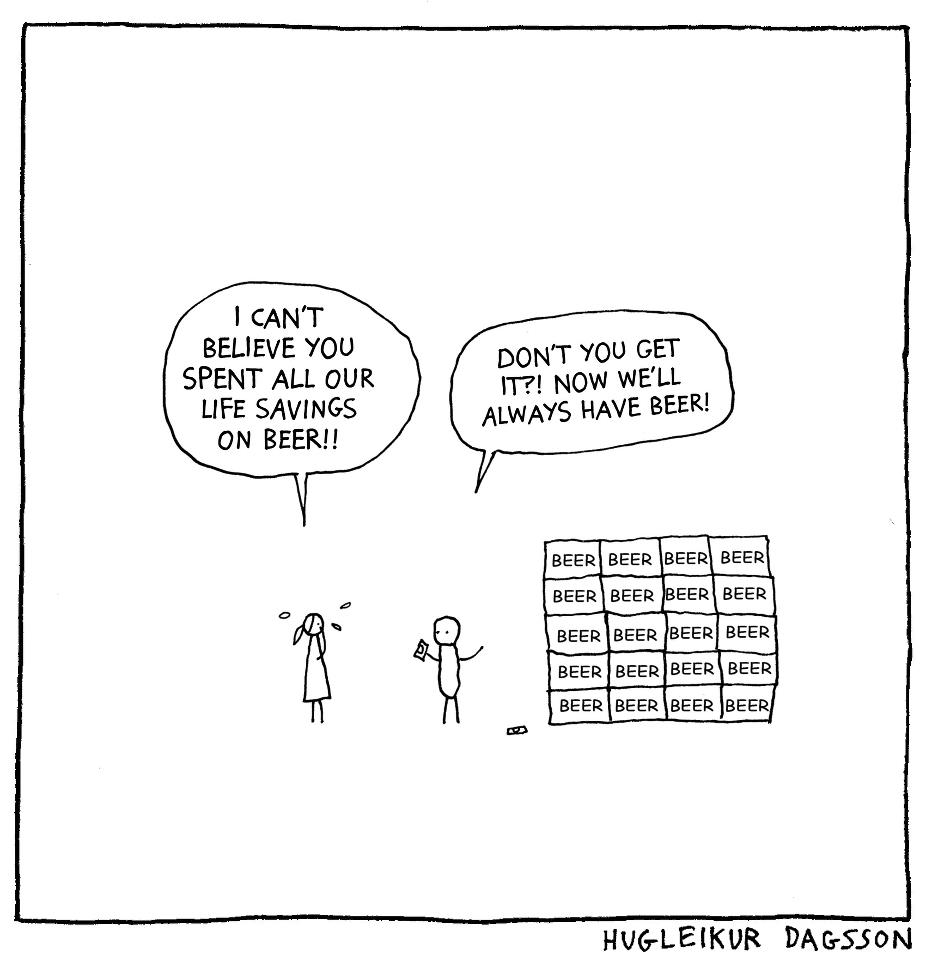
\includegraphics[scale=0.45]{Bilder/forside.jpg} %scale justerer størrelsen på bilde. Linjen etterpå er mappen bilde ligger i.
\end{figure}
    \ \\
    \ \\
        {\large
    Alcoholic Beverages Chart\\
    }
    \ \\
    {\today\ \\}
    \ \\
    \end{center}
    \end{titlepage}
    
    \thispagestyle{empty}
\newpage

\setcounter{page}{1}
\pagenumbering{arabic}
%her er innholdsfortegnelsen. Den lages automagisk
\tableofcontents
\newpage

%HER ER EN LITEN BRUKSANVISNING
%Nedenfor er en mal til hvordan man lager en subsubsection
\begin{comment}
%start å klipp og lim herifra, og lim det inn under riktig "subsection":

\subsubsection{Bryggeri: NAVN PÅ ØL}
\paragraph{Kommentar:} SKRIV DIN MENING HER
\newline
-- -- ( SKRIV NAVN OG DATO)

\begin{figure} [H] %[H] hindrer latex i å bestemme hvor bilde skal stå. men det kommer der du vil ha det.
\centering
\includegraphics[scale=0.60, angle=0]{Bilder/Ol/outcomeinterruption.png} %scale justerer størrelsen på bilde, angle rotasjonen. Linjen etterpå er mappen bilde ligger i.
\caption{SKRIV EN BILDE TEKST.}
\end{figure}
\newpage
%stopp med klipp og lim her! --------------------------
\end{comment}


\section{Øl}
\subsection{Bayer}

\subsubsection{Det Lille Bryggeriet: Bjønnøl}
\paragraph{Kommentar:}Kjedelig og smakløst øl. Lever ikke opp til navnet og er ikke verdt pengene.
\newline
-- -- Isak 13.04.2014

\begin{figure} [H]
\centering
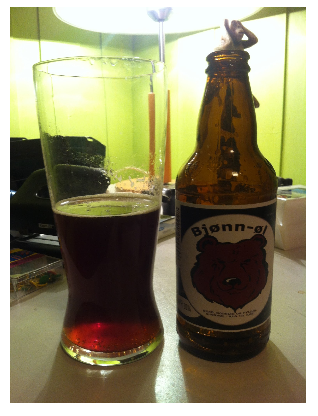
\includegraphics[scale=1.00]{Bilder/Ol/bjonnol.PNG} 
\caption{Bjønnøl fra "Det Lille Bryggeri"}
\end{figure}

\newpage
\subsection{Ale}

\subsubsection{Nøgne Ø: Red Horizon }
\paragraph{Kommentar:} Dette var en svin god øl, veldig sammensatt og komplisert smak. På mange måter minnet den litt mer om vin enn øl. Igjen var den kanskje litt søt for min smak, men denne var likevel så god at jeg ikke har noe å utsette på den. Jeg vil absolutt anbefale en flaske. Kanskje ved siden av noe god mat, men jeg tror det kan være vanskelig å finne mat som ikke ødelegger hele smaksbildet dens. Uansett, dette er noe man må smake!
\newline
-- -- Anders 30.11.2014

\begin{figure} [H] 
\centering
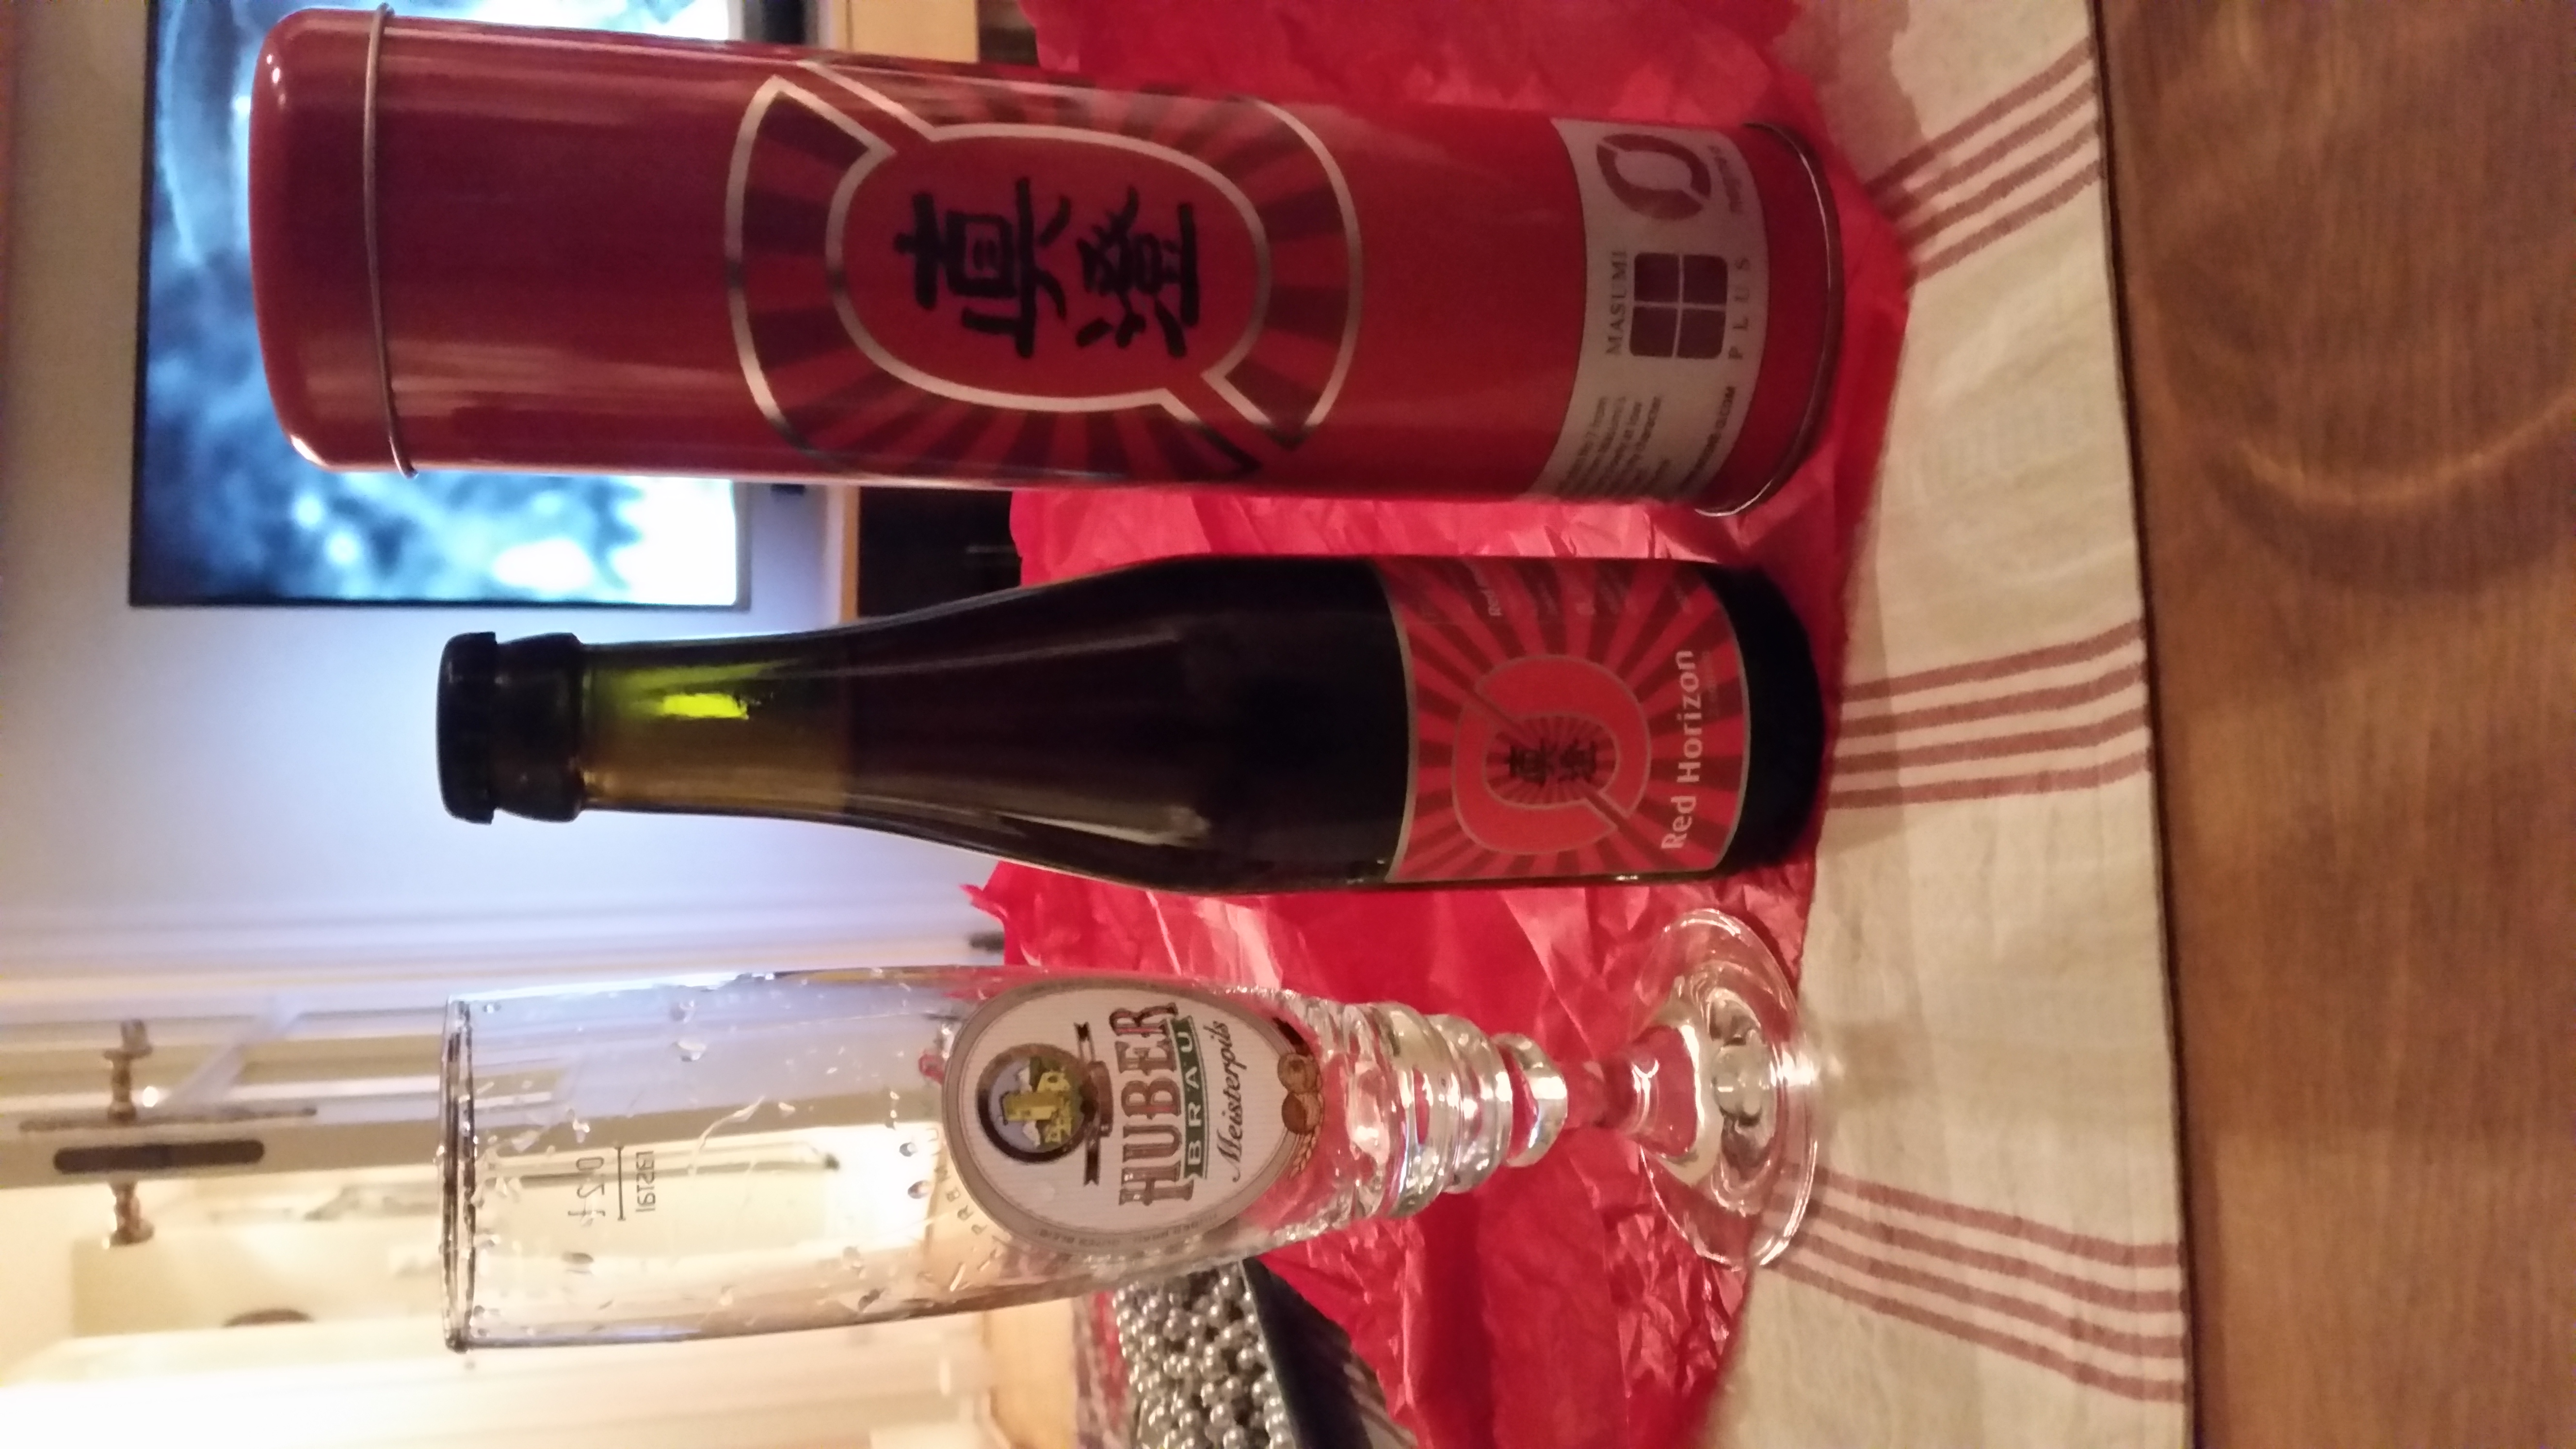
\includegraphics[scale=0.04, angle=-90]{Bilder/Ol/redHorizon.jpg}
\caption{Red Horizon fra Nøgne Ø.}
\end{figure}

\begin{figure} [H] 
\centering
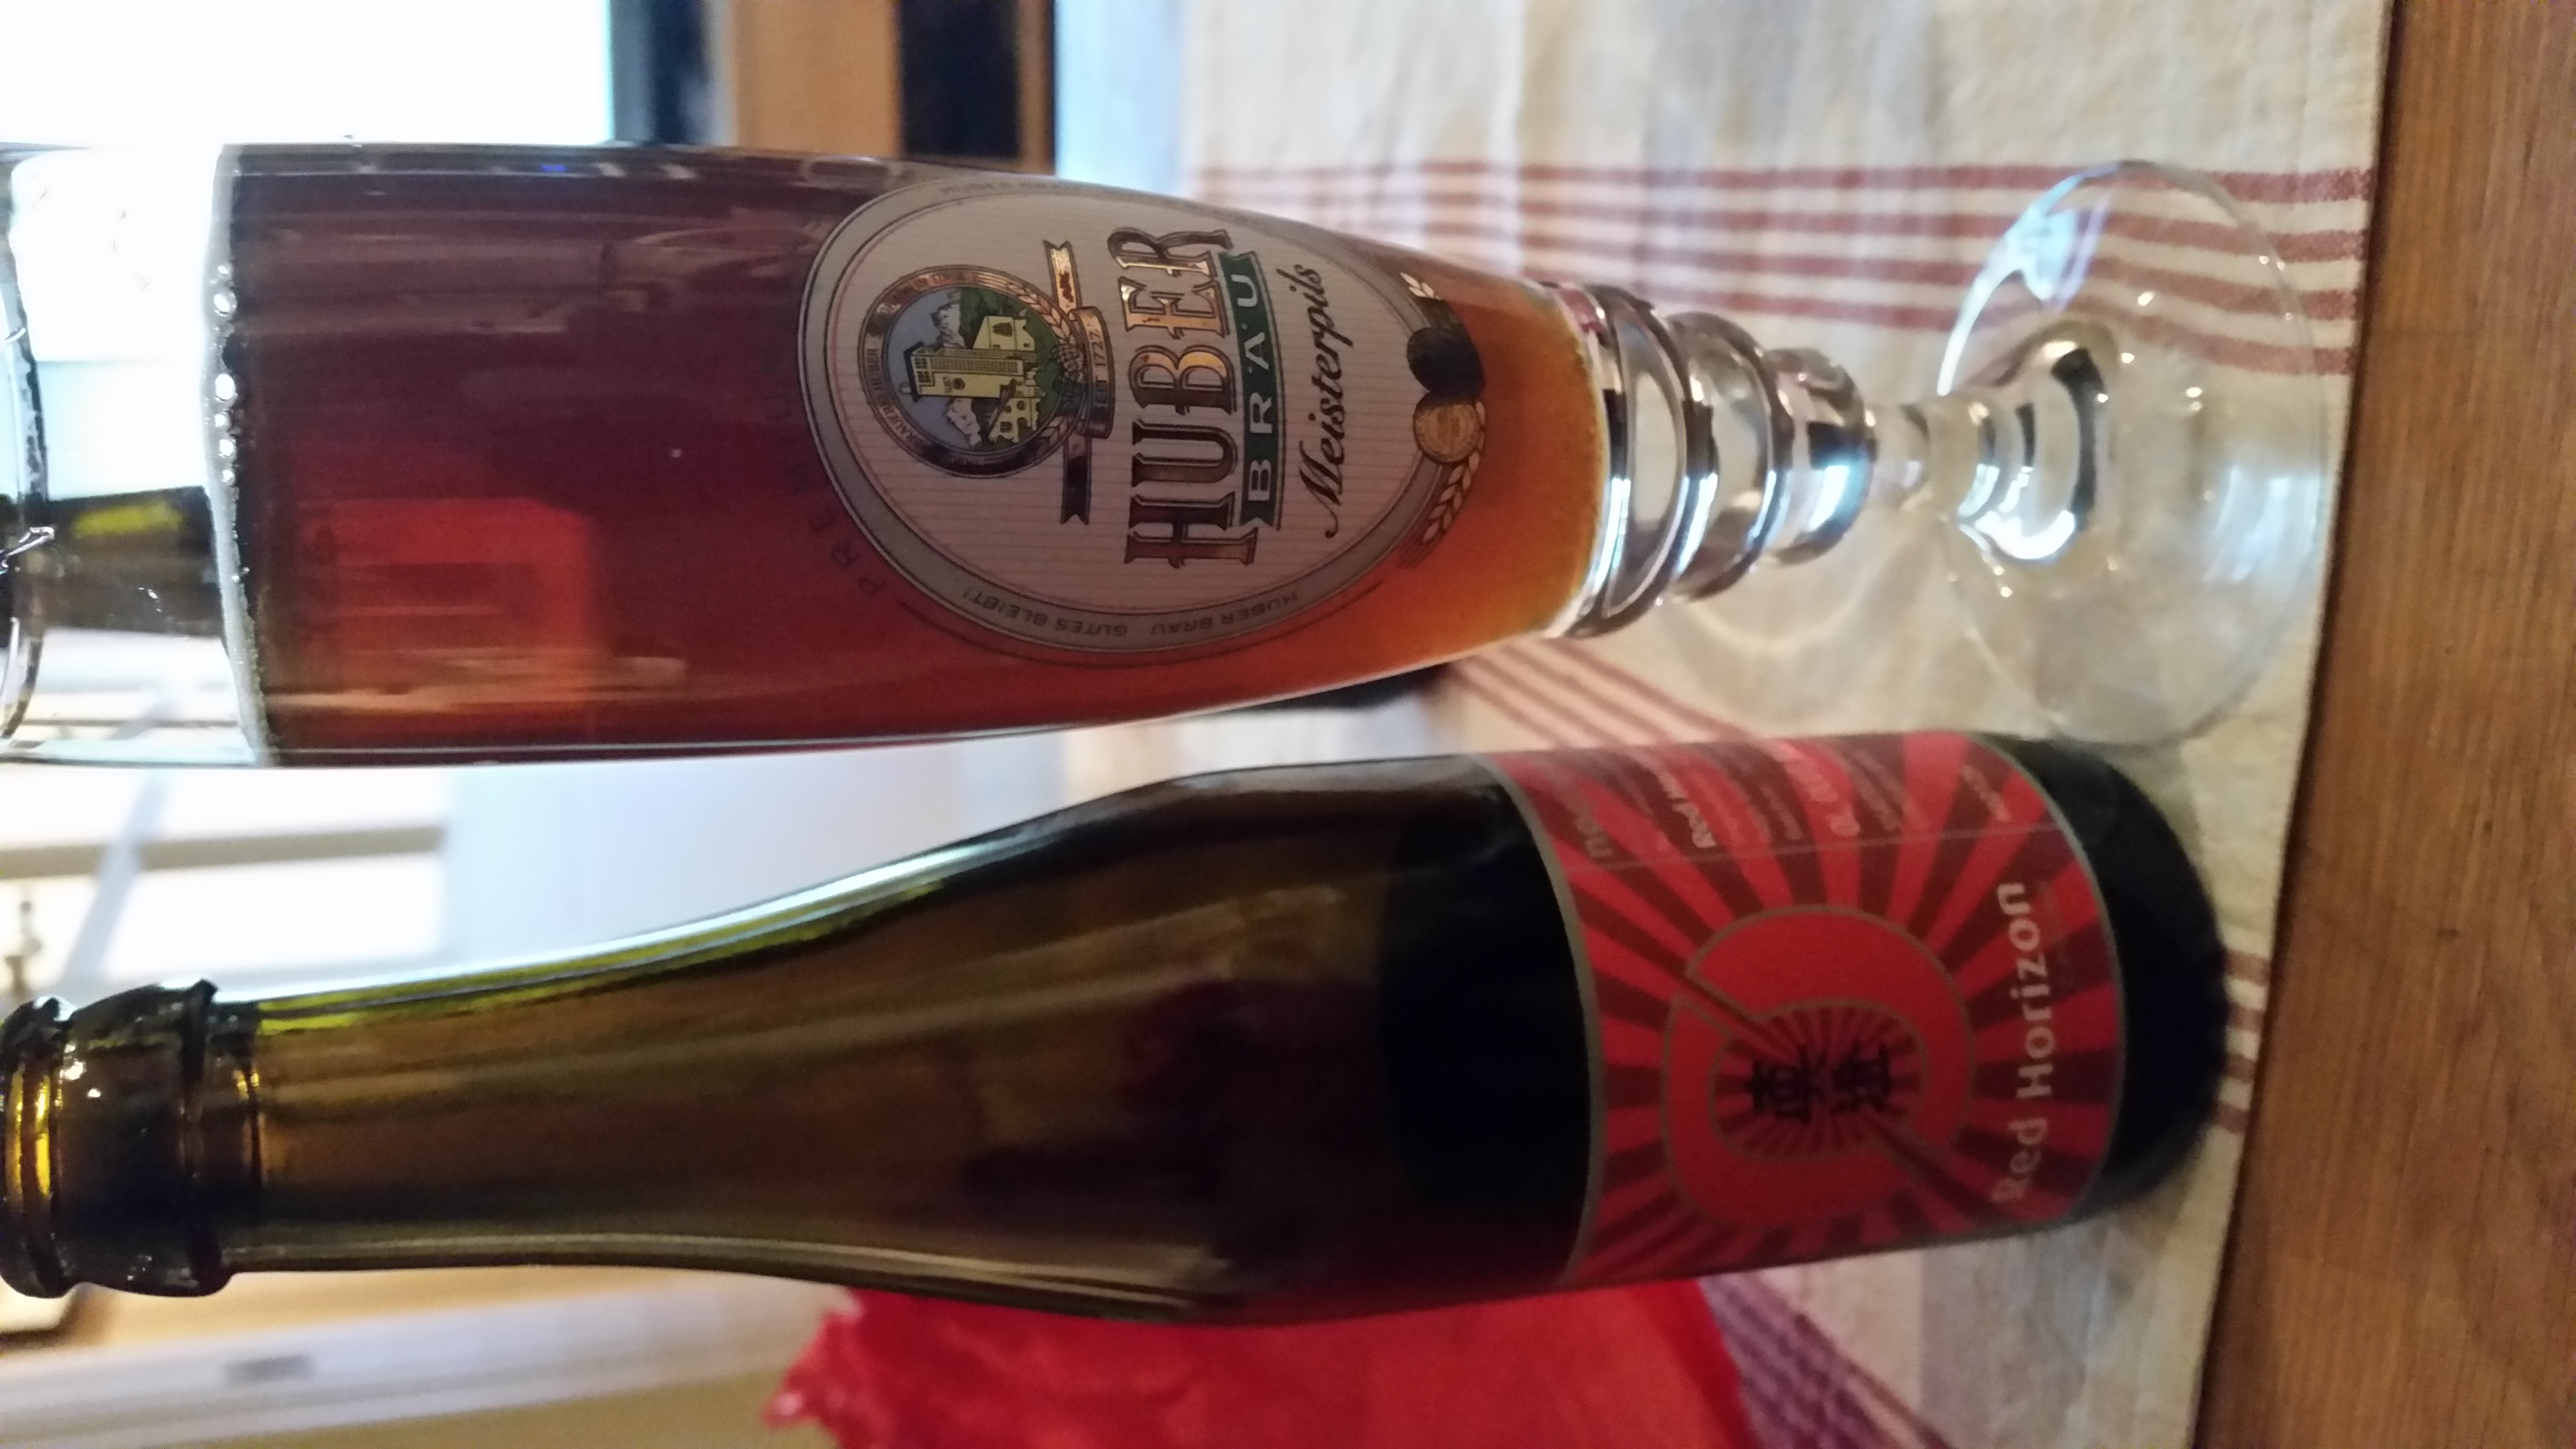
\includegraphics[scale=0.04, angle=-90]{Bilder/Ol/redHorizon1.jpg}
\caption{Red Horizon  fra Nøgne Ø.}
\end{figure}
\newpage

\subsubsection{Nøgne Ø: Sunturnbrew}
\paragraph{Kommentar:} Dette ble litt for mye for min del. Den bar tydelig preg på å ha vært fat-lagret i ett år, men jeg er litt usikker på om øl burde bli lagret så lenge. Denne smakte i vært fall veldig sterkt. Det var riktig nok en spesiell øl, og anbefaler den videre, men det holder med en falske. Ølen var ikke spesielt søt til å være så mørk. Om jeg skal drikke den igjen ville jeg prøve å matche den med noe god mat. 
\newline
-- -- Anders 26.09.2014

\begin{figure} [H] 
\centering
\includegraphics[scale=0.065, angle=-90]{Bilder/Ol/Sunturnbrew.jpg}
\caption{Sunturnbrew fra Nøgne Ø.}
\end{figure}
\newpage

\subsubsection{Ægir Bryggeri: Lindisfarne Scotch Ale}
\paragraph{Kommentar:}Ett meget godt øl med god rund smak. Hvis du er ute etter ett mørkt øl som passer godt med kjøttmat så er dette ett godt alternativ. Selv drakk jeg det sammen med gourmetpølser fra Jacob Aall og potetstappe og det funket veldig bra. Kunne helt fint vært ennå mørkere og kraftigere for min del, men så er jeg glad i mørkt øl.  
\newline
-- -- Isak 16.04.2014

\begin{figure} [H]
\centering
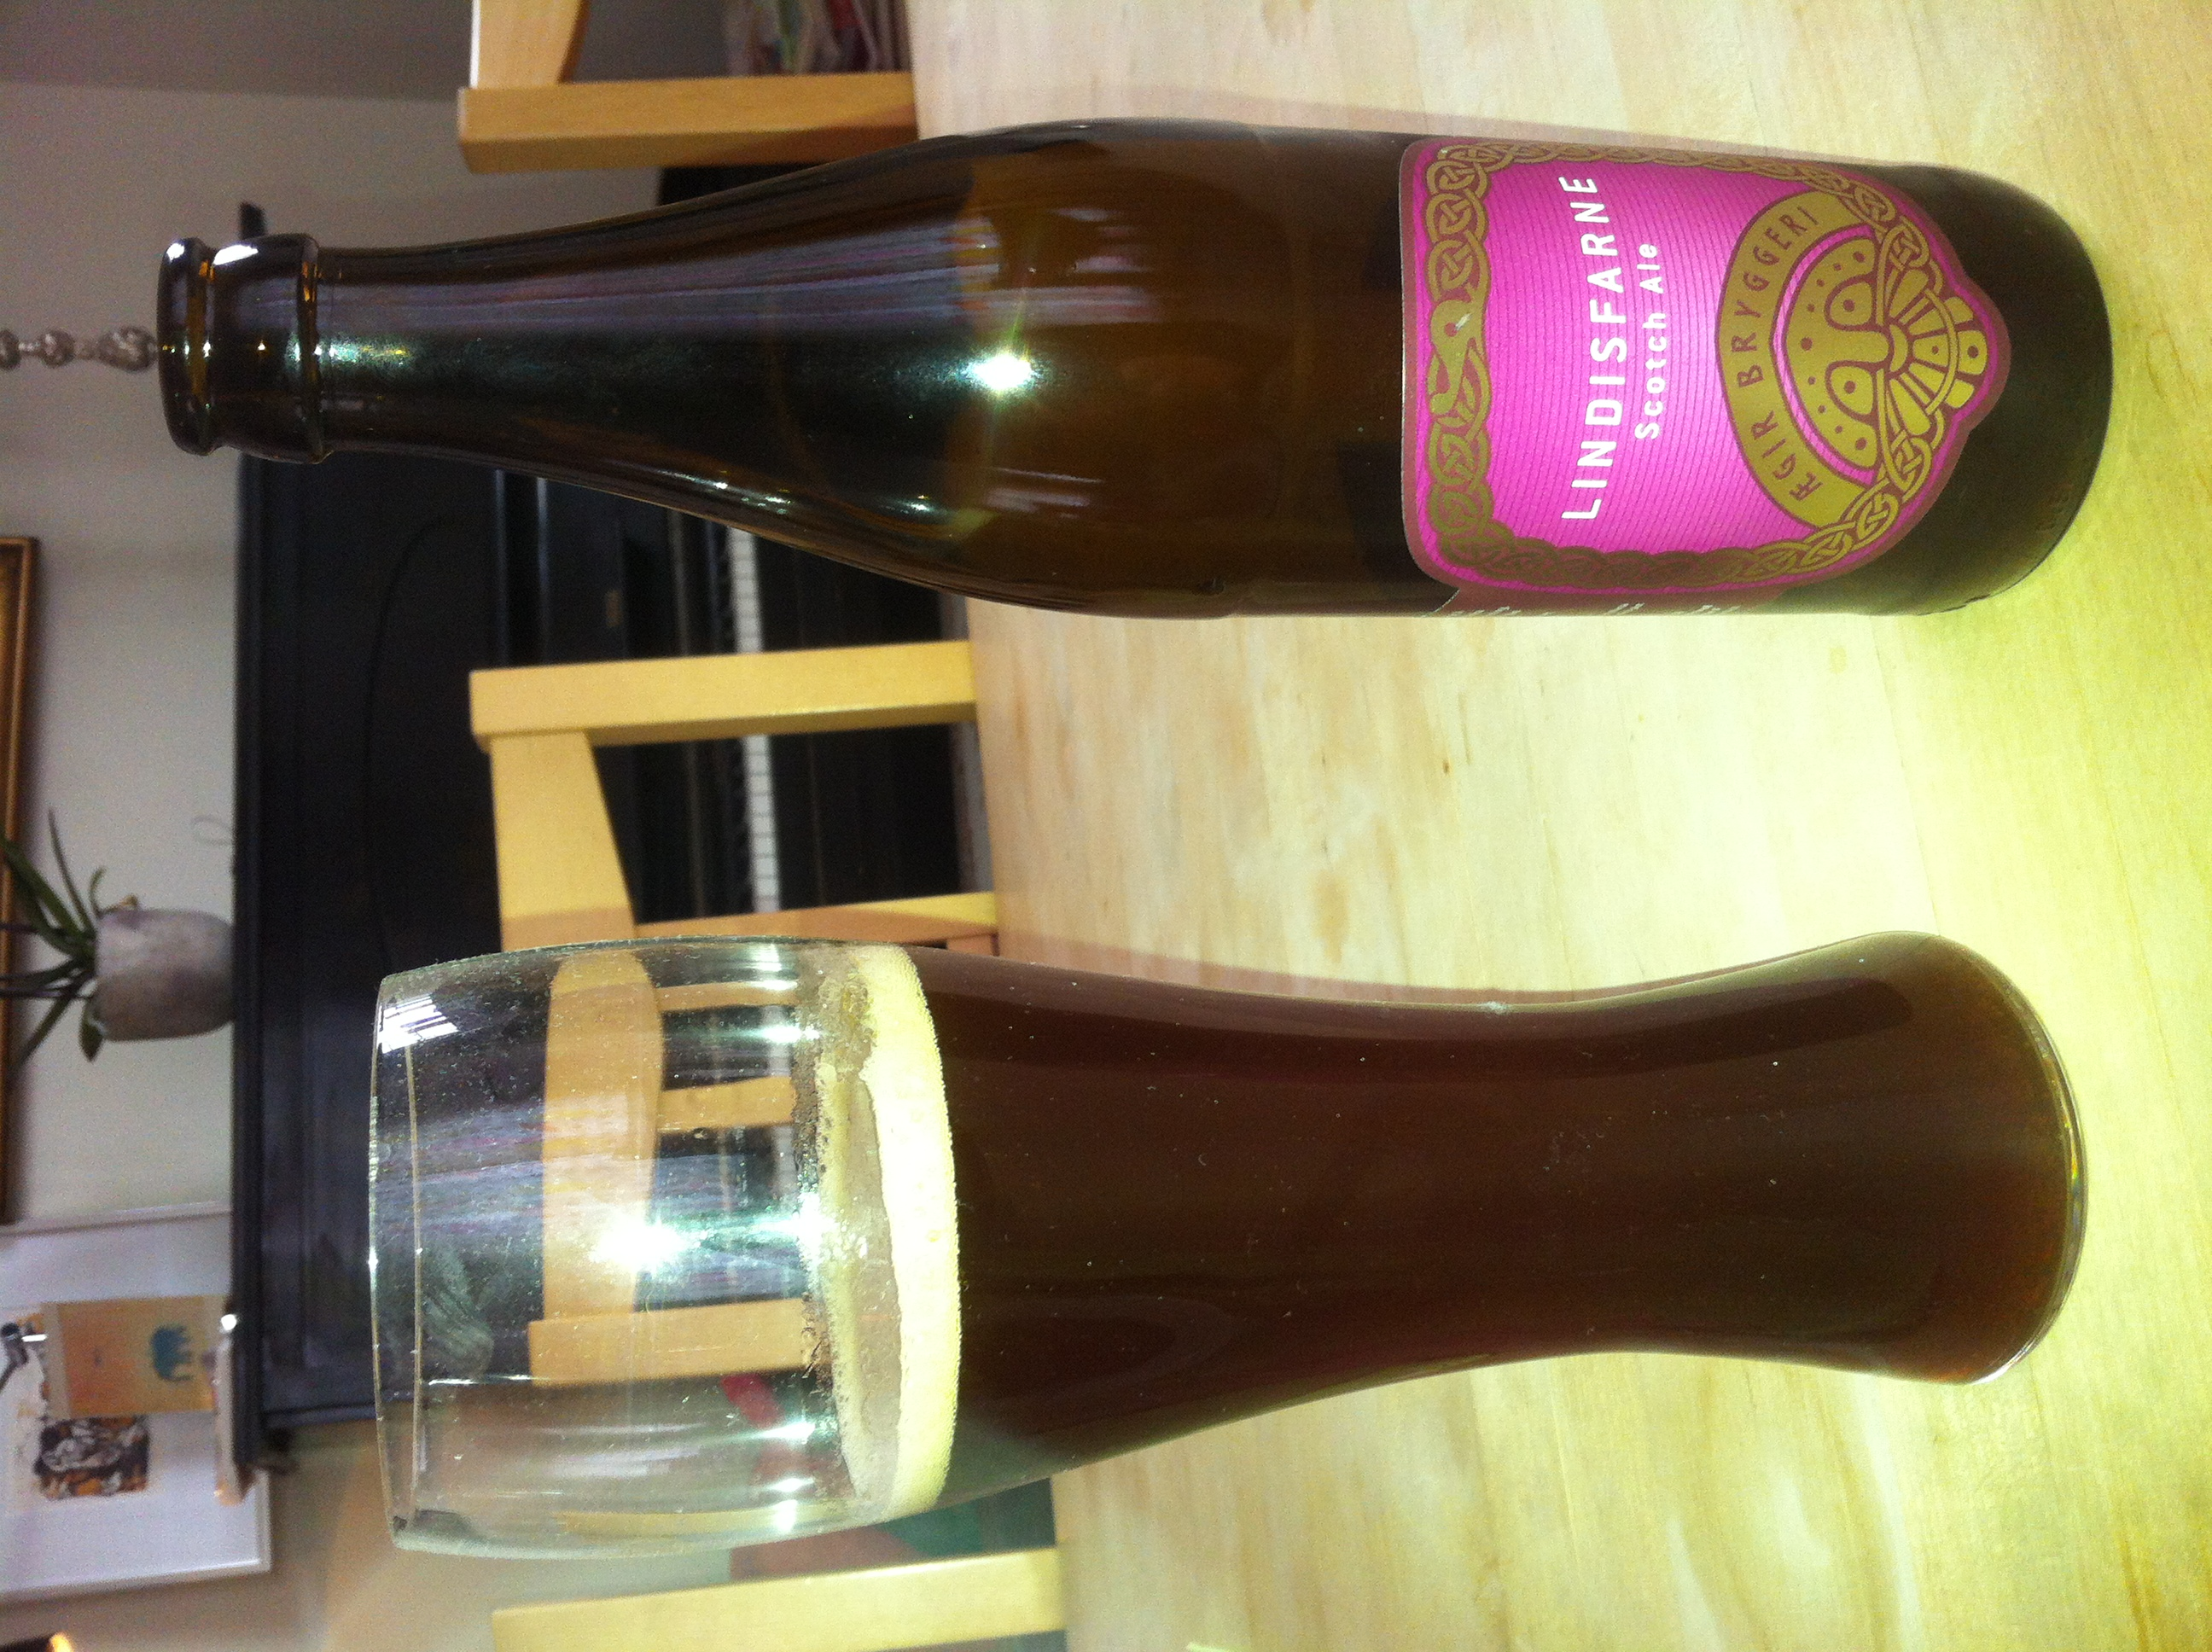
\includegraphics[scale=0.1, angle=270]{Bilder/Ol/lindisfarne}
\caption{Lindisfarne Scotch Ale fra Ægir Bryggeri}
\end{figure}

\newpage
\subsubsection{Robinsons Family Brewers: Iron Maiden Trooper}
\paragraph{Kommentar:}Litt som å kjøpe Beats by Dre. Det er en helt grei øl, men når du kjøper den i Norge så betaler for merkevaren. Mild og lett smak. 
\newline
-- -- Isak 04.06.2014


\begin{figure} [H]
\centering
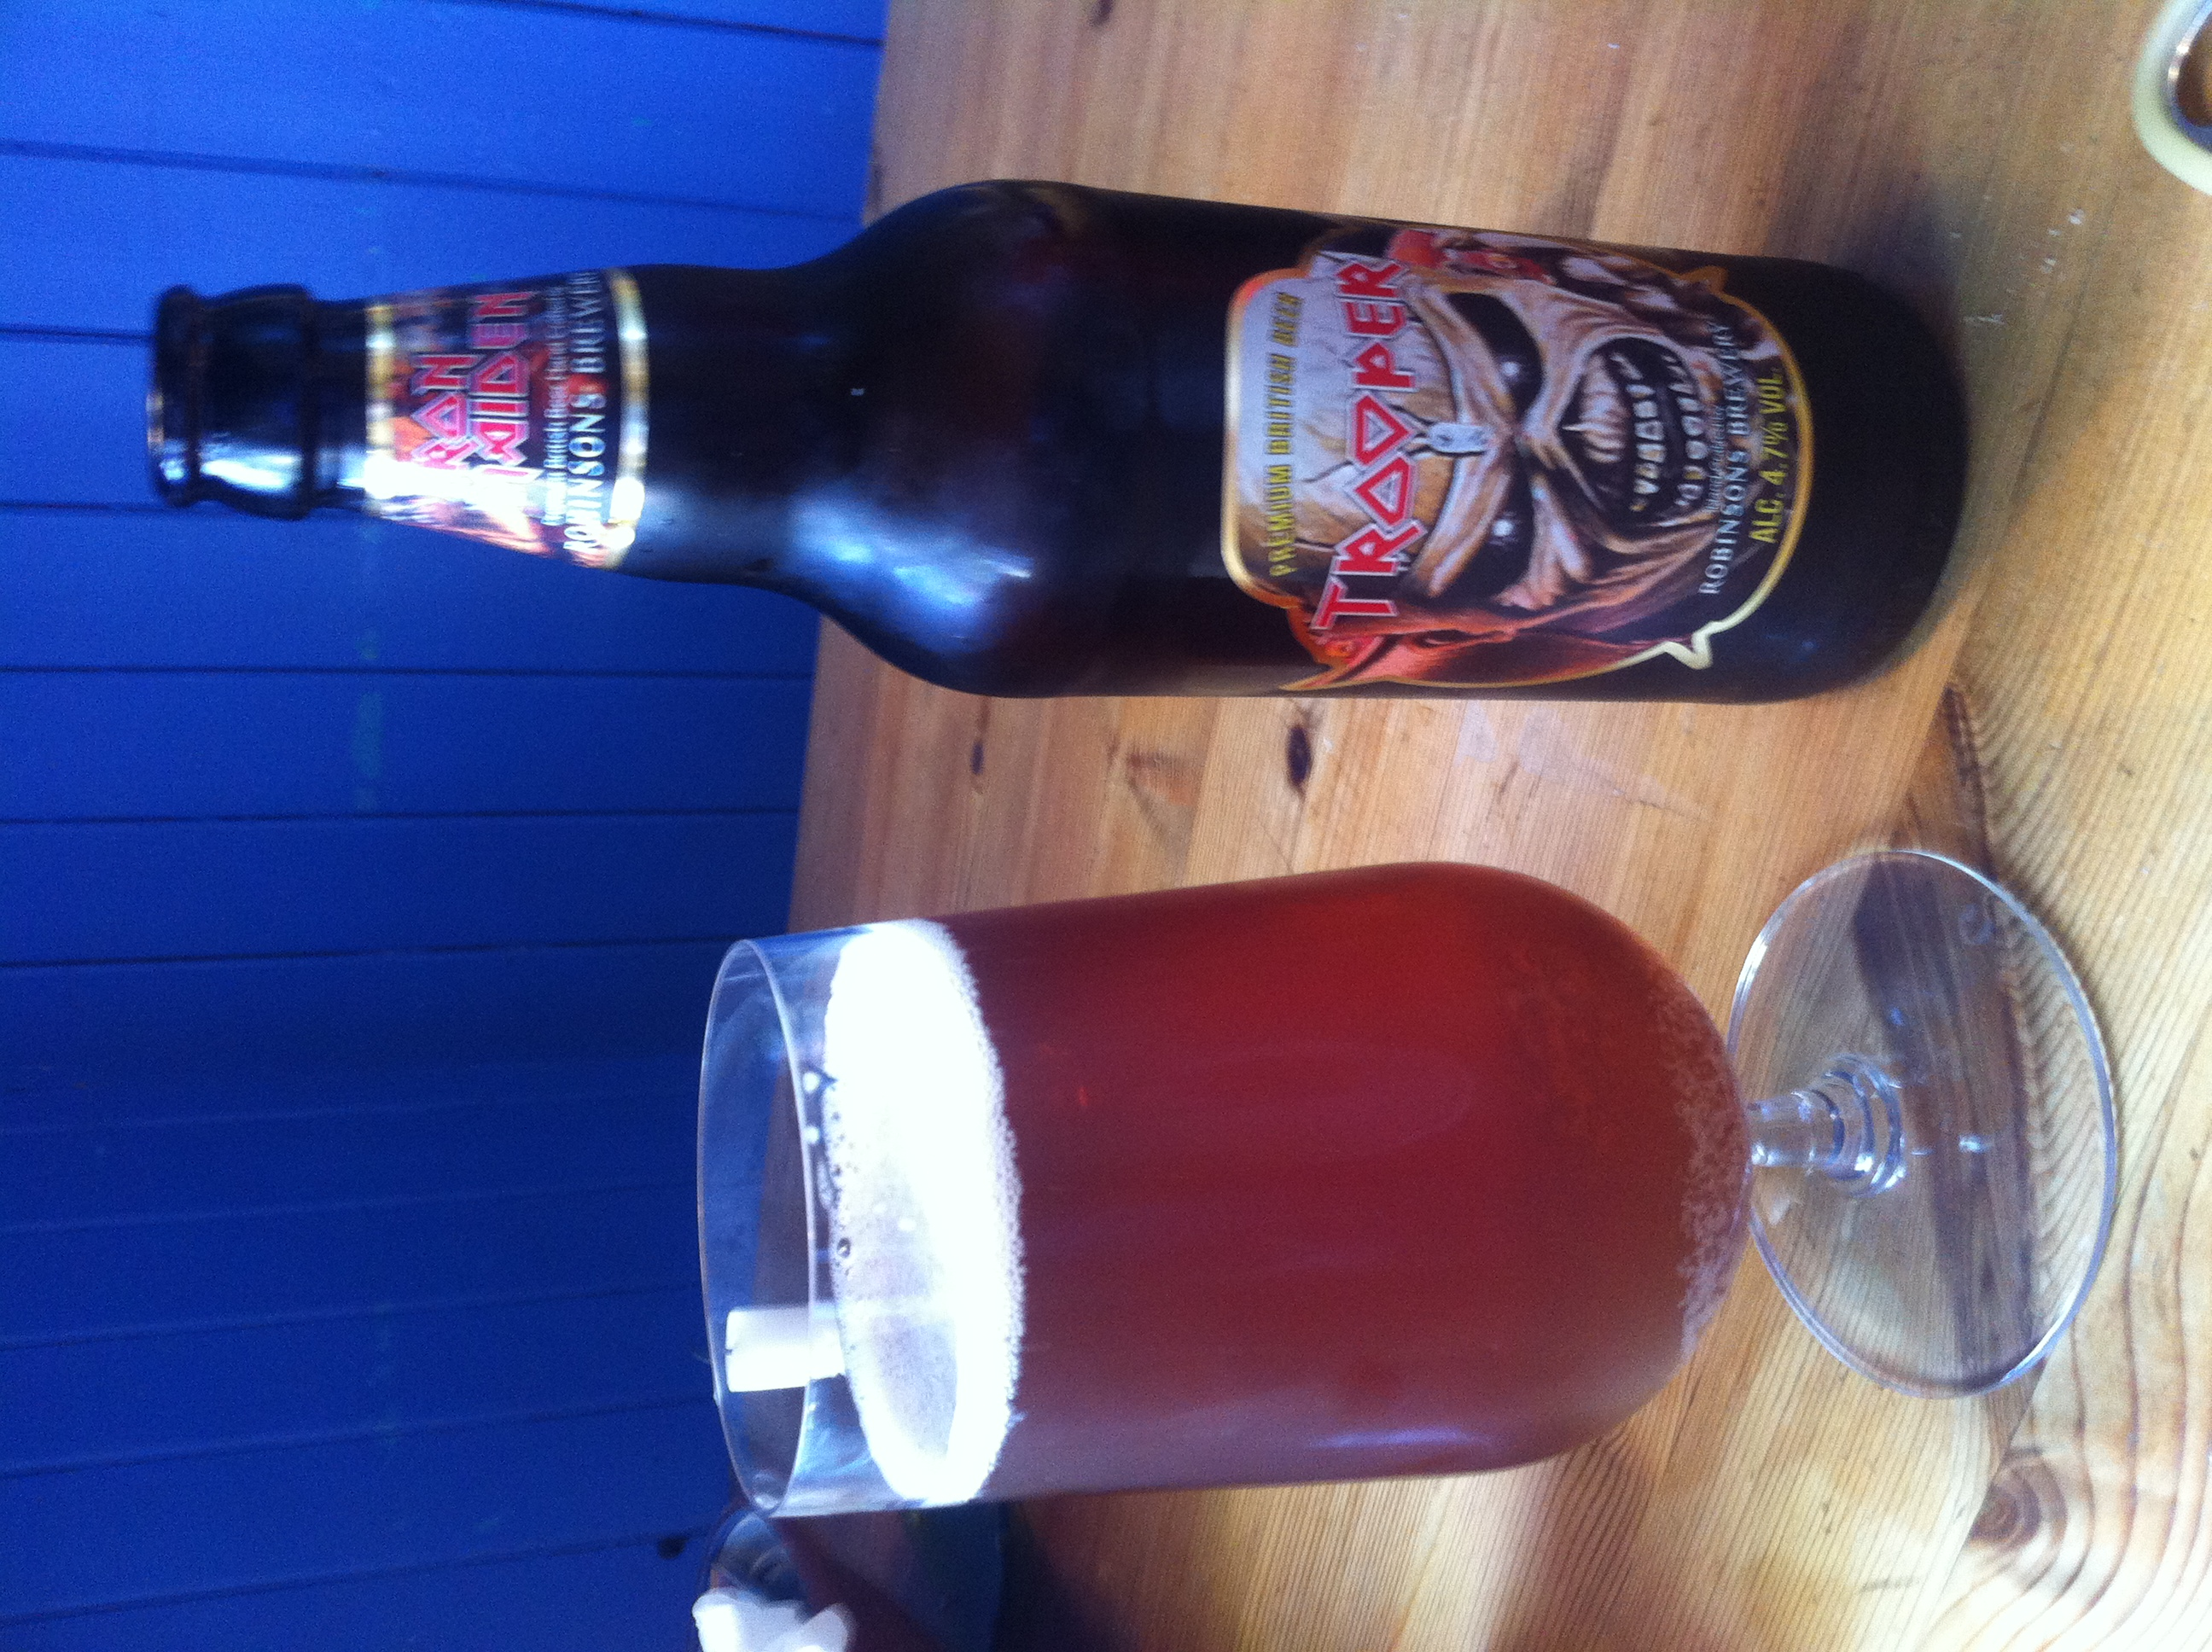
\includegraphics[scale=0.1, angle=270]{Bilder/Ol/thetrooper}
\caption{Iron Maiden Trooper fra Robinsons Family Brewers}
\end{figure}

\newpage
\subsubsection{NØGNE Ø: Blonde}
\paragraph{Kommentar:} En veldig god øl som er brygget i en Belgian Ale stil. Ikke 100 prosent hveteøl, som er et pluss i mine øyne. Forfriskende og god, men ikke spesielt bitter slik mange rene hveteøl kan være. Perfekt på en varm sommerdag. 
\newline
-- -- Isak 04.06.2014

\begin{figure} [H]
\centering
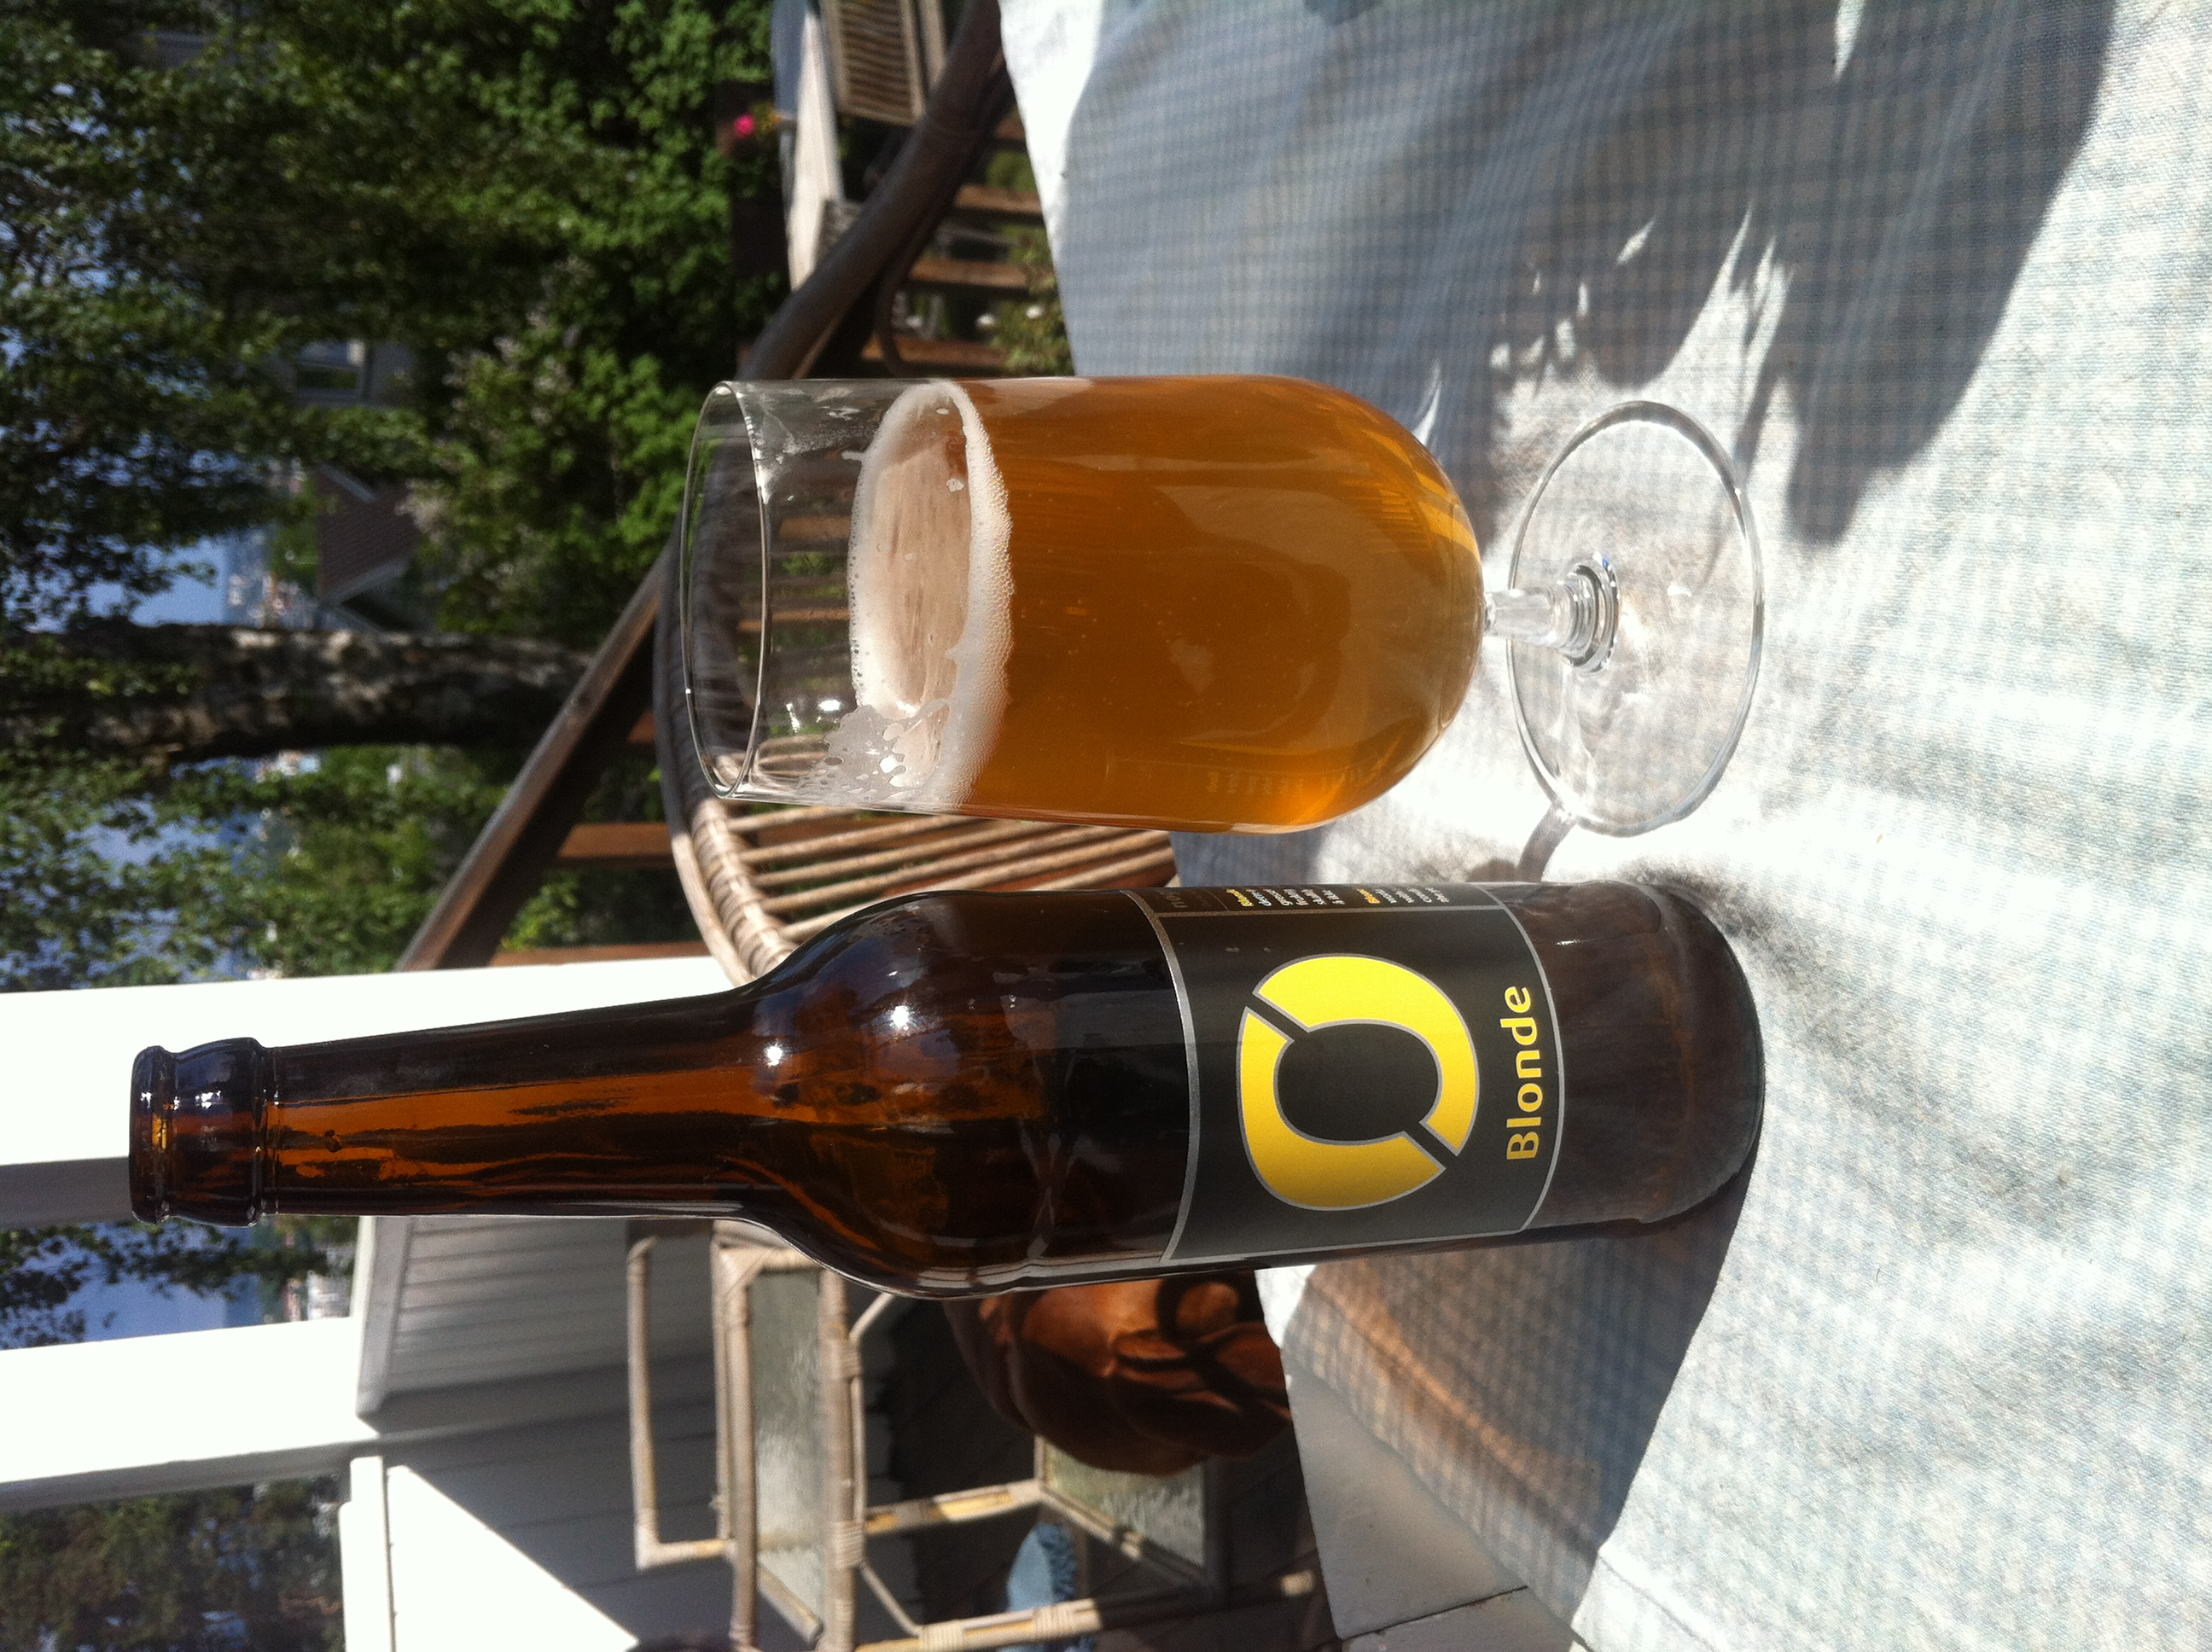
\includegraphics[scale=0.1, angle=270]{Bilder/Ol/nogneblonde}
\caption{Blonde fra NØGNE Ø}
\end{figure}

\newpage
\subsubsection{Boulevard Brewing Co. : The Sixth Glass}
\paragraph{Kommentar:}Var litt sent på kvelden da jeg drakk denne ølen, så ta dette med en klype salt. Dette er en quadrupel ale, jeg vet ikke hva det betyr. Den var søt og veldig fyldig. Trolig bra at den var søt så den kamuflerer den høye alkoholprosenten. I følge Internett så er denne ølen i verdensklasse. Syn at jeg ikke er spesielt fan av søt øl, men til å være søt var ølen bra og vært å prøve. Prisen var ganske stram, men igjen kjøper man import øl på bar som klokker inn på 10,5 \%, er kanskje en litt høy pris å forvente. 
\newline
-- -- Anders 6.08.2014

\begin{figure} [H]
\centering
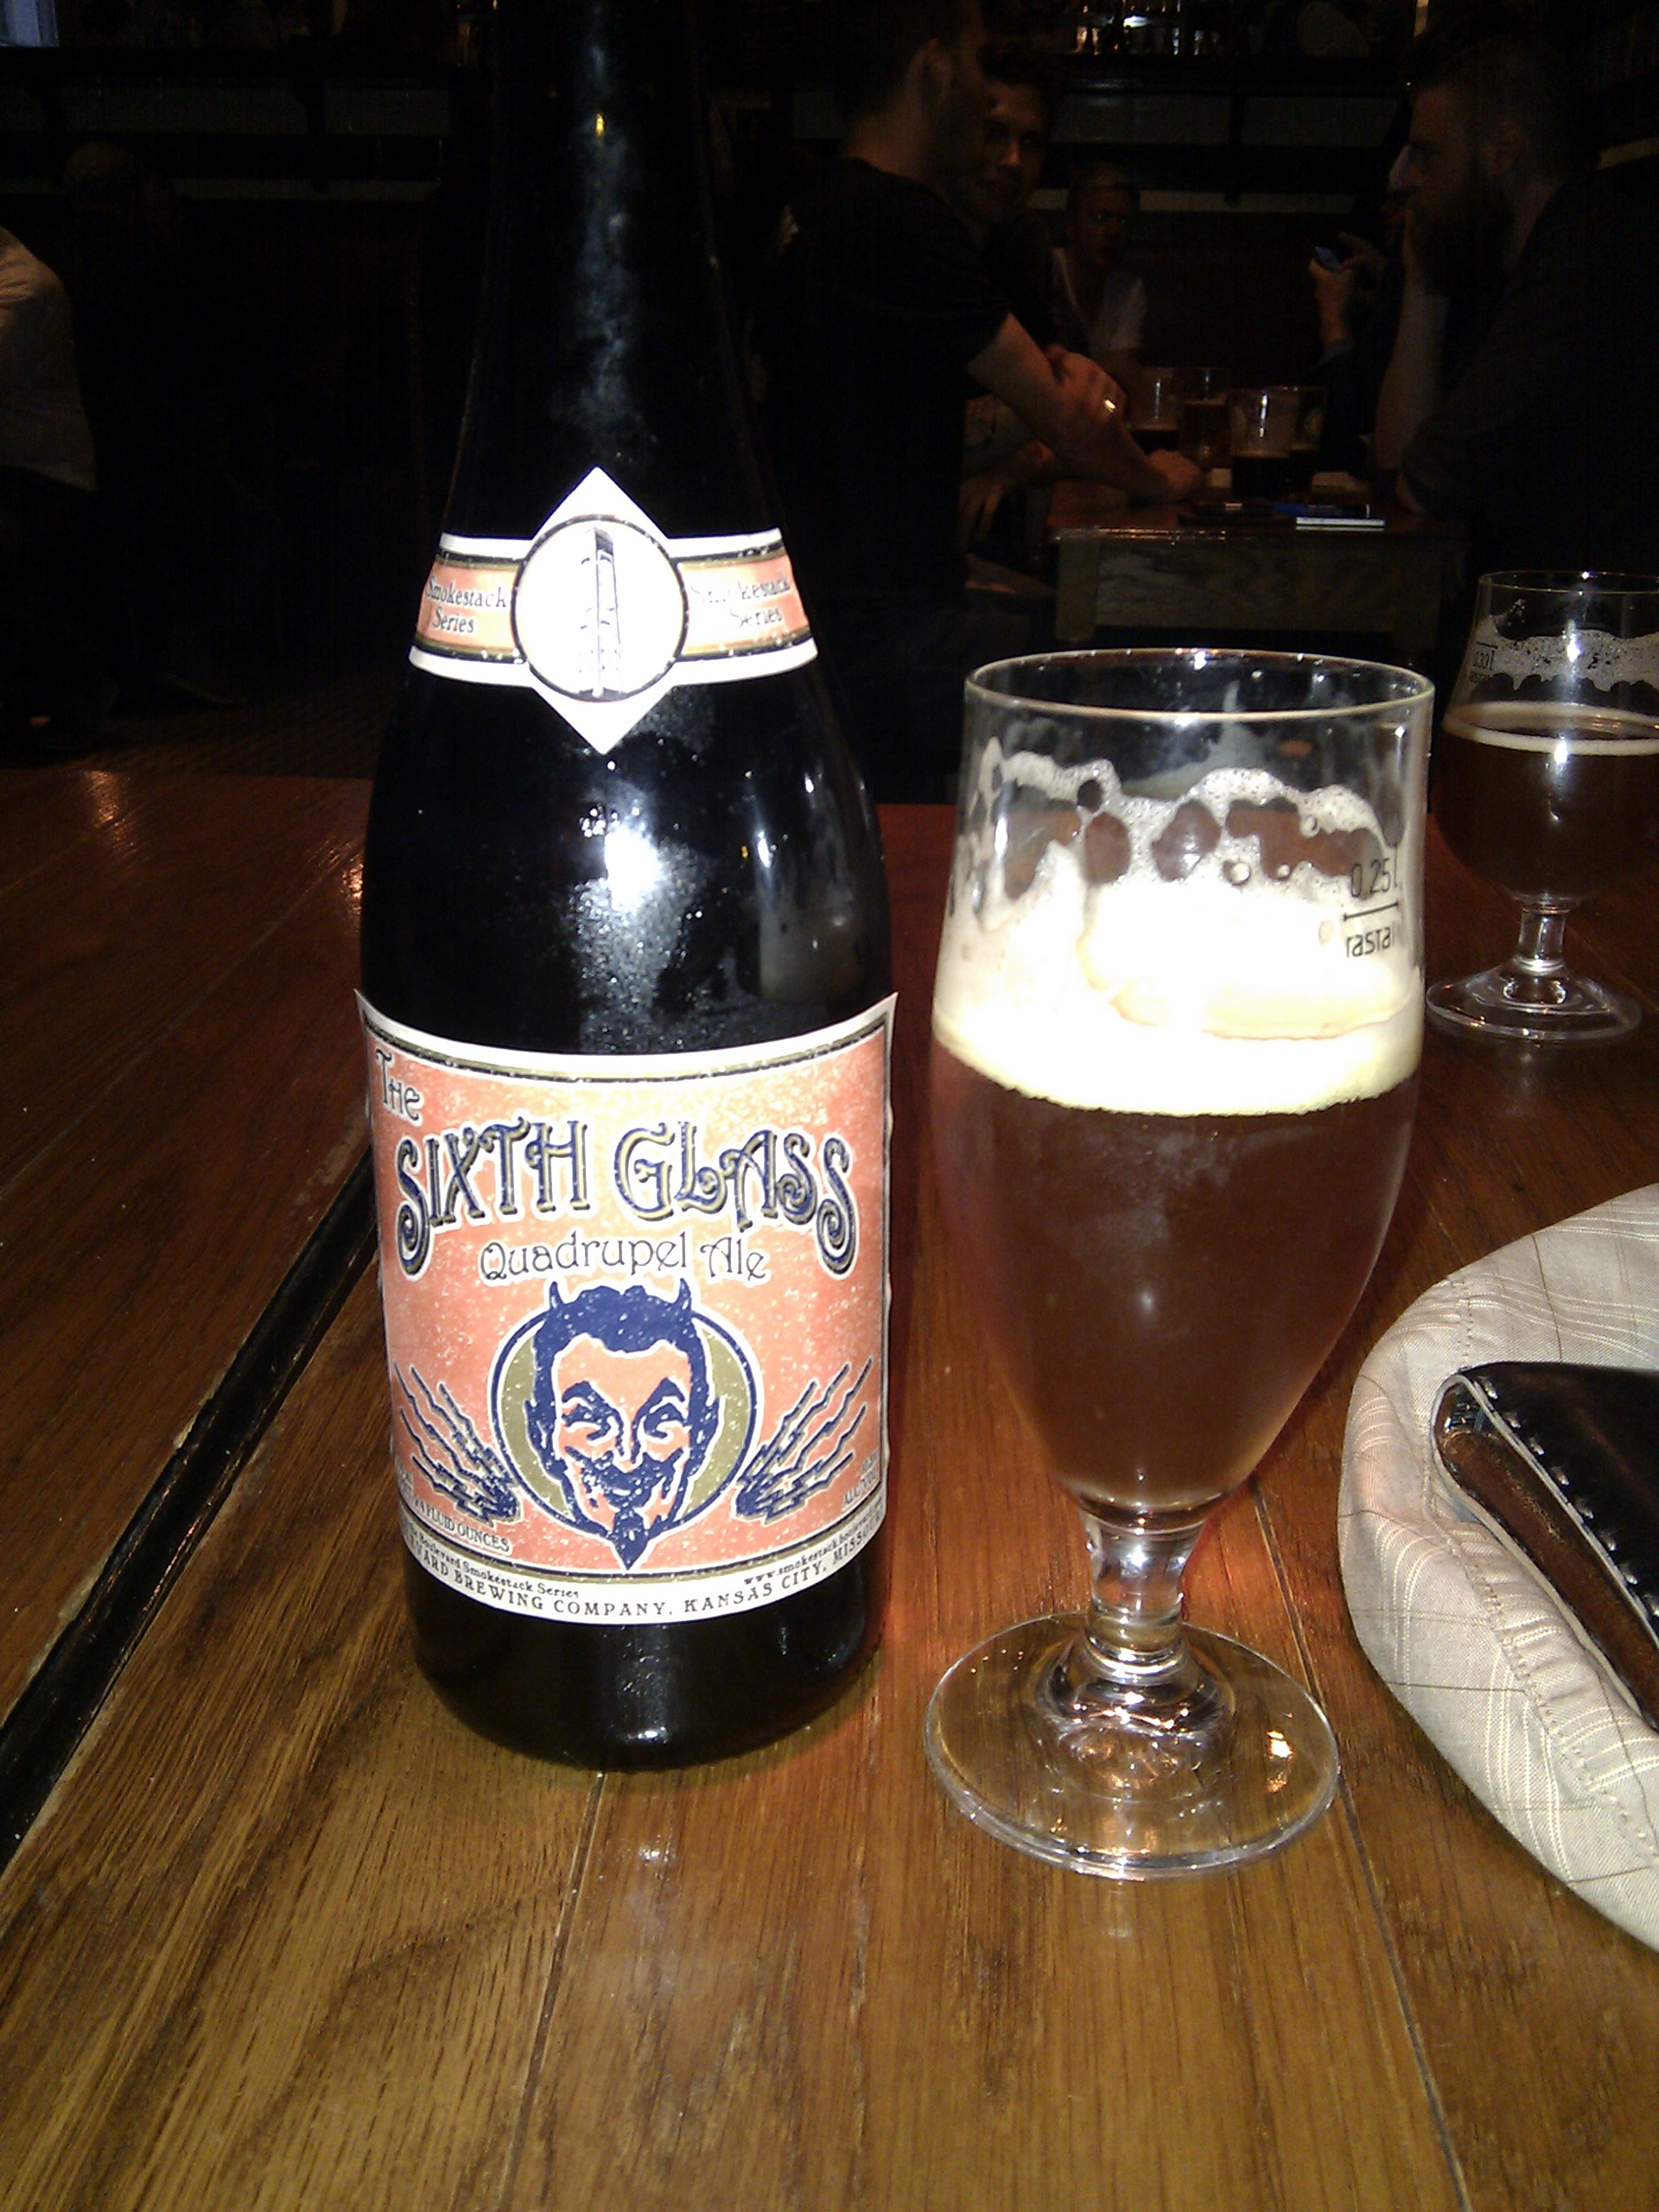
\includegraphics[scale=0.1, angle=0]{Bilder/Ol/Thesixth}
\caption{The Sixth Glass fra Boulevard Brewing Co.}
\end{figure}

\newpage
\subsection{Pils}

\subsubsection{Det Lille Bryggeriet: Birkebeinerpils}
\paragraph{Kommentar:}Nok en skuffende øl fra Det Lille Bryggeriet. Kjedelig og en litt ubehagelig smak i svelget. 
\newline
-- -- Isak 13.04.2014

\begin{figure} [H]
\centering
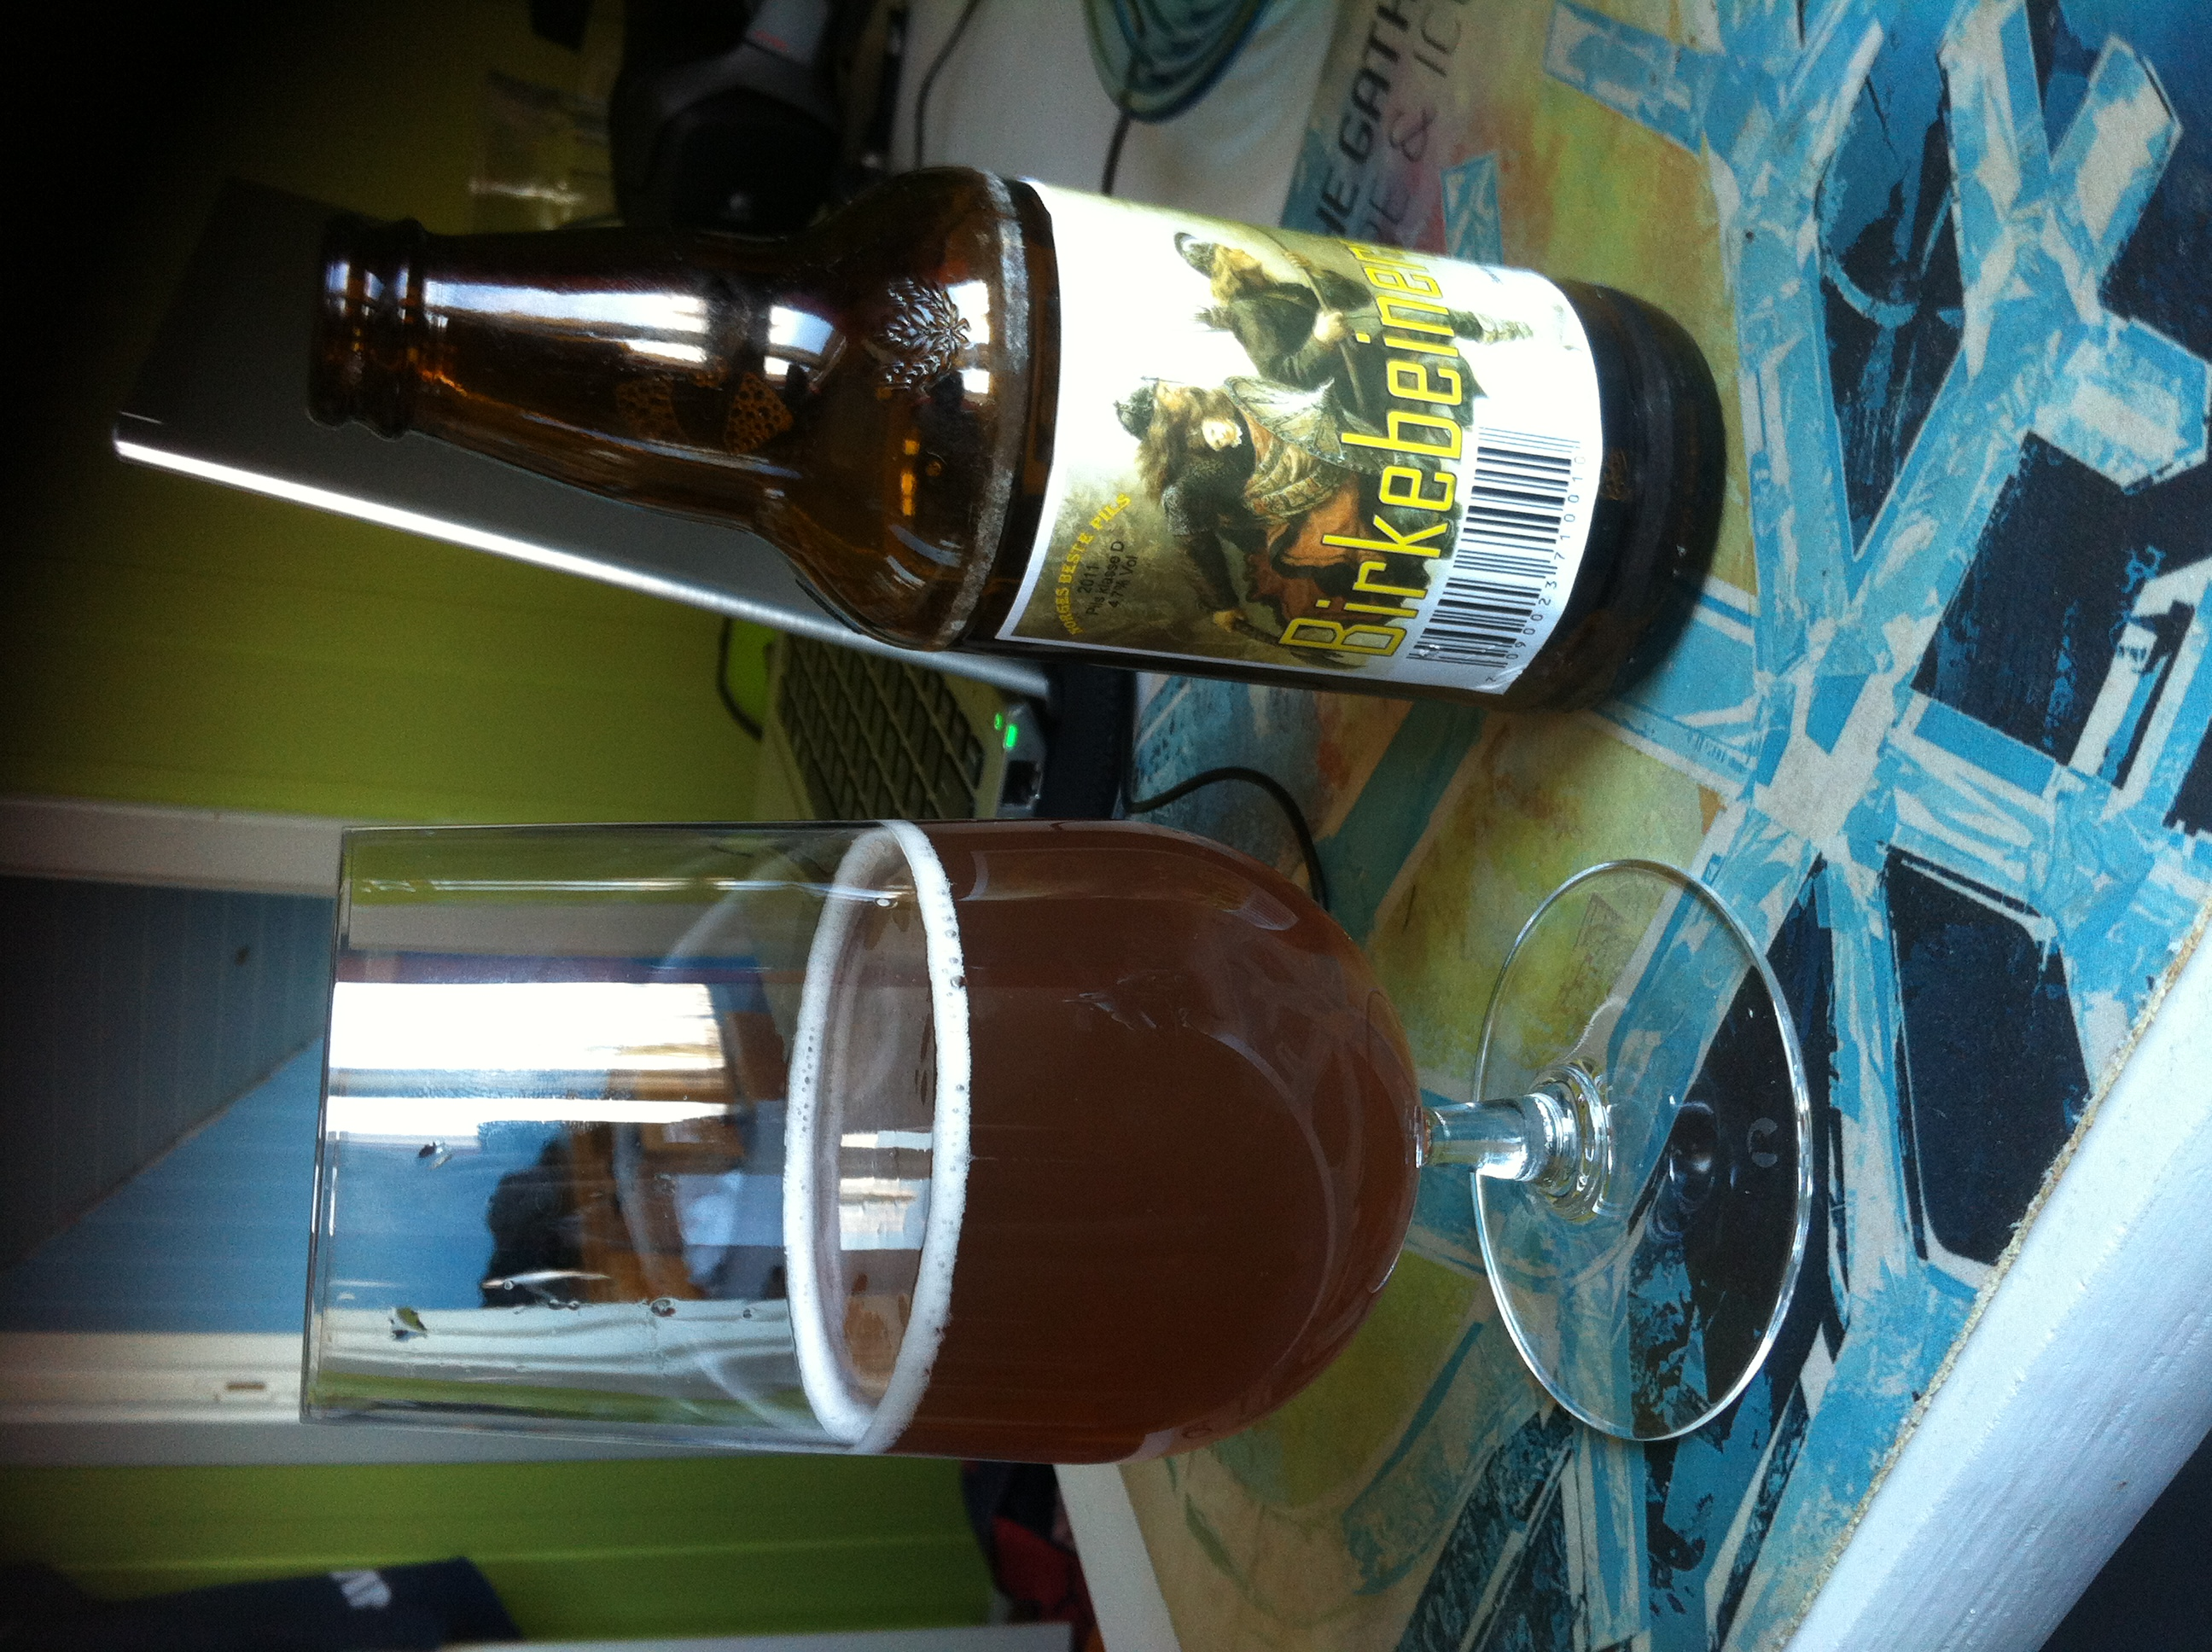
\includegraphics[scale=0.1, angle=270]{Bilder/Ol/birkebeiner.jpg}
\caption{Birkebeinerpils fra "Det Lille Bryggeriet"}
\end{figure}

\newpage
\subsubsection{E.C. Dahls Bryggeri: Dahls Pils}
\paragraph{Kommentar:}En ok industripils til prisen man betaler for den. Den har et preg av banan og fargen er som morgen-piss. Nytes best full, kan like gjerne drikkes rett fra flasken som fra glass. Da sparer man litt oppvask. Selv om ølen har et kipt industripreg, er den vist nok gunstig for bartevekst. Bivirkning ved ølen er utydelig tale og trang til å skyte inn med ordet "sjø" stadig vekk.
\newline
-- -- Anders 13.04.2014

\begin{figure} [H]
\centering
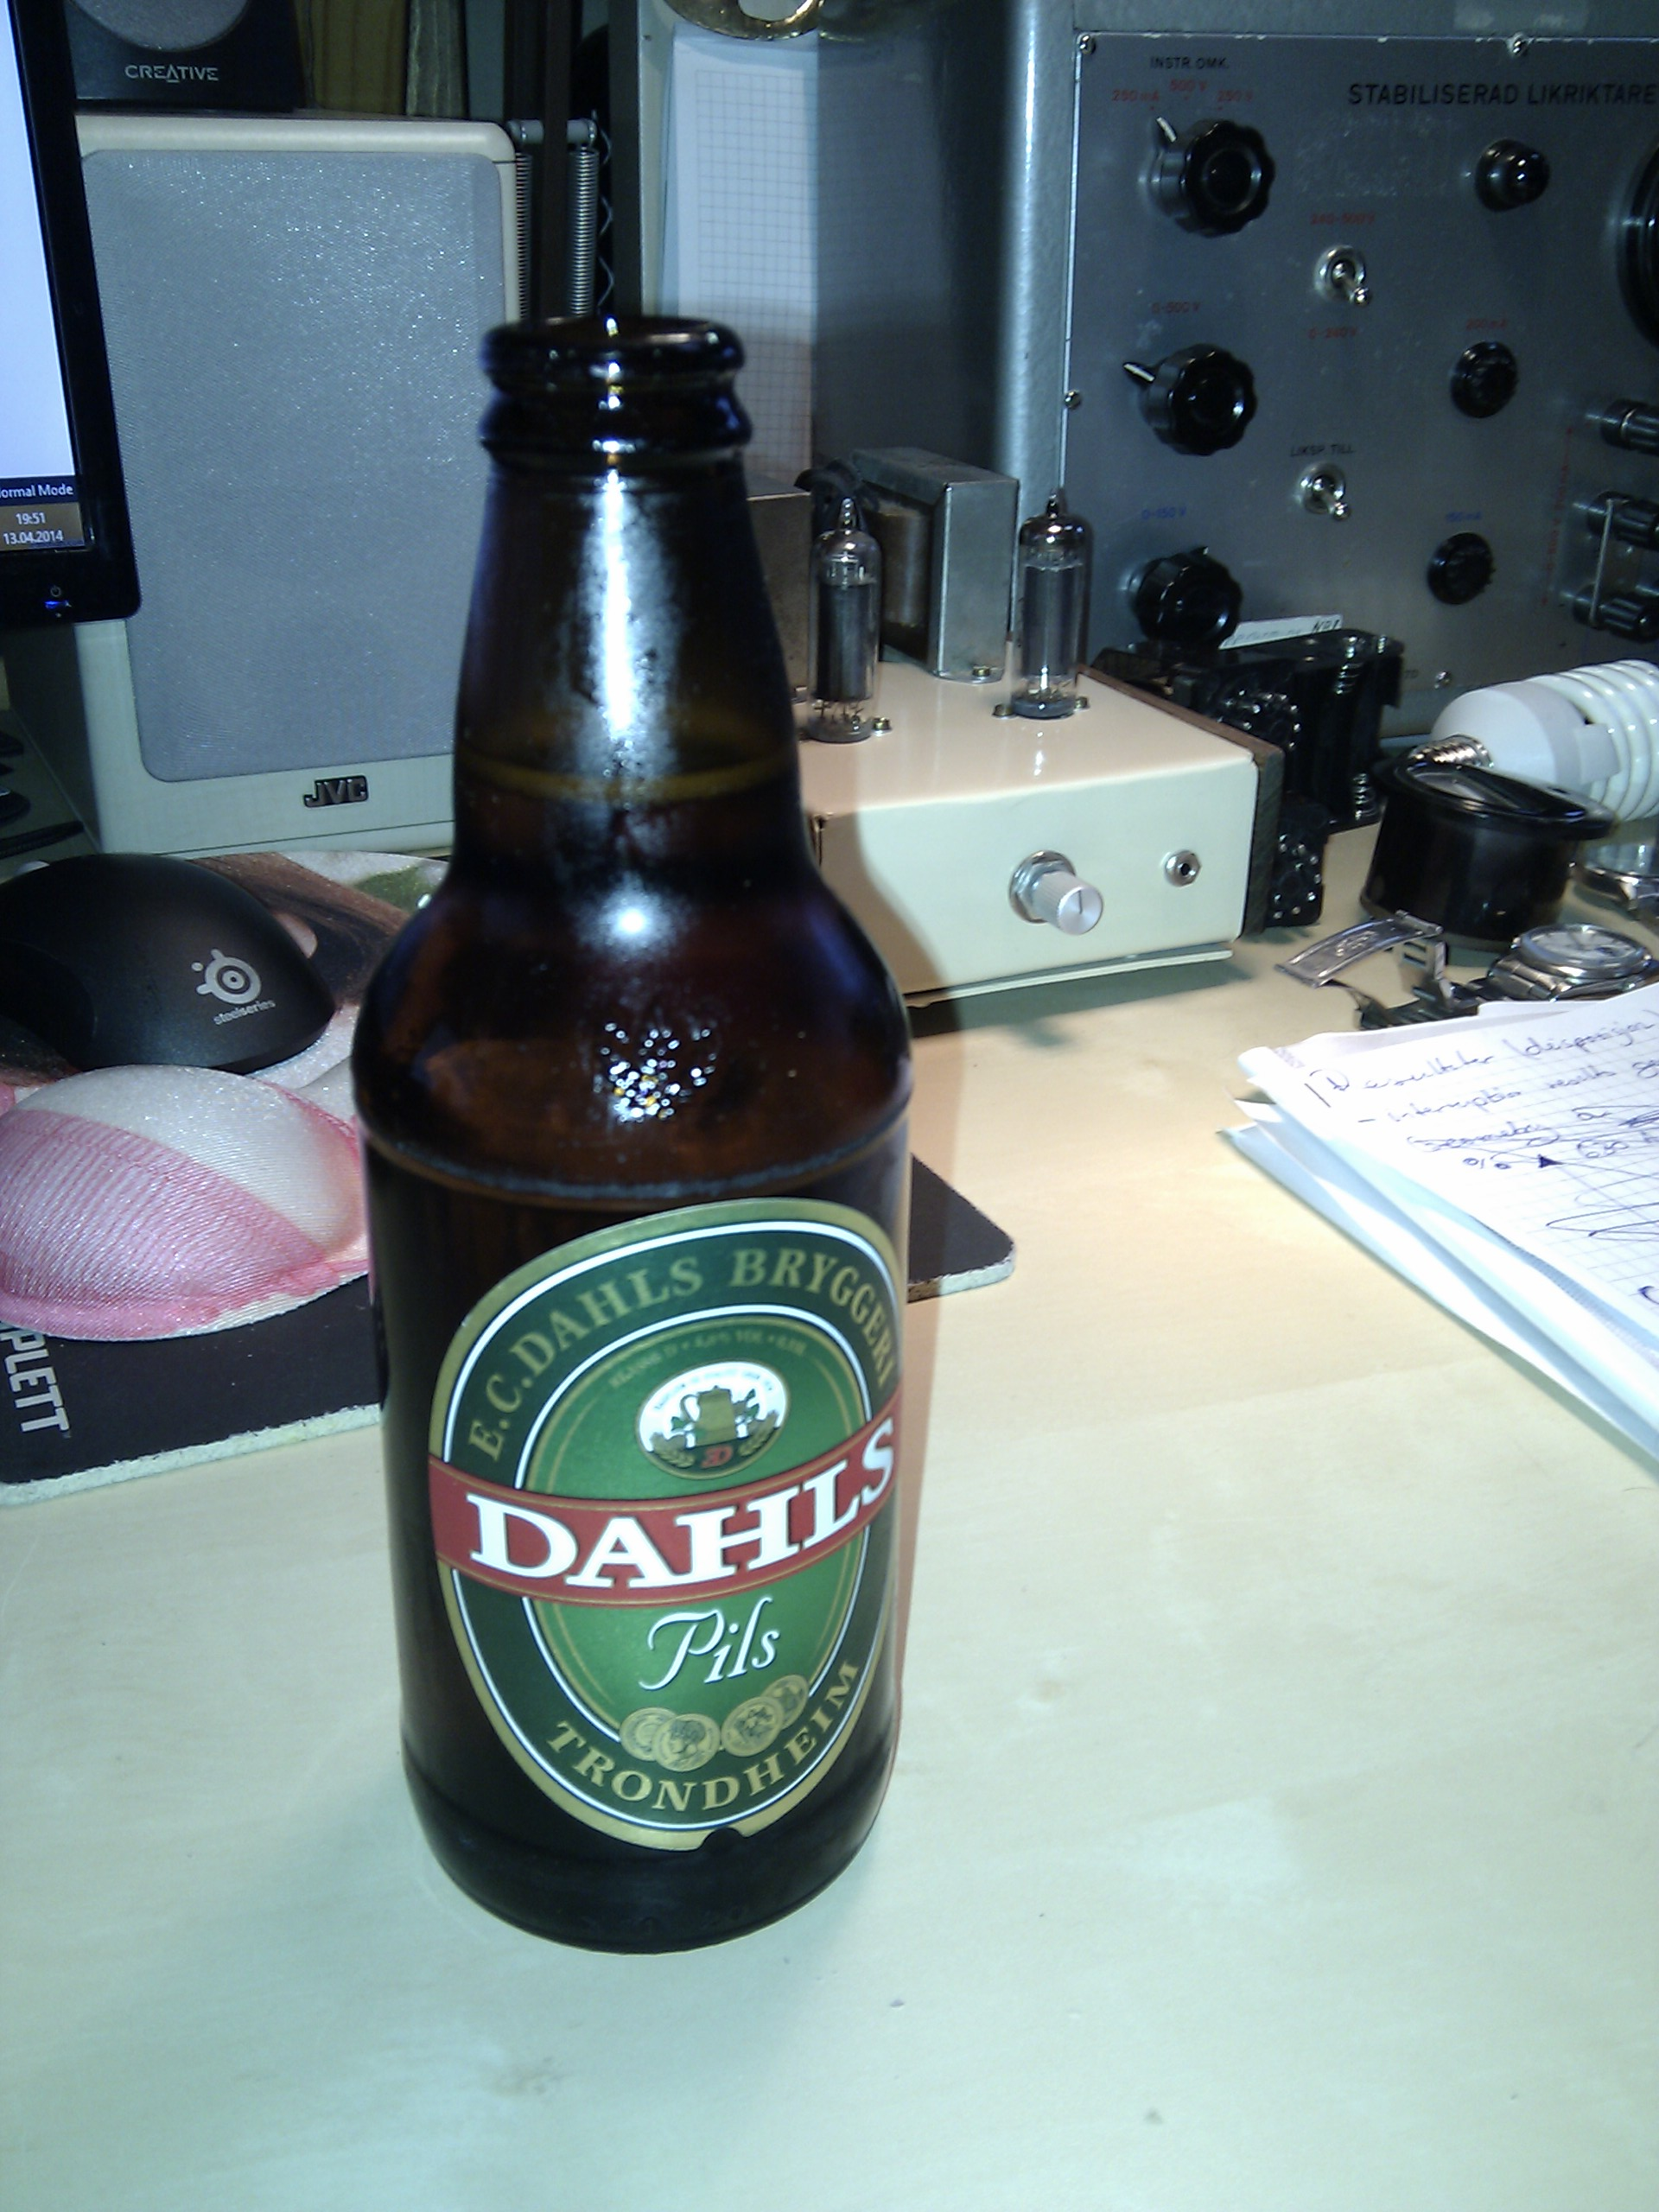
\includegraphics[scale=0.1, angle=0]{Bilder/Ol/dahls.jpg}
\caption{Dahls Pils fra "E.C. Dahls Bryggeri"}
\end{figure}

\newpage
\subsubsection{Grans Bryggeri: Lade Gaards Brygghus Pilsner}
\paragraph{Kommentar:}Ok, det er tre ting som er bra, eller faktisk fantastisk med denne pilsen. Den har skrukork, blir servert i halvliter flasker, men det beste av alt er: på innsiden av skrukorken er det et bilde av en neve som viser stein, saks, eller papir! Dette er fantastisk og nyskapende! Nå kan de av oss som drikker øl sammen med andre, faktisk spille stein, saks, papir uten å ta et valg selv. Nydelig! Det til side, smaksmessig er ølen helt ok, det er jo en typisk industripils, men er betydelig bedre enn mye annet ræl man får kjøpt på matbutikken. Uansett blir ølen for dyr når den koster nesten 80 kr literen. Finnes definitift bedre pils til den prisen. Jeg ville anbefale folk å prøve denne engang, men mest fordi: "skrukork og halvliter". Hvorfor selges ikke flere butikkpils med skrukork og i halvliter flasker?
\newline
-- -- Anders 25.04.2014

\begin{figure} [H]
\centering
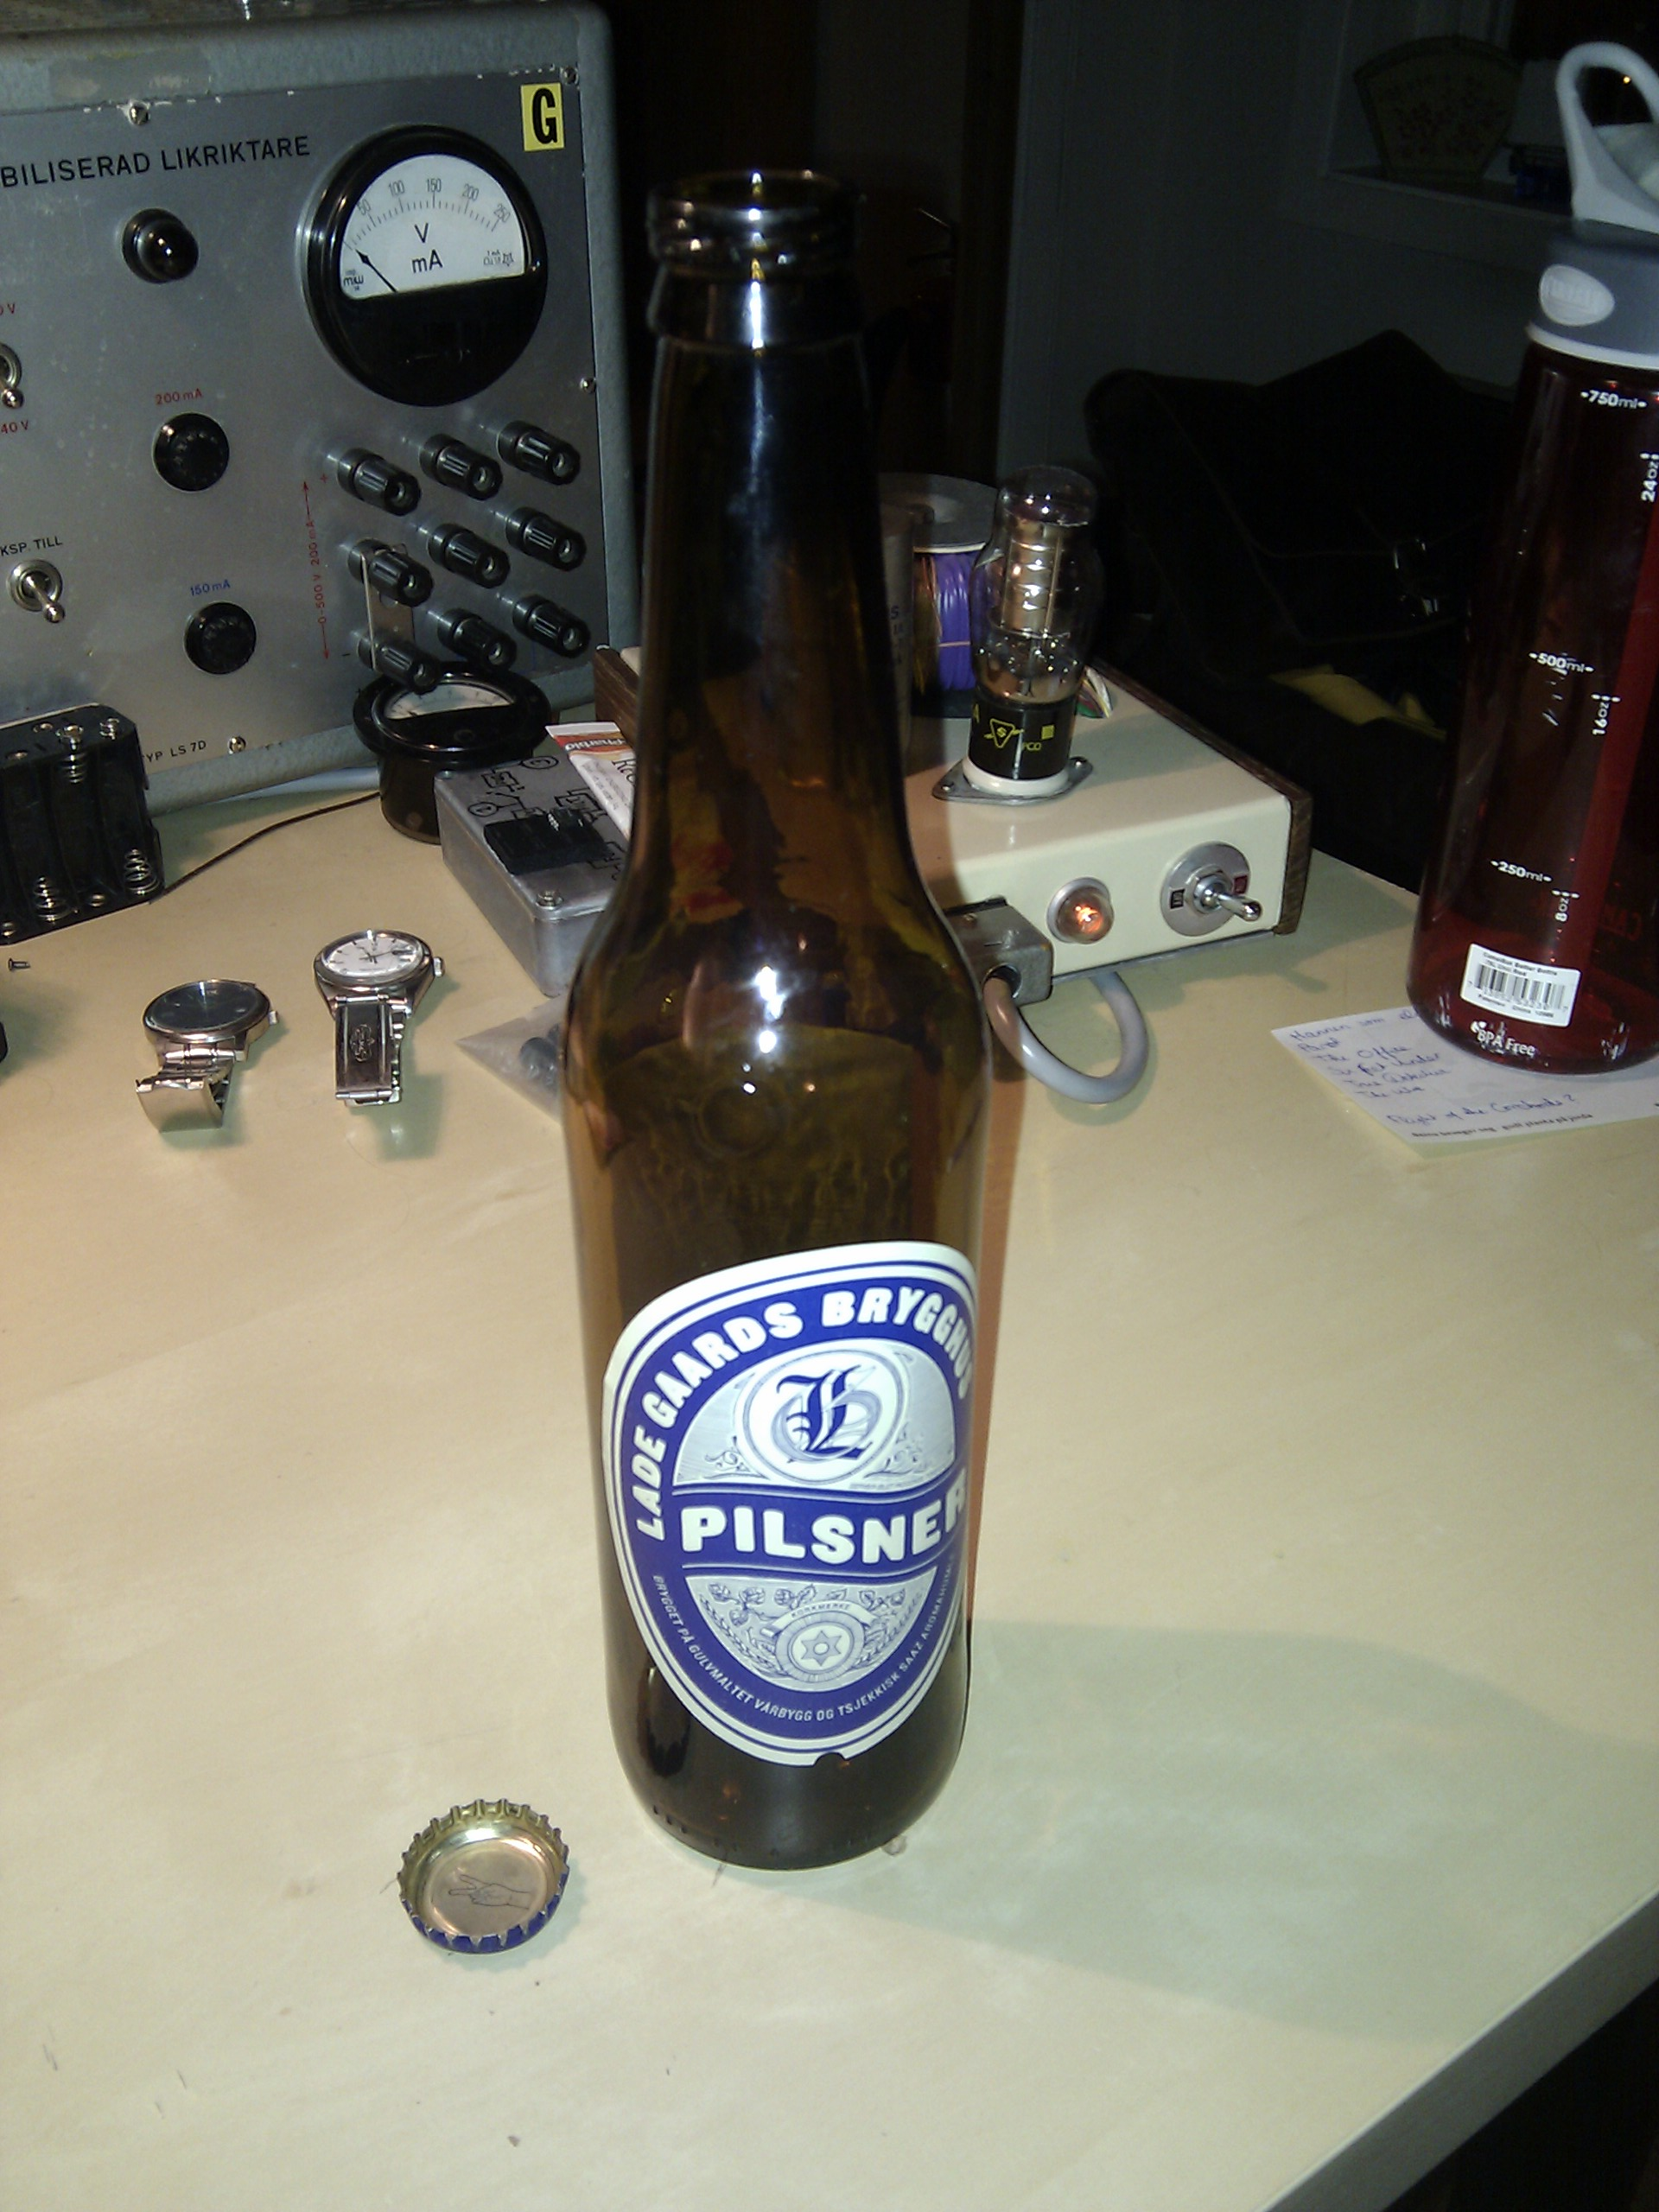
\includegraphics[scale=0.1, angle=0]{Bilder/Ol/ladeGaardPils.jpg}
\caption{Lade Gaards Brygghus Pilsner fra "Grans Bryggeri"}
\end{figure}

\newpage
\subsubsection{Nordlands Bryggeri: Nordlands Pils}
\paragraph{Kommentar:}Det er rart at man prøver å selge en sommerpils fra Nord-Norge. Det er svært lite sommerlig ved Nord-Norge. Som Dahlsen nytes denne også best full, kan like gjerne drikkes rett fra flasken som fra glass. På flasken står det at det er mye hygge i en nordlending. Det stemmer nok, men nordlendingen drikker nok Mack. Det kan være nordlendingen benytter seg av en knust flaske Nordlands Pils når de trenger stikkvåpen fordi hans fetteren nettopp dumpet hans søster til fordel for en russisk import-brud. Pilsen har et litt søtlig krydder preg over seg, og er veldig lys i fargen. Den er relativt smakløs nesten som vann, finnes sikkert noen som liker det å.
\newline
-- -- Anders 14.04.2014

\begin{figure} [H]
\centering
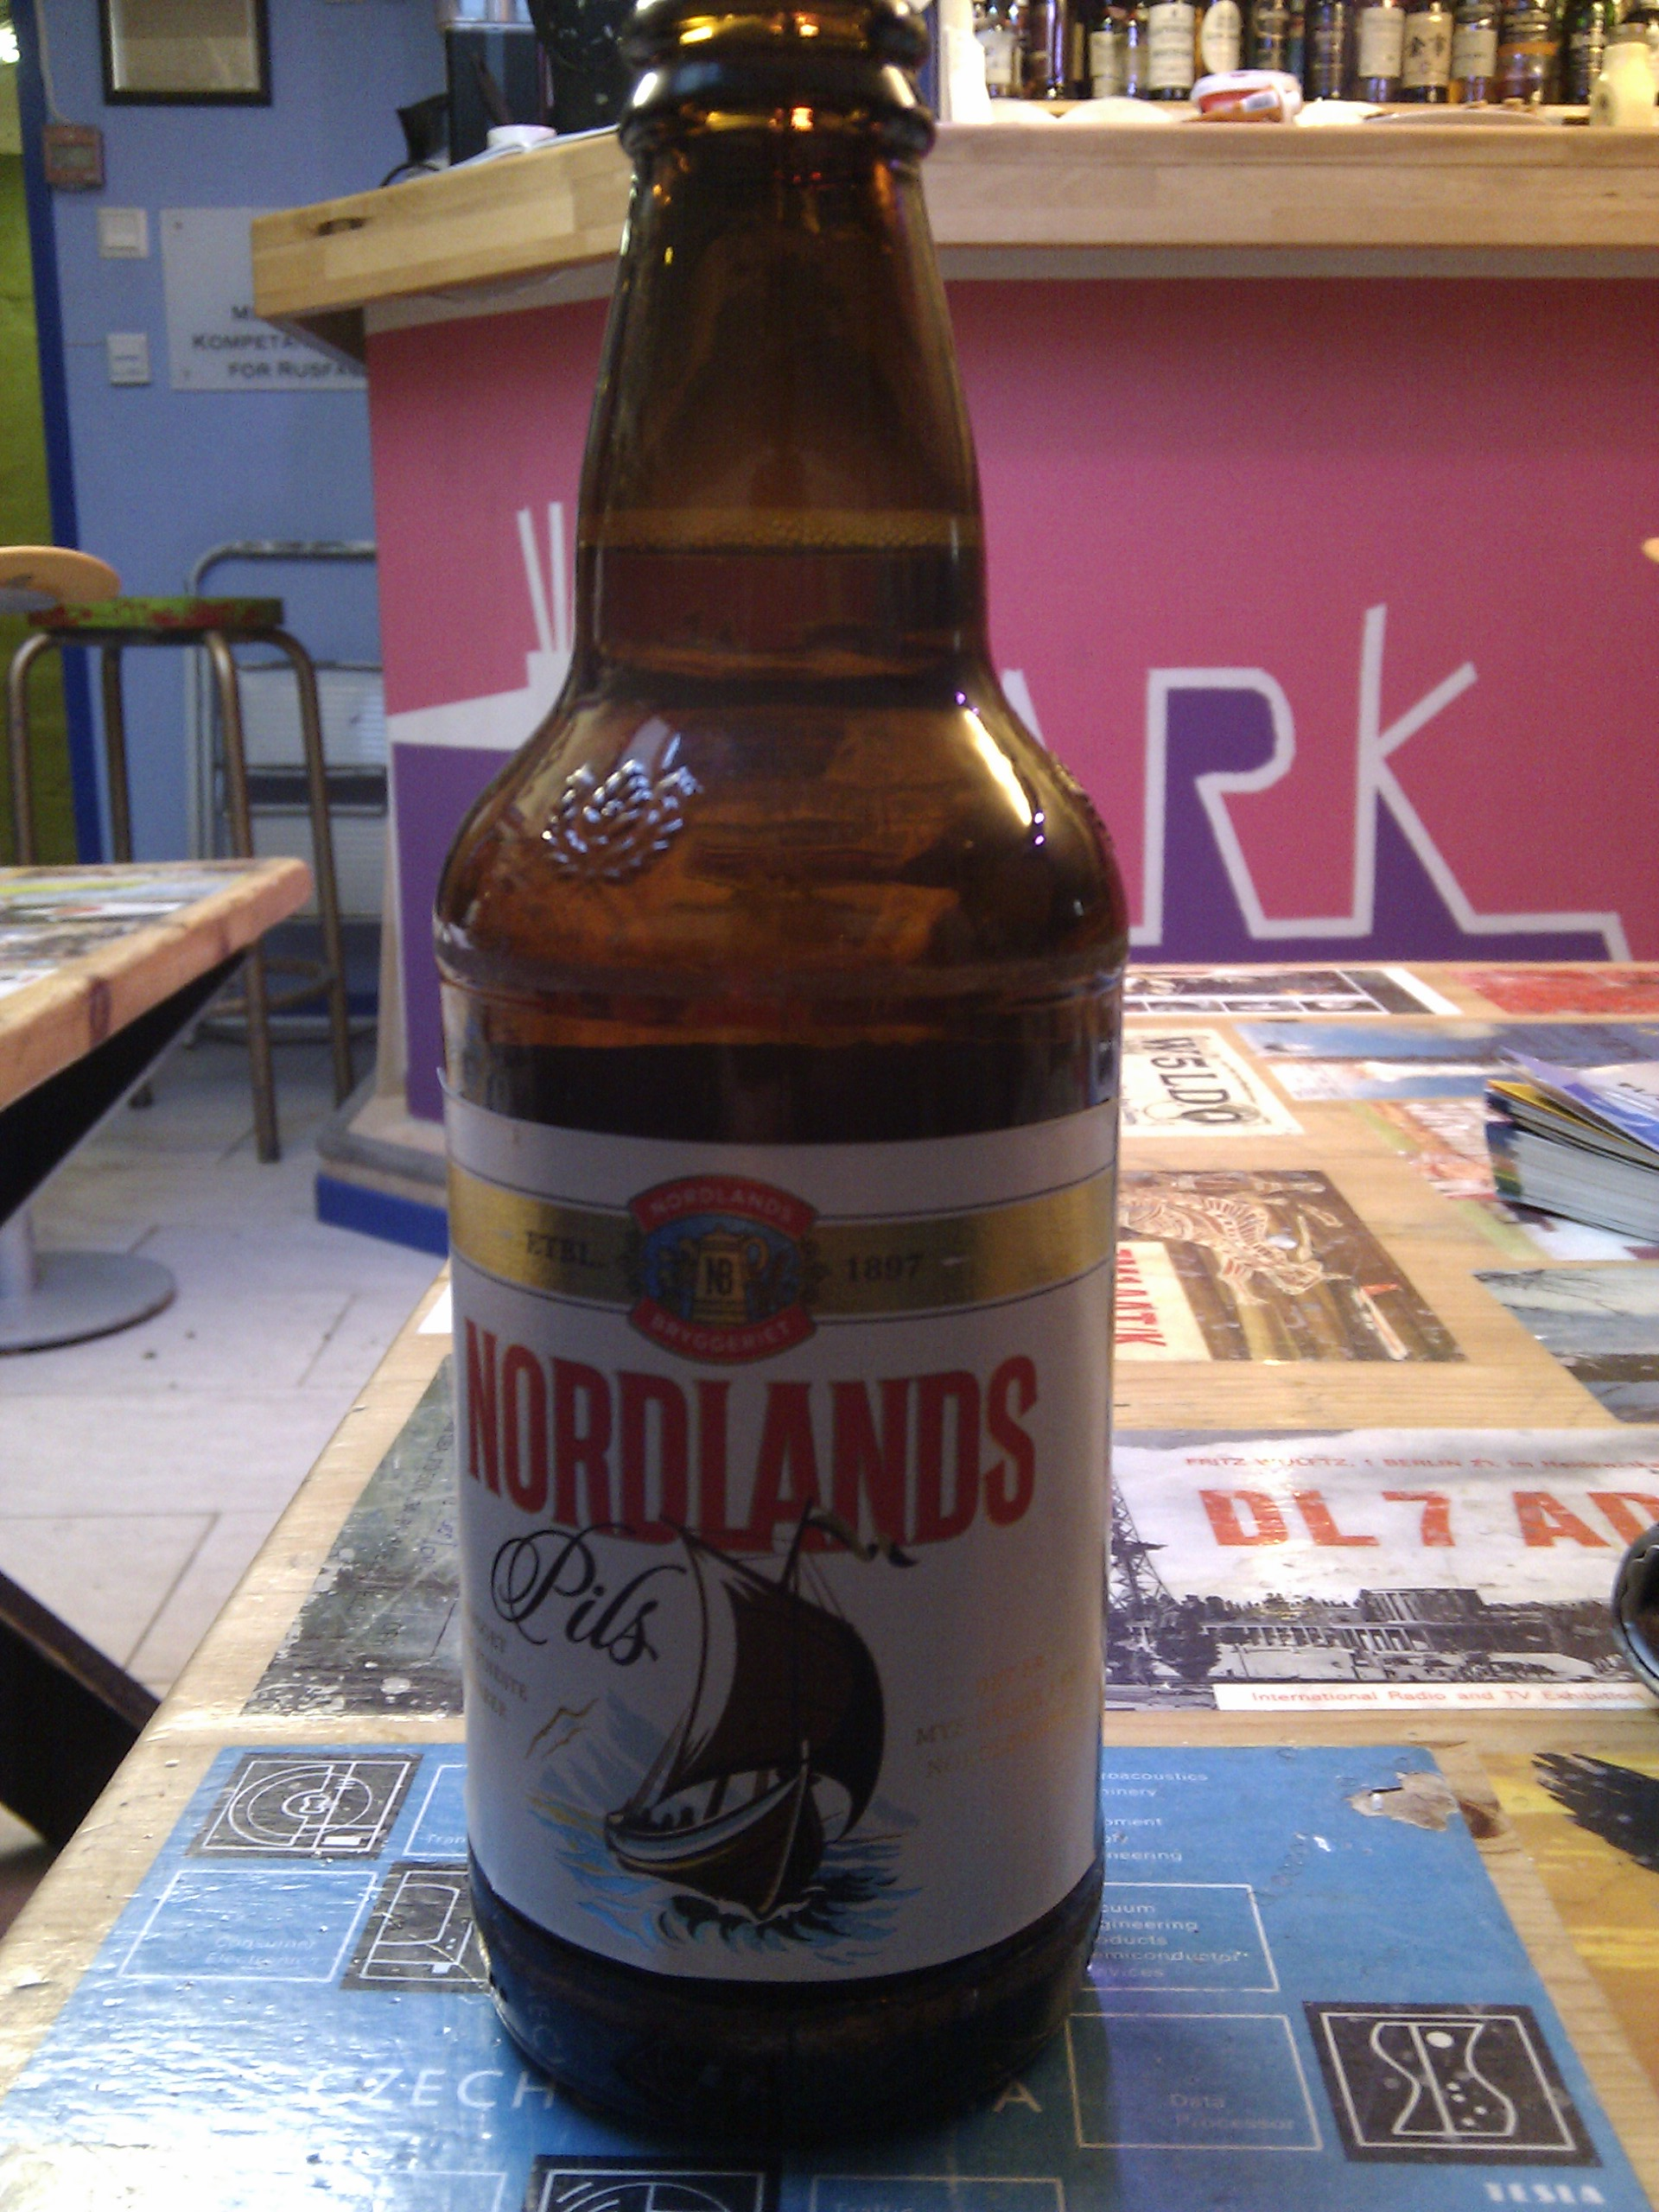
\includegraphics[scale=0.1, angle=0]{Bilder/Ol/NordlandsPils.jpg}
\caption{Nordlands Pils fra "Nordlands Bryggeri"}
\end{figure}

\newpage
\subsection{IPA}
\subsubsection{Austmann Bryggeri: Humledugg}
\paragraph{Kommentar:} Ikke blant de rammeste IPA'ene, men har som en IPA skal ha et tydelig bittert preg. Om jeg først skal kjøpe IPA, tror jeg at jeg ville gått for andre varianter enn denne, rett å slett fordi den er i det litt mildeste laget. Om man derimot har lyst på en bitter øl (men ikke IPA bitter) er dette et godt valg. Den er riktig nok dyr i forhold til mengden du får, 0,33 l for over 50 lappen på polet er ikke spesielt rimelig. Hadde jeg fått en halv liter til den prisen hadde det vært lettere å forsvare prisen i forhold til kvaliteten. Ølen er forøvrig noe lysere enn den fremstår på bilde.
\newline
-- -- Anders 16.04.2014

\begin{figure} [H]
\centering
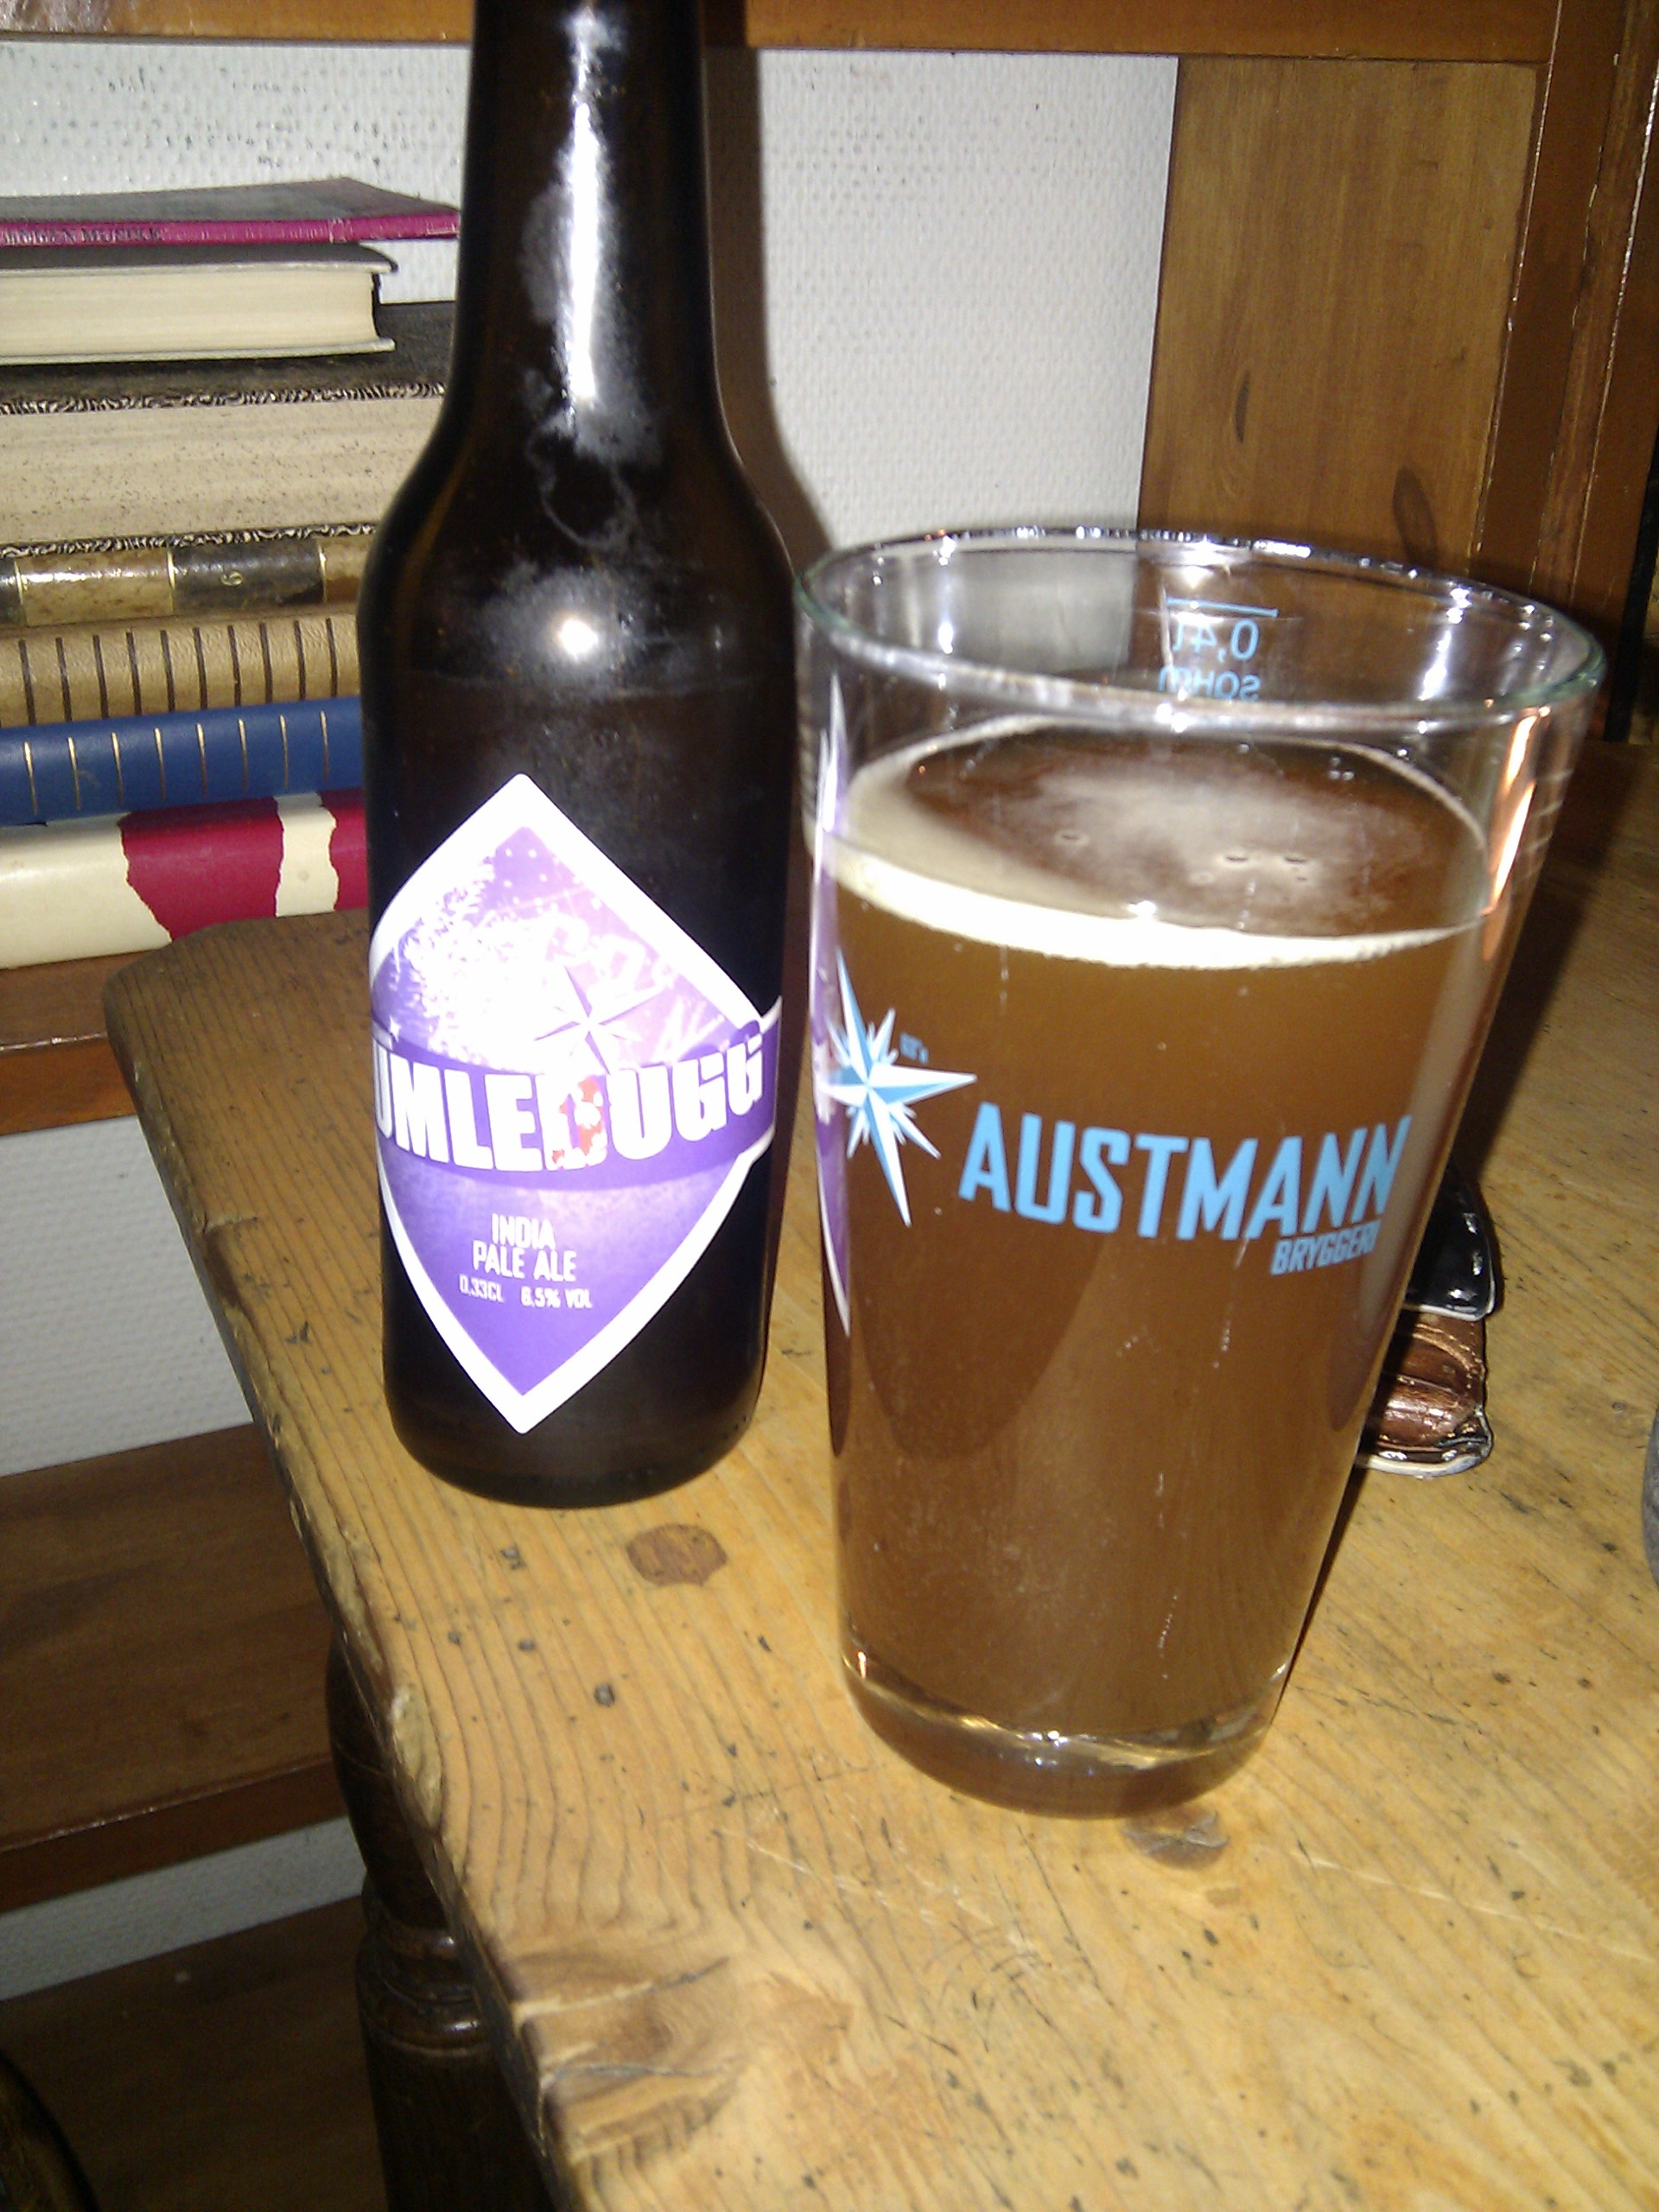
\includegraphics[scale=0.1, angle=0]{Bilder/Ol/humledugg.jpg}
\caption{Humledugg fra "Austmann Bryggeri"}
\end{figure}

\newpage
\subsubsection{Thwaites: Indus Pale Ale}
\paragraph{Kommentar:} Igjen så må jeg bare si KJEDELIG! Har hatt skikkelig uflaks med hvilke øl jeg har kjøpt i det siste. Det er ikke noe galt med smaken og det glir ned som bare det, men det bare så lite smak. Føles som å drikke en lett sommerpils som ikke er det jeg vil ha når jeg kjøper en IPA. Hvis du vil ha en forfriskende IPA til solvarmen så vil denne funke, men hvorfor ikke gå for en pils da?
\newline
-- -- Isak 11.05.2014

\begin{figure} [H]
\centering
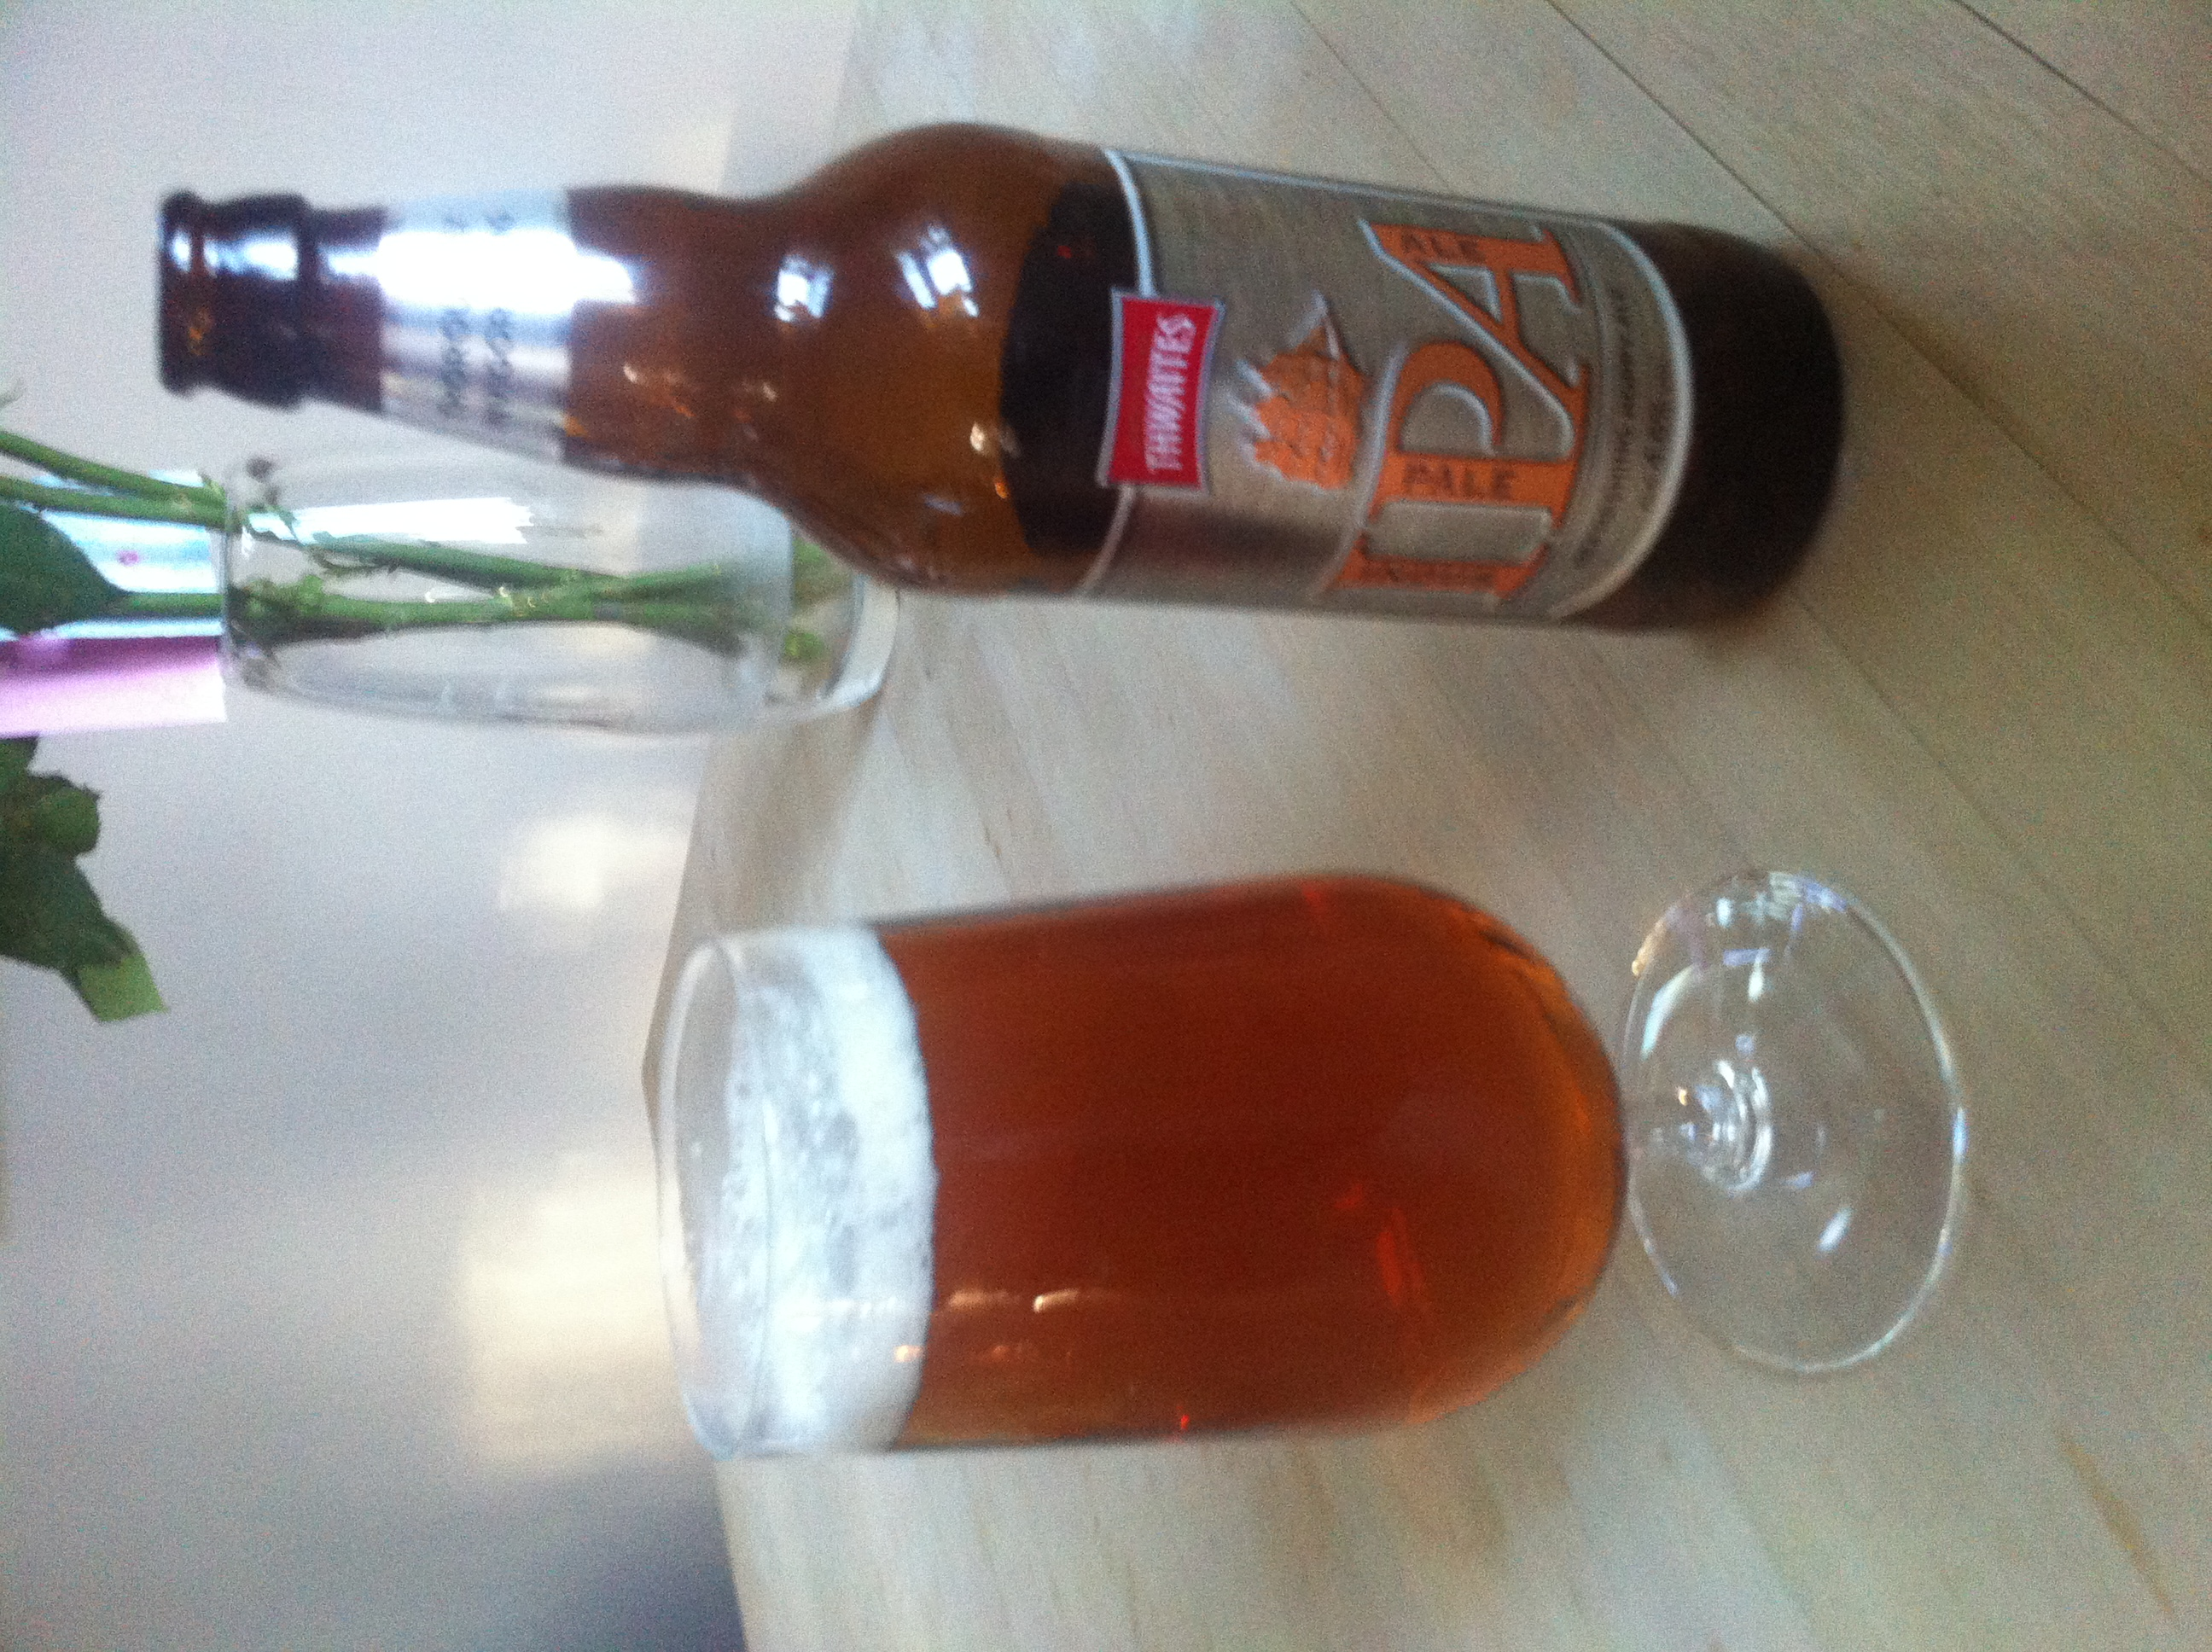
\includegraphics[scale=0.1, angle=270]{Bilder/Ol/ThwaitesIndusPaleAle.jpg}
\caption{Indus Pale Ale fra "Thwaites"}
\end{figure}

\newpage
\subsubsection{Nøgne Ø: Two Captains}
\paragraph{Kommentar:} Dette er blant mine favoritt IPA. Den har en rimelig ram smak, ganske tørr og veldig bitter. Anbefaler alle å prøve denne ved anledning. 
\newline
-- -- Anders 6.08.2014

\begin{figure} [H]
\centering
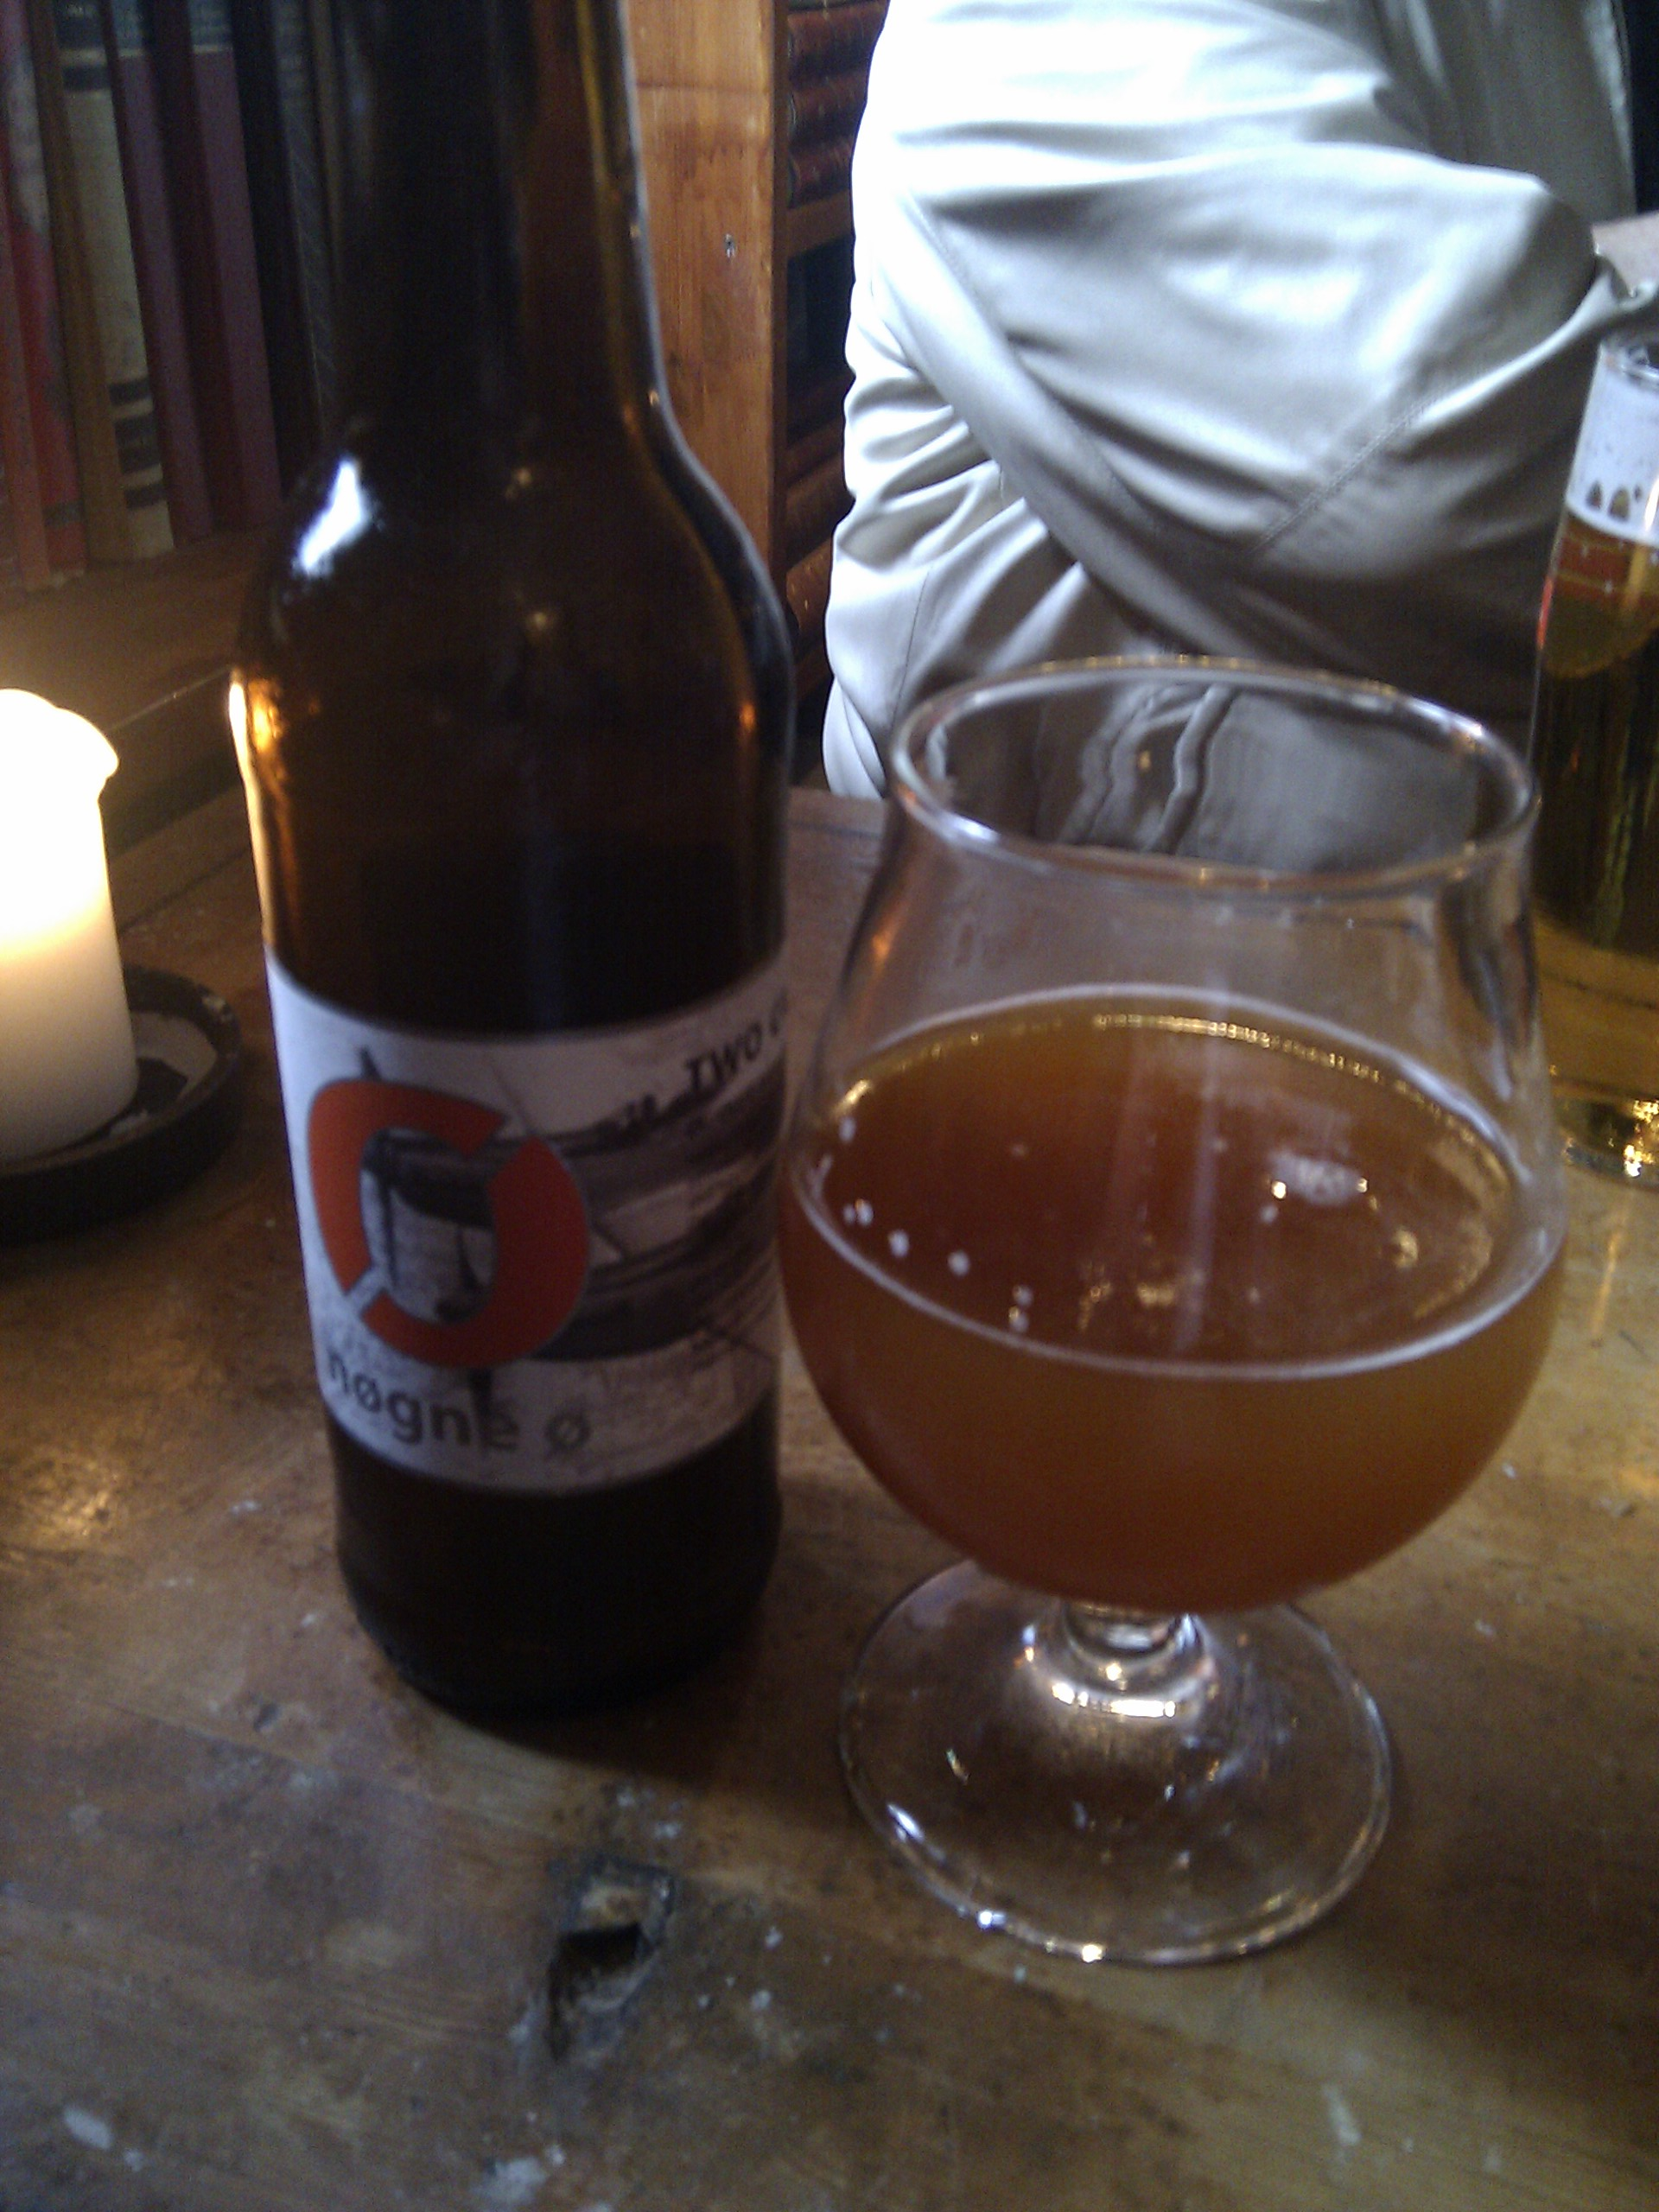
\includegraphics[scale=0.1, angle=0]{Bilder/Ol/twoCpt.jpg}
\caption{Two Captains fra "Nøgne Ø"}
\end{figure}

\newpage
\subsubsection{Boulevard Brewing Co.: Double-Wide I.P.A.}
\paragraph{Kommentar:} Denne var fantastisk bra. Anbefaler alle å prøve den. Om jeg skulle sette fingeren på noe måtte det være at den kunne vært litt mer bitter. Den hadde en litt søt undertone som for meg var noe uvant i en IPA, men dette funket svært bra.
\newline
-- -- Anders 4.10.2014

\begin{figure} [H]
\centering
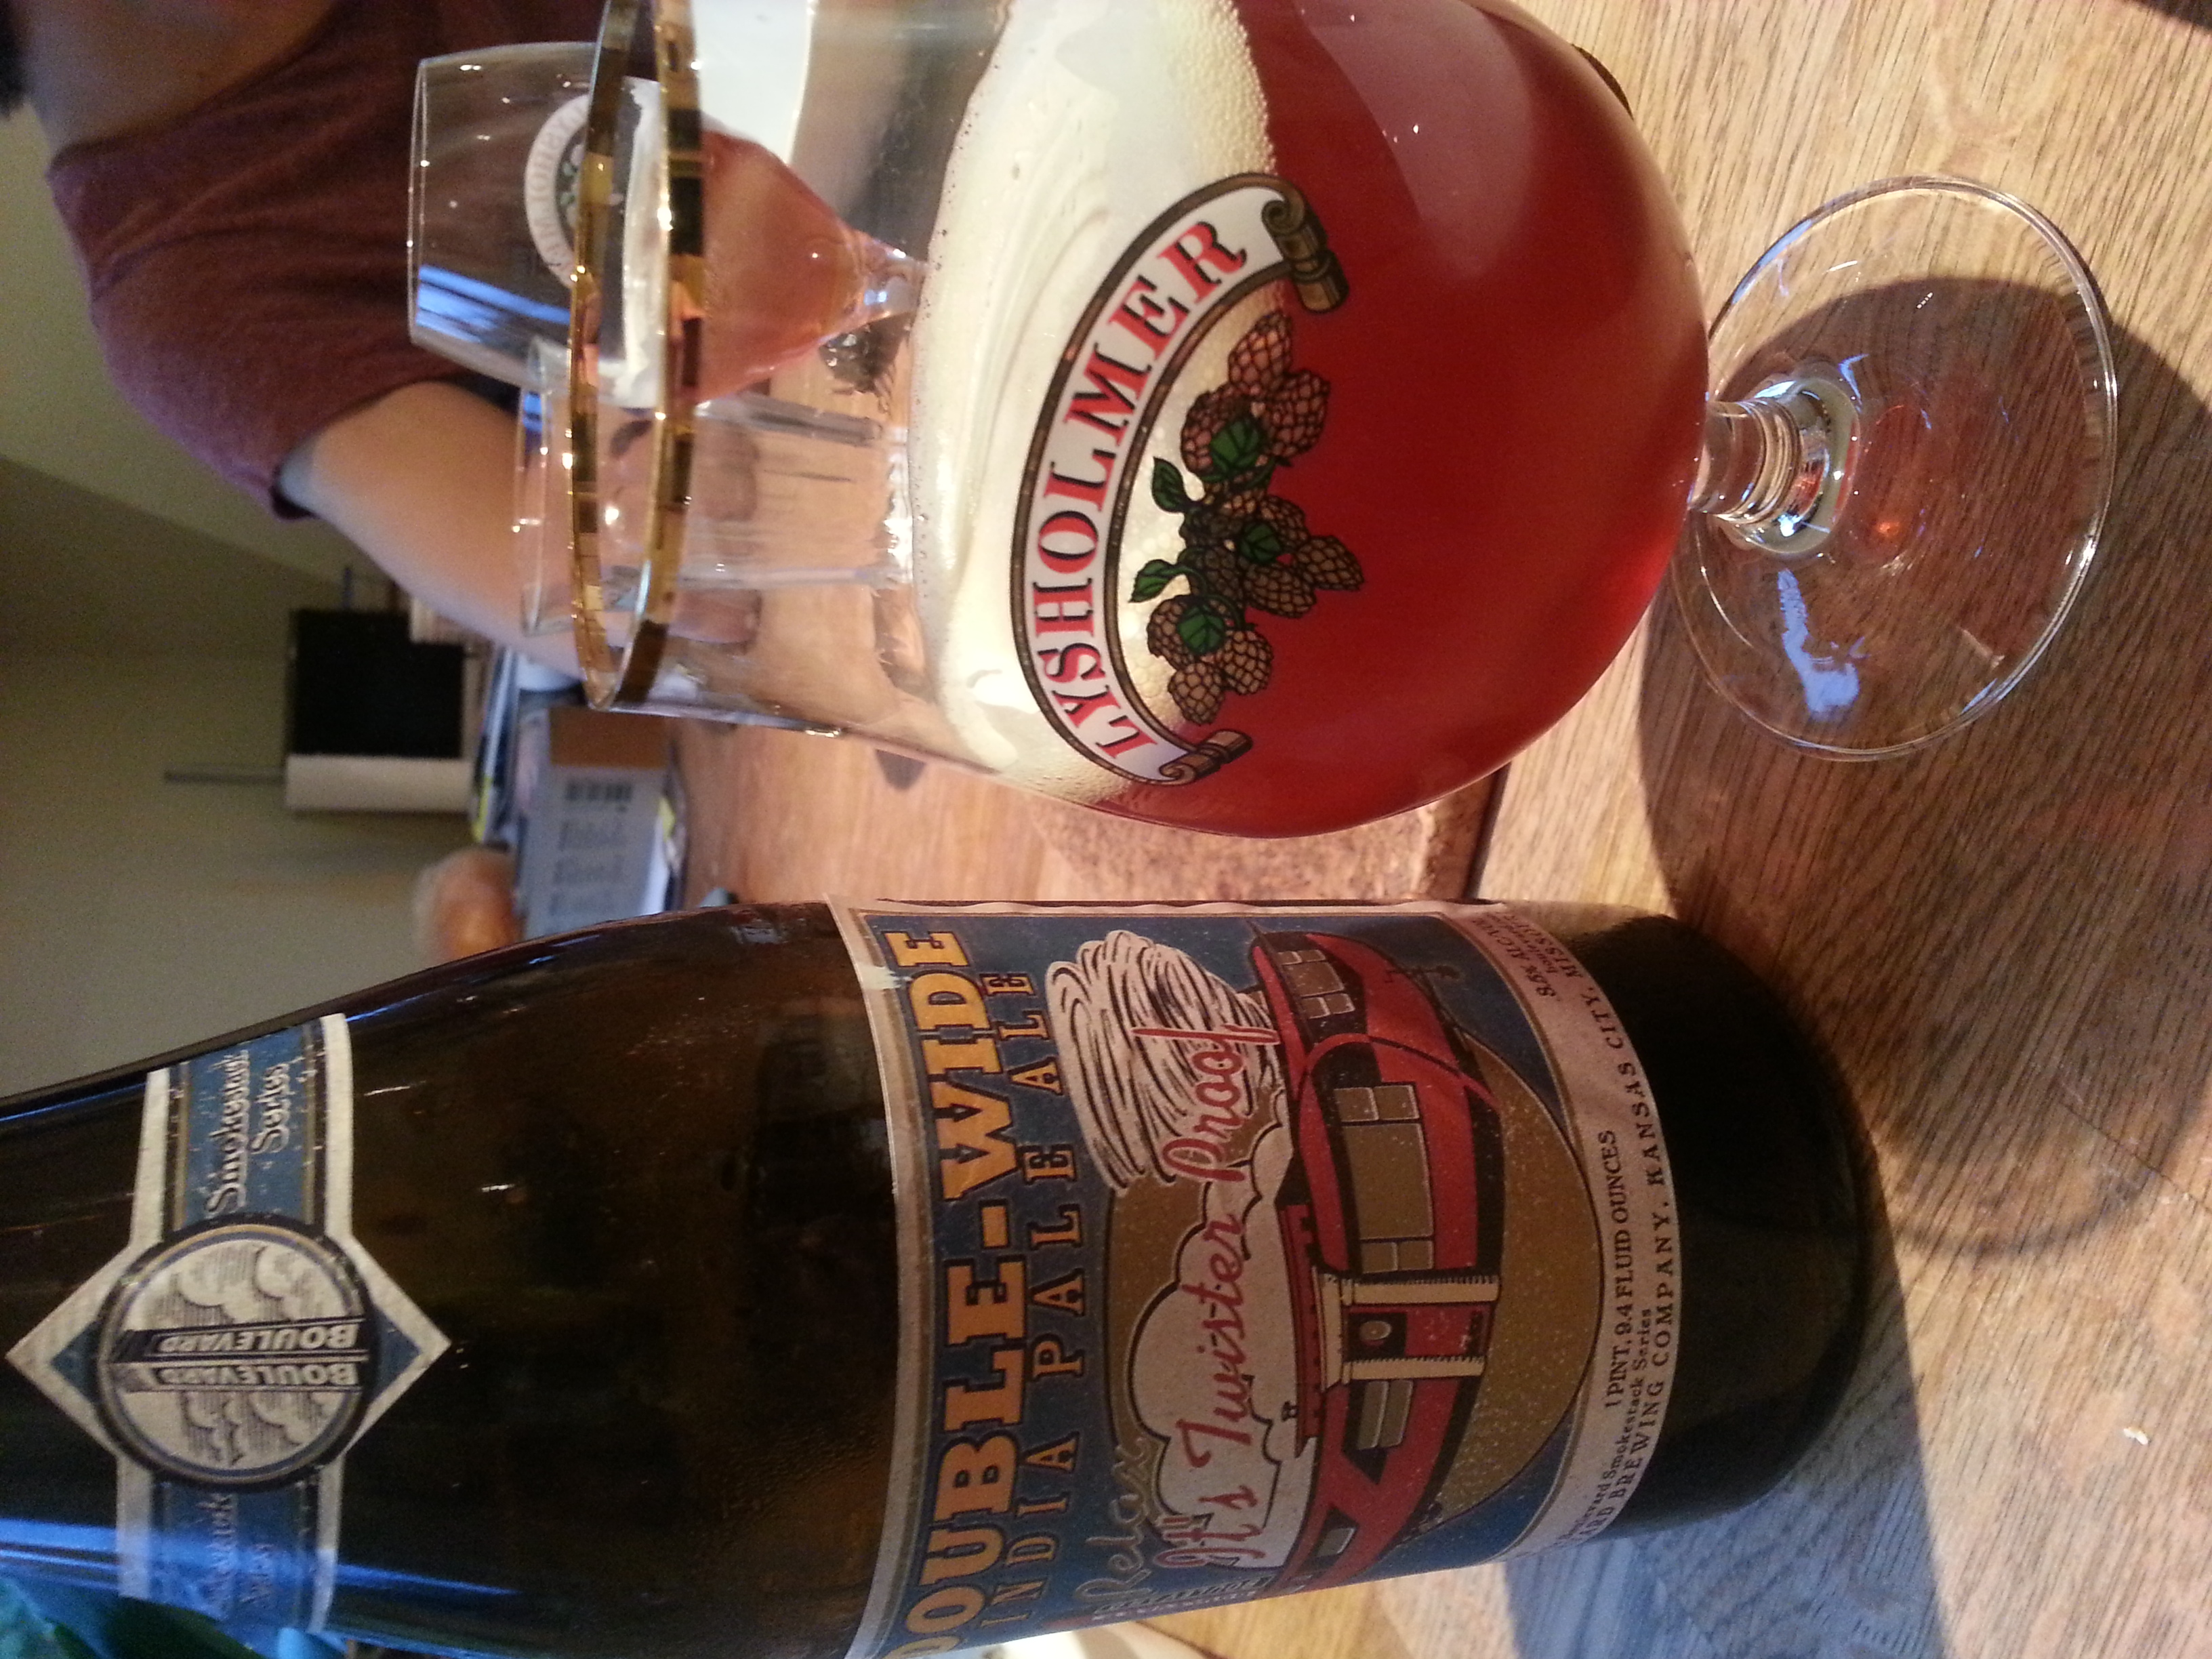
\includegraphics[scale=0.1, angle=270]{Bilder/Ol/Double-Wide.jpg}
\caption{Double-Wide I.P.A. fra "Boulevard Brewing Co."}
\end{figure}

\newpage
\subsubsection{Øystein Kvalvaag Hjemmebrygg: Kvalvaag IPA}
\paragraph{Kommentar:} En studie av bygdefest anno 2014. Lørdag 05.10.2014 var vi bedt på bygdefest på Bakketun (i nærheten av Kvalvaag). Anledningen var ett 50-årslag. Frekvensen av dressjakke, t-skjorte, jeans og sylspisse pub til pub sko var akkurat som forventet på bygdefest. Hårsveiser fra 70-tallet og flatfyll var også som forventet. Men det som overasket mektig var maten (som var noe av det beste jeg har smakt) og øllet som også hadde meget høy kvalitet. Kvalvaag IPA er en standard, men veldig god IPA. Hadde du fått den servert på pub så hadde du tenkte at det var en god om dog ikke ekstraordinær IPA. Litt på den lyse siden av IPA.
-- -- Isak 05.10.2014

\begin{figure} [H]
\centering
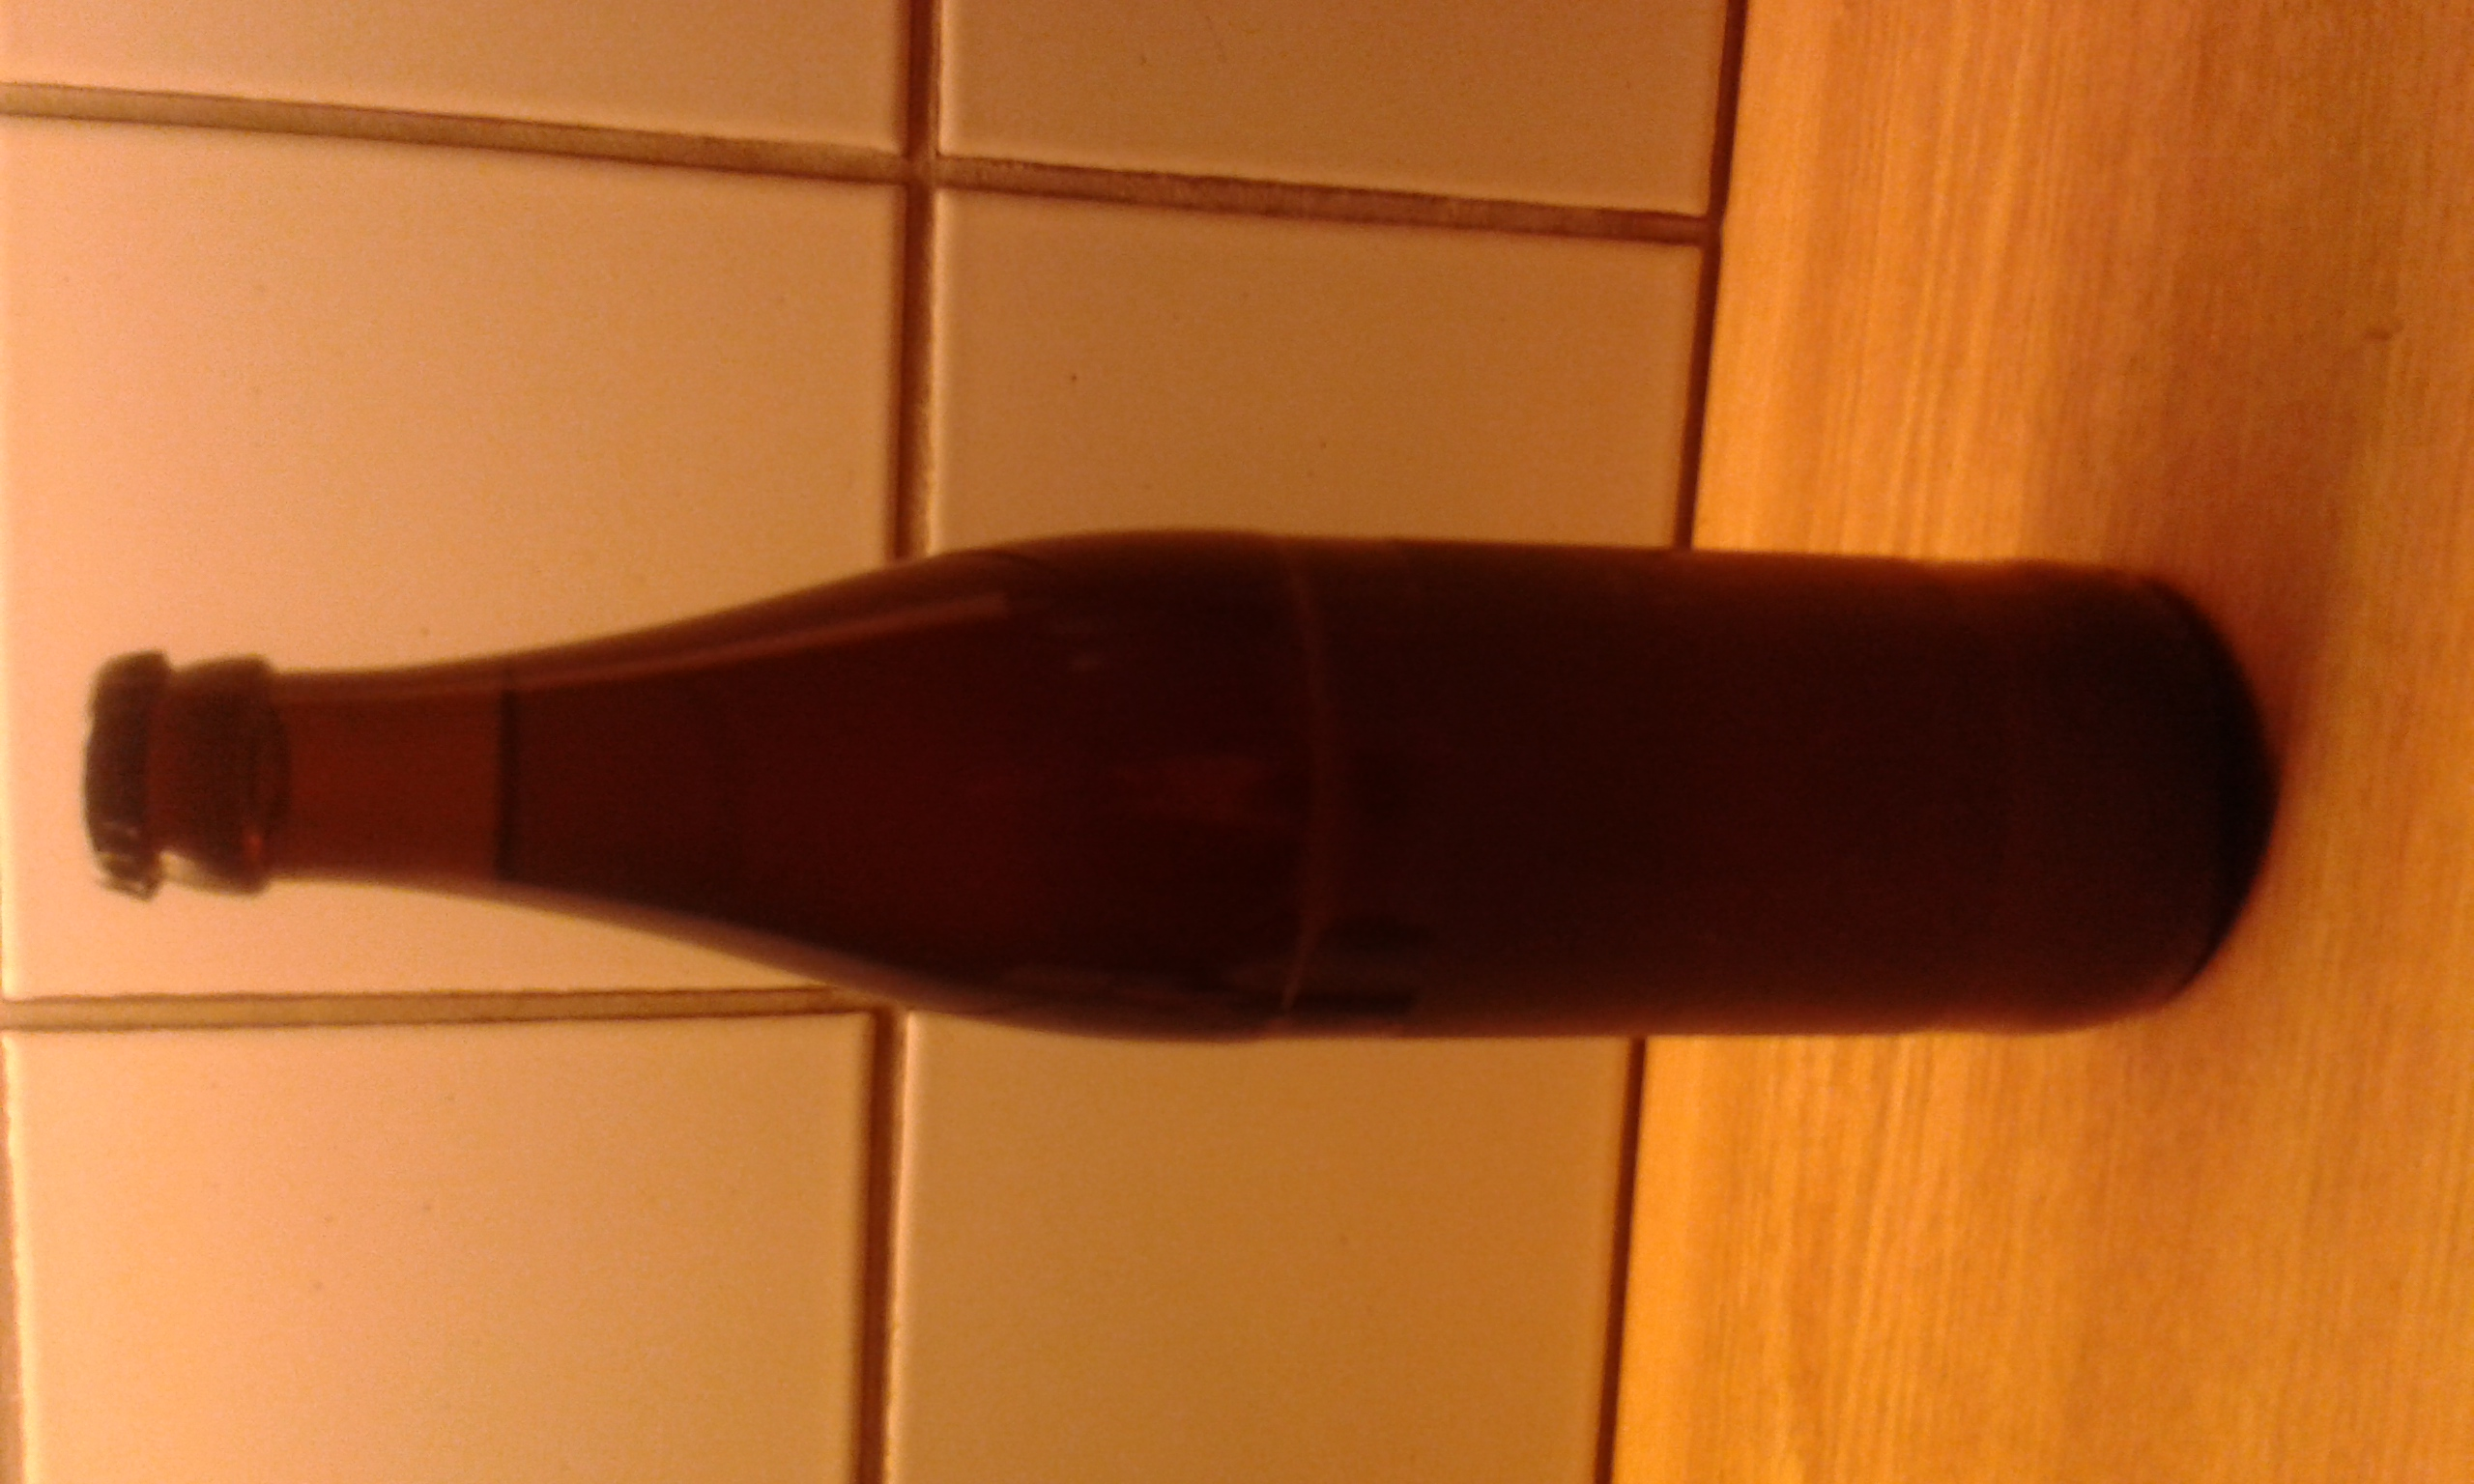
\includegraphics[scale=0.1, angle=270]{Bilder/Ol/KvalvaagIPA}
\caption{Kvalvaag IPA fra "Øystein Kvalvaag Hjemmebryggeri"}
\end{figure}

\newpage
\subsection{Pale Ale}
\subsubsection{HaandBryggeriet: Pale Ale}
\paragraph{Kommentar:} En av det beste øl jeg har smakt på lenge. God og fyldig med masse smak. En prefekt balanse mellom en rik smak samtidig som den er lettdrikkelig. Spiste den sammen med en Tikka Masala gryte og dette er en øl som går godt til mat eller for seg selv.
\newline
-- -- Isak 04.06.2014

\begin{figure} [H]
\centering
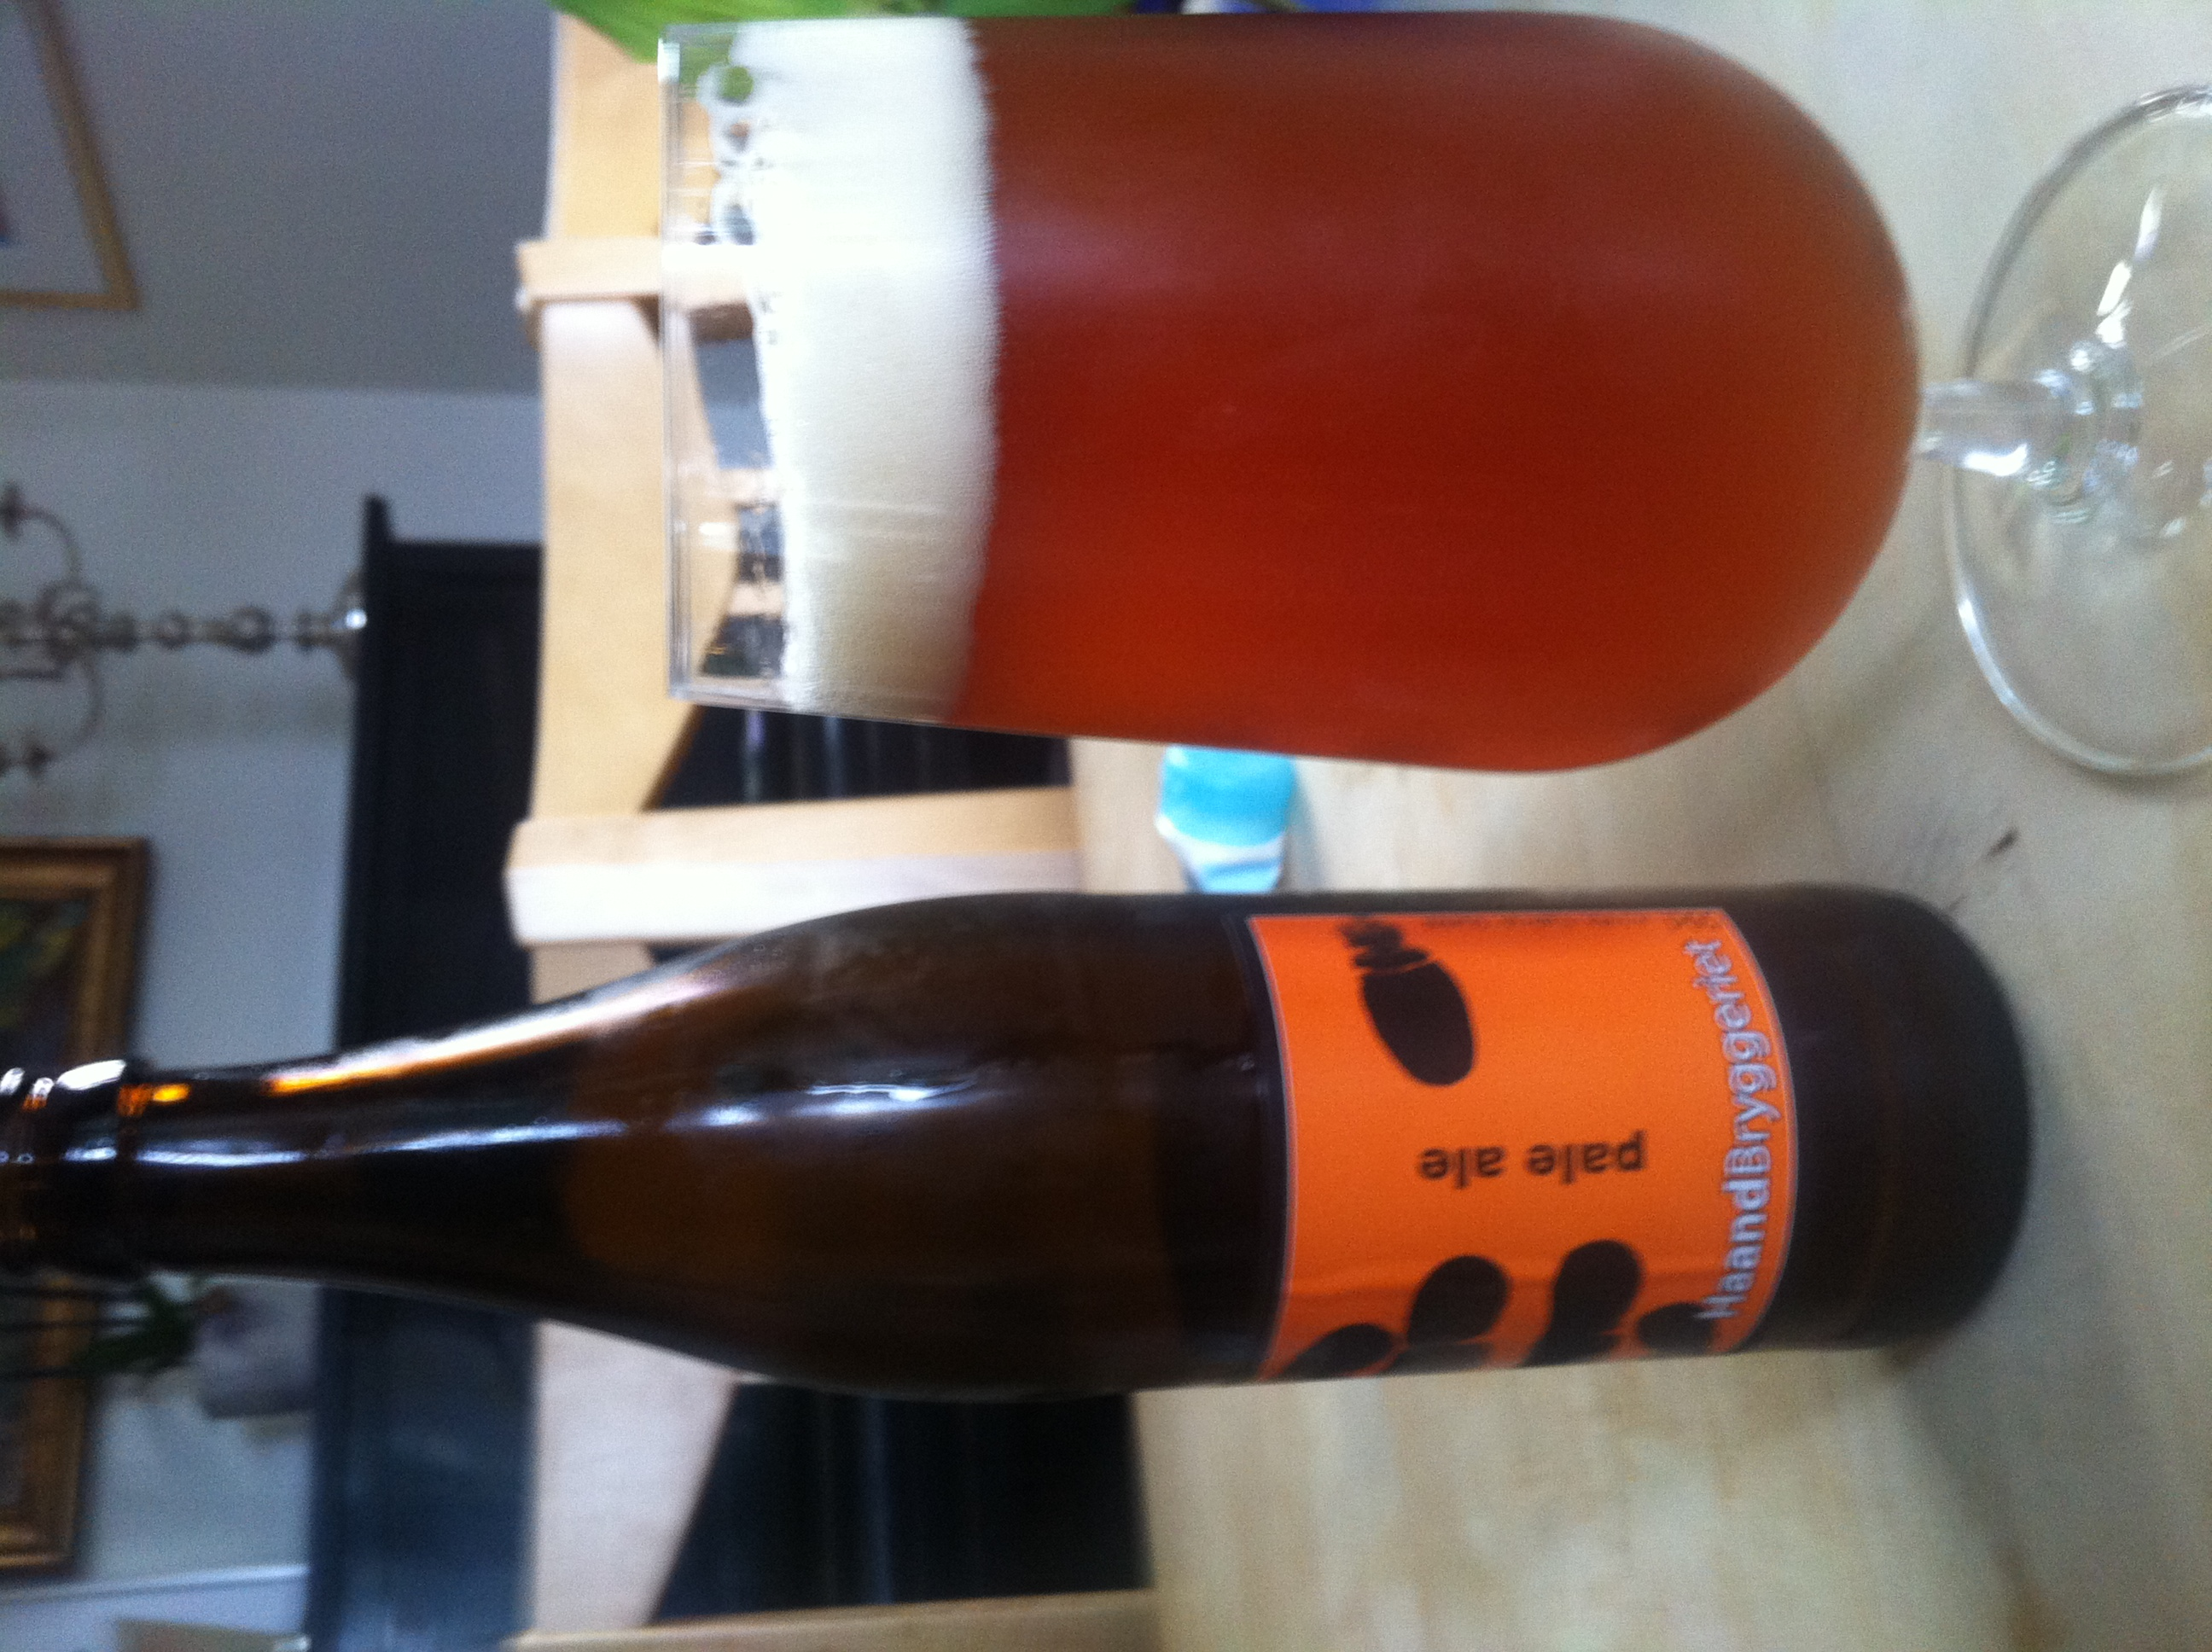
\includegraphics[scale=0.1, angle=270]{Bilder/Ol/palealehaand}
\caption{Pale Ale fra HaandBryggeriet}
\end{figure}

\newpage
\subsection{Hveteøl}
\subsubsection{Ægir Bryggeri: Witbier}
\paragraph{Kommentar:} Til å være hveteøl var denne mindre søt enn jeg hadde forventet. Den var lett og lys, og egner seg kanskje i mer sommerlige situasjoner enn jeg drakk den i. Selv savnet jeg litt mer ramm smak, men det skal man kanskje ikke forvente av en hveteøl. Hadde jeg hatt valget mellom denne og en Dahls ville jeg tatt denne, så lenge jeg ikke måtte betale for den selv. For lite smak for pengene rett å slett.
\newline
-- -- Anders 14.04.2014

\begin{figure} [H]
\centering
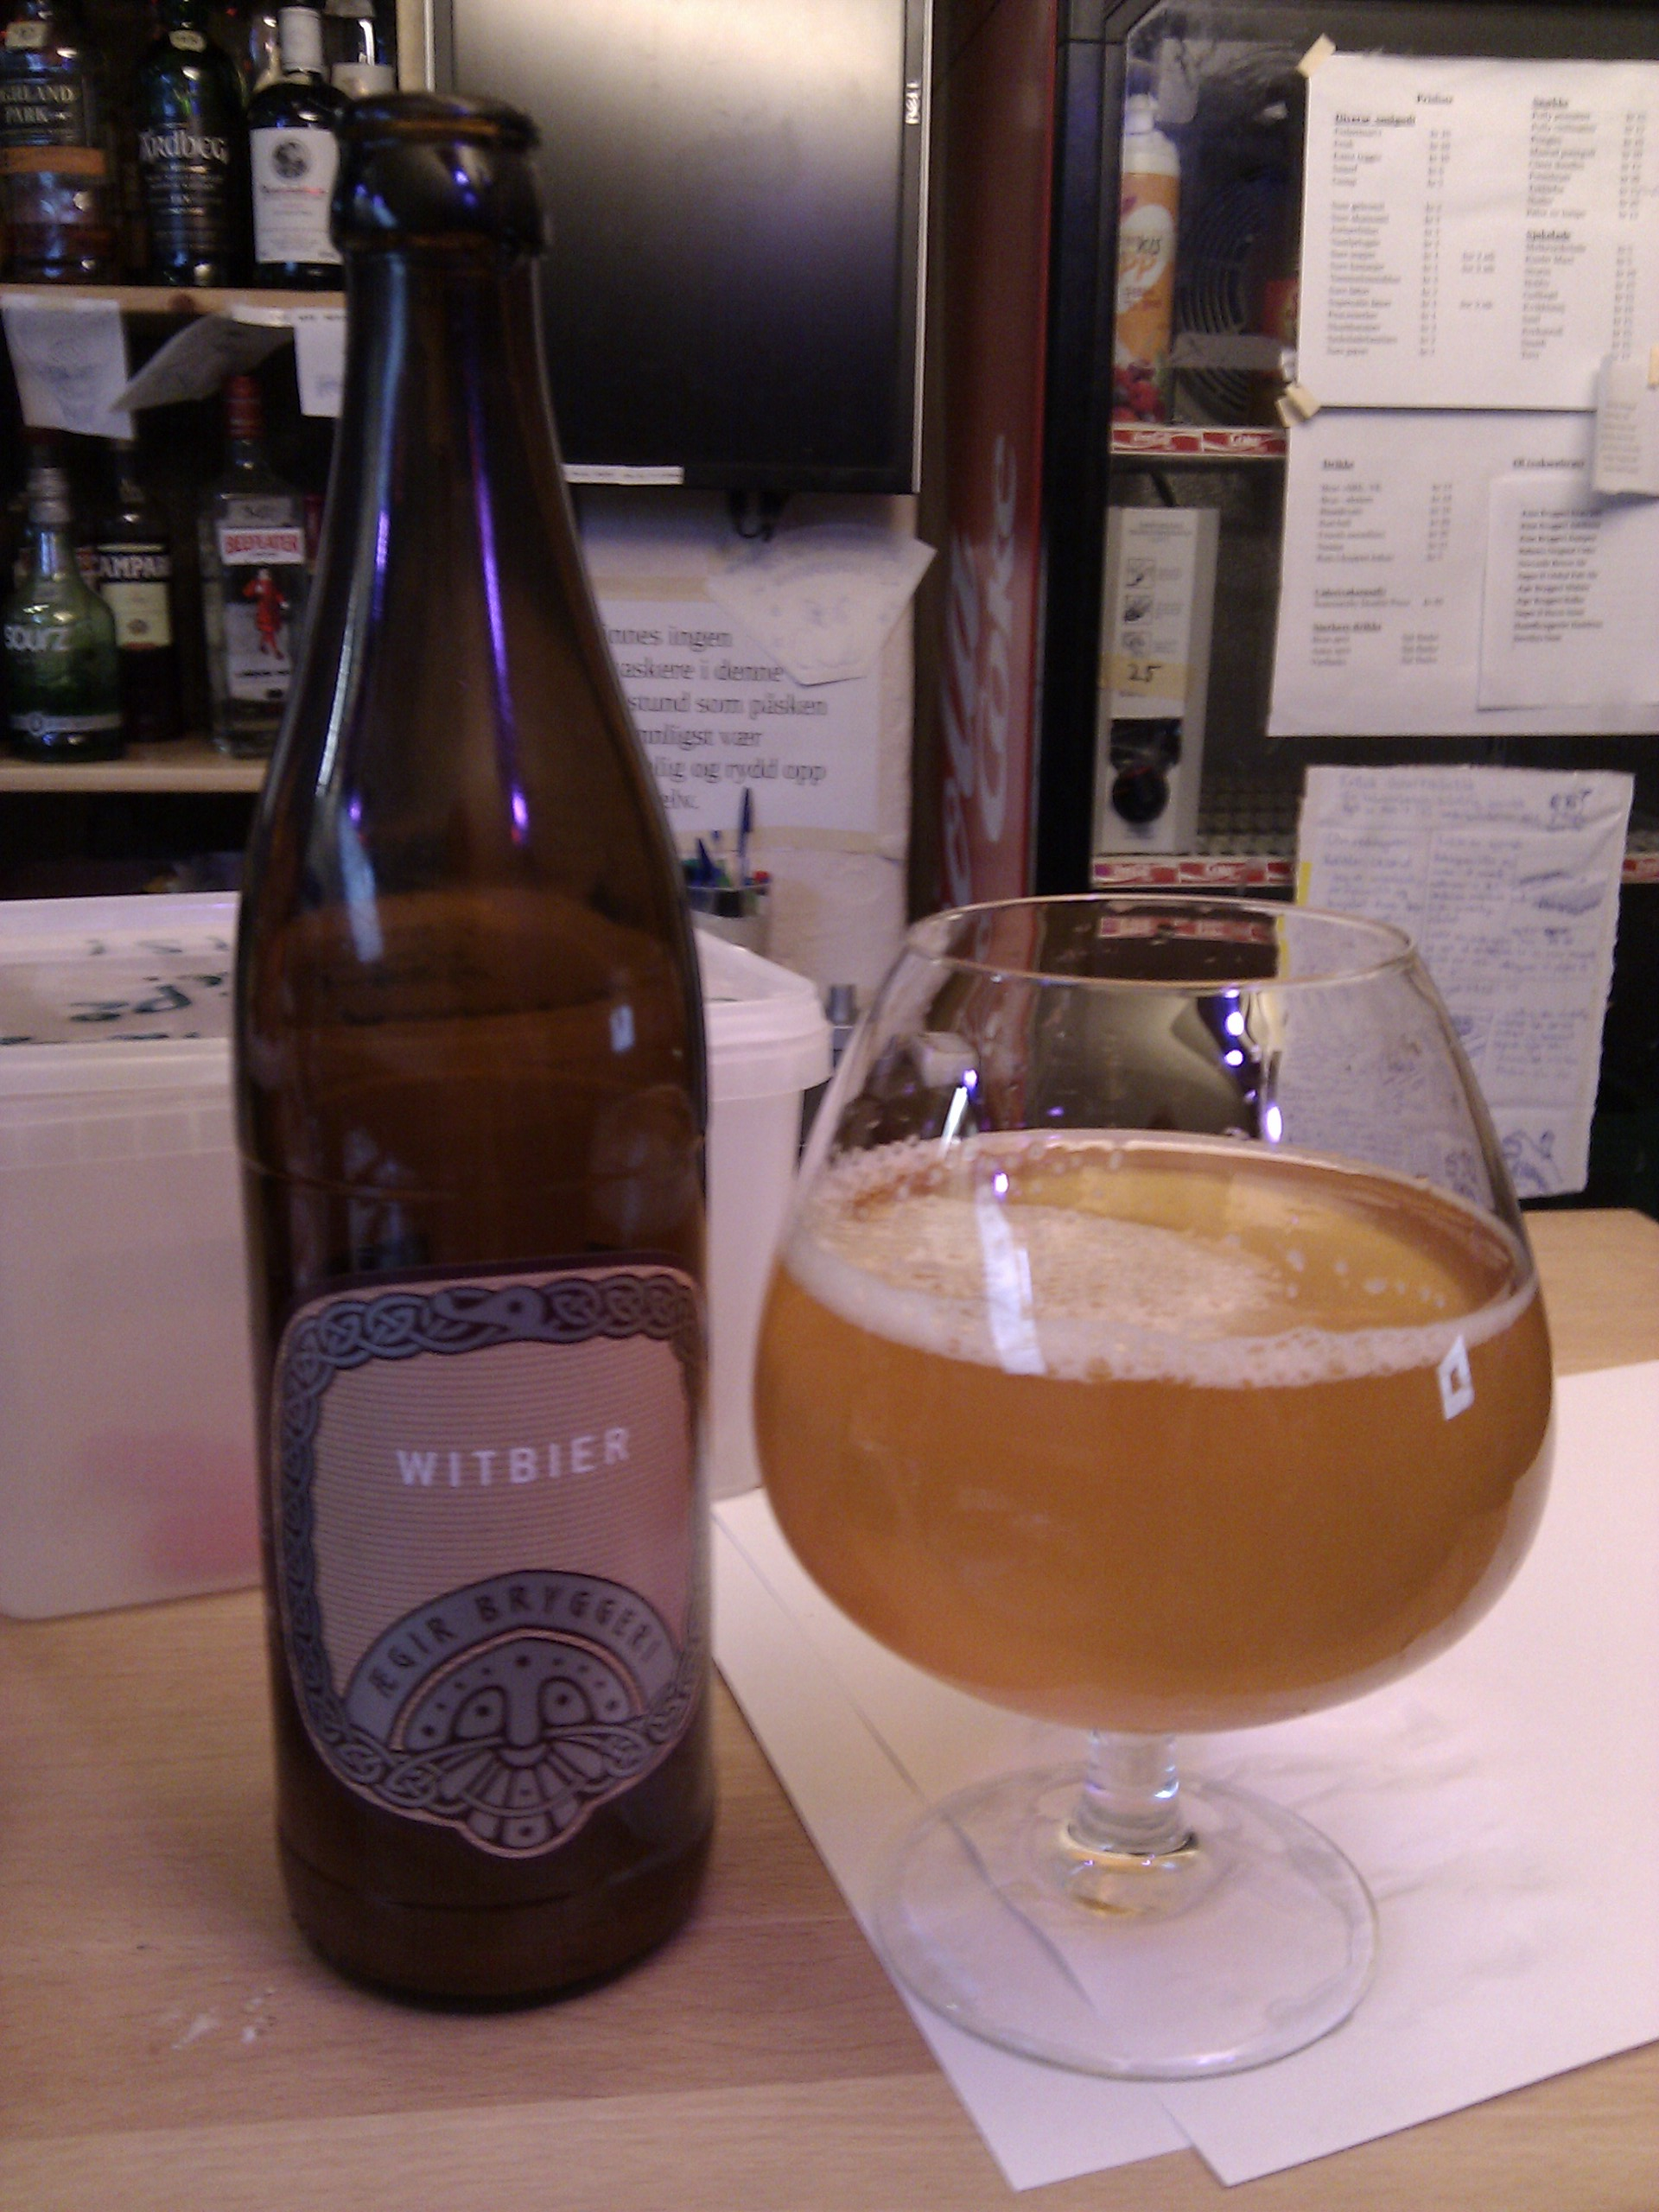
\includegraphics[scale=0.1, angle=0]{Bilder/Ol/EgirBryggeriWitbier.jpg}
\caption{Witbier fra "Ægir Bryggeri"}
\end{figure}

\newpage
\subsection{Lager}
\subsubsection{Grupo Empresarial Bavaria: Cerveza Aguila}
\paragraph{Kommentar:} Nok et eksempel på at jeg bør gjøre litt mer reaserch før jeg prøver nye øl. Hvis man søker på Cerveza Aguila så får man opp masse promoteringsbilder av lettkledde strandbabes i bikini, med Aguila trykket strategisk i byste- og stussområde. Dette er en øl som er ment å nytes på samme måte som en Corona og det merker man på den lette enkle smaken. En helt grei øl for hva det er ment som, men når man betaler importøl pris på den og egentlig er ute etter noe mer spennende så blir det litt skuff. 
\newline
-- -- Isak 11.05.2014

\begin{figure} [H]
\centering
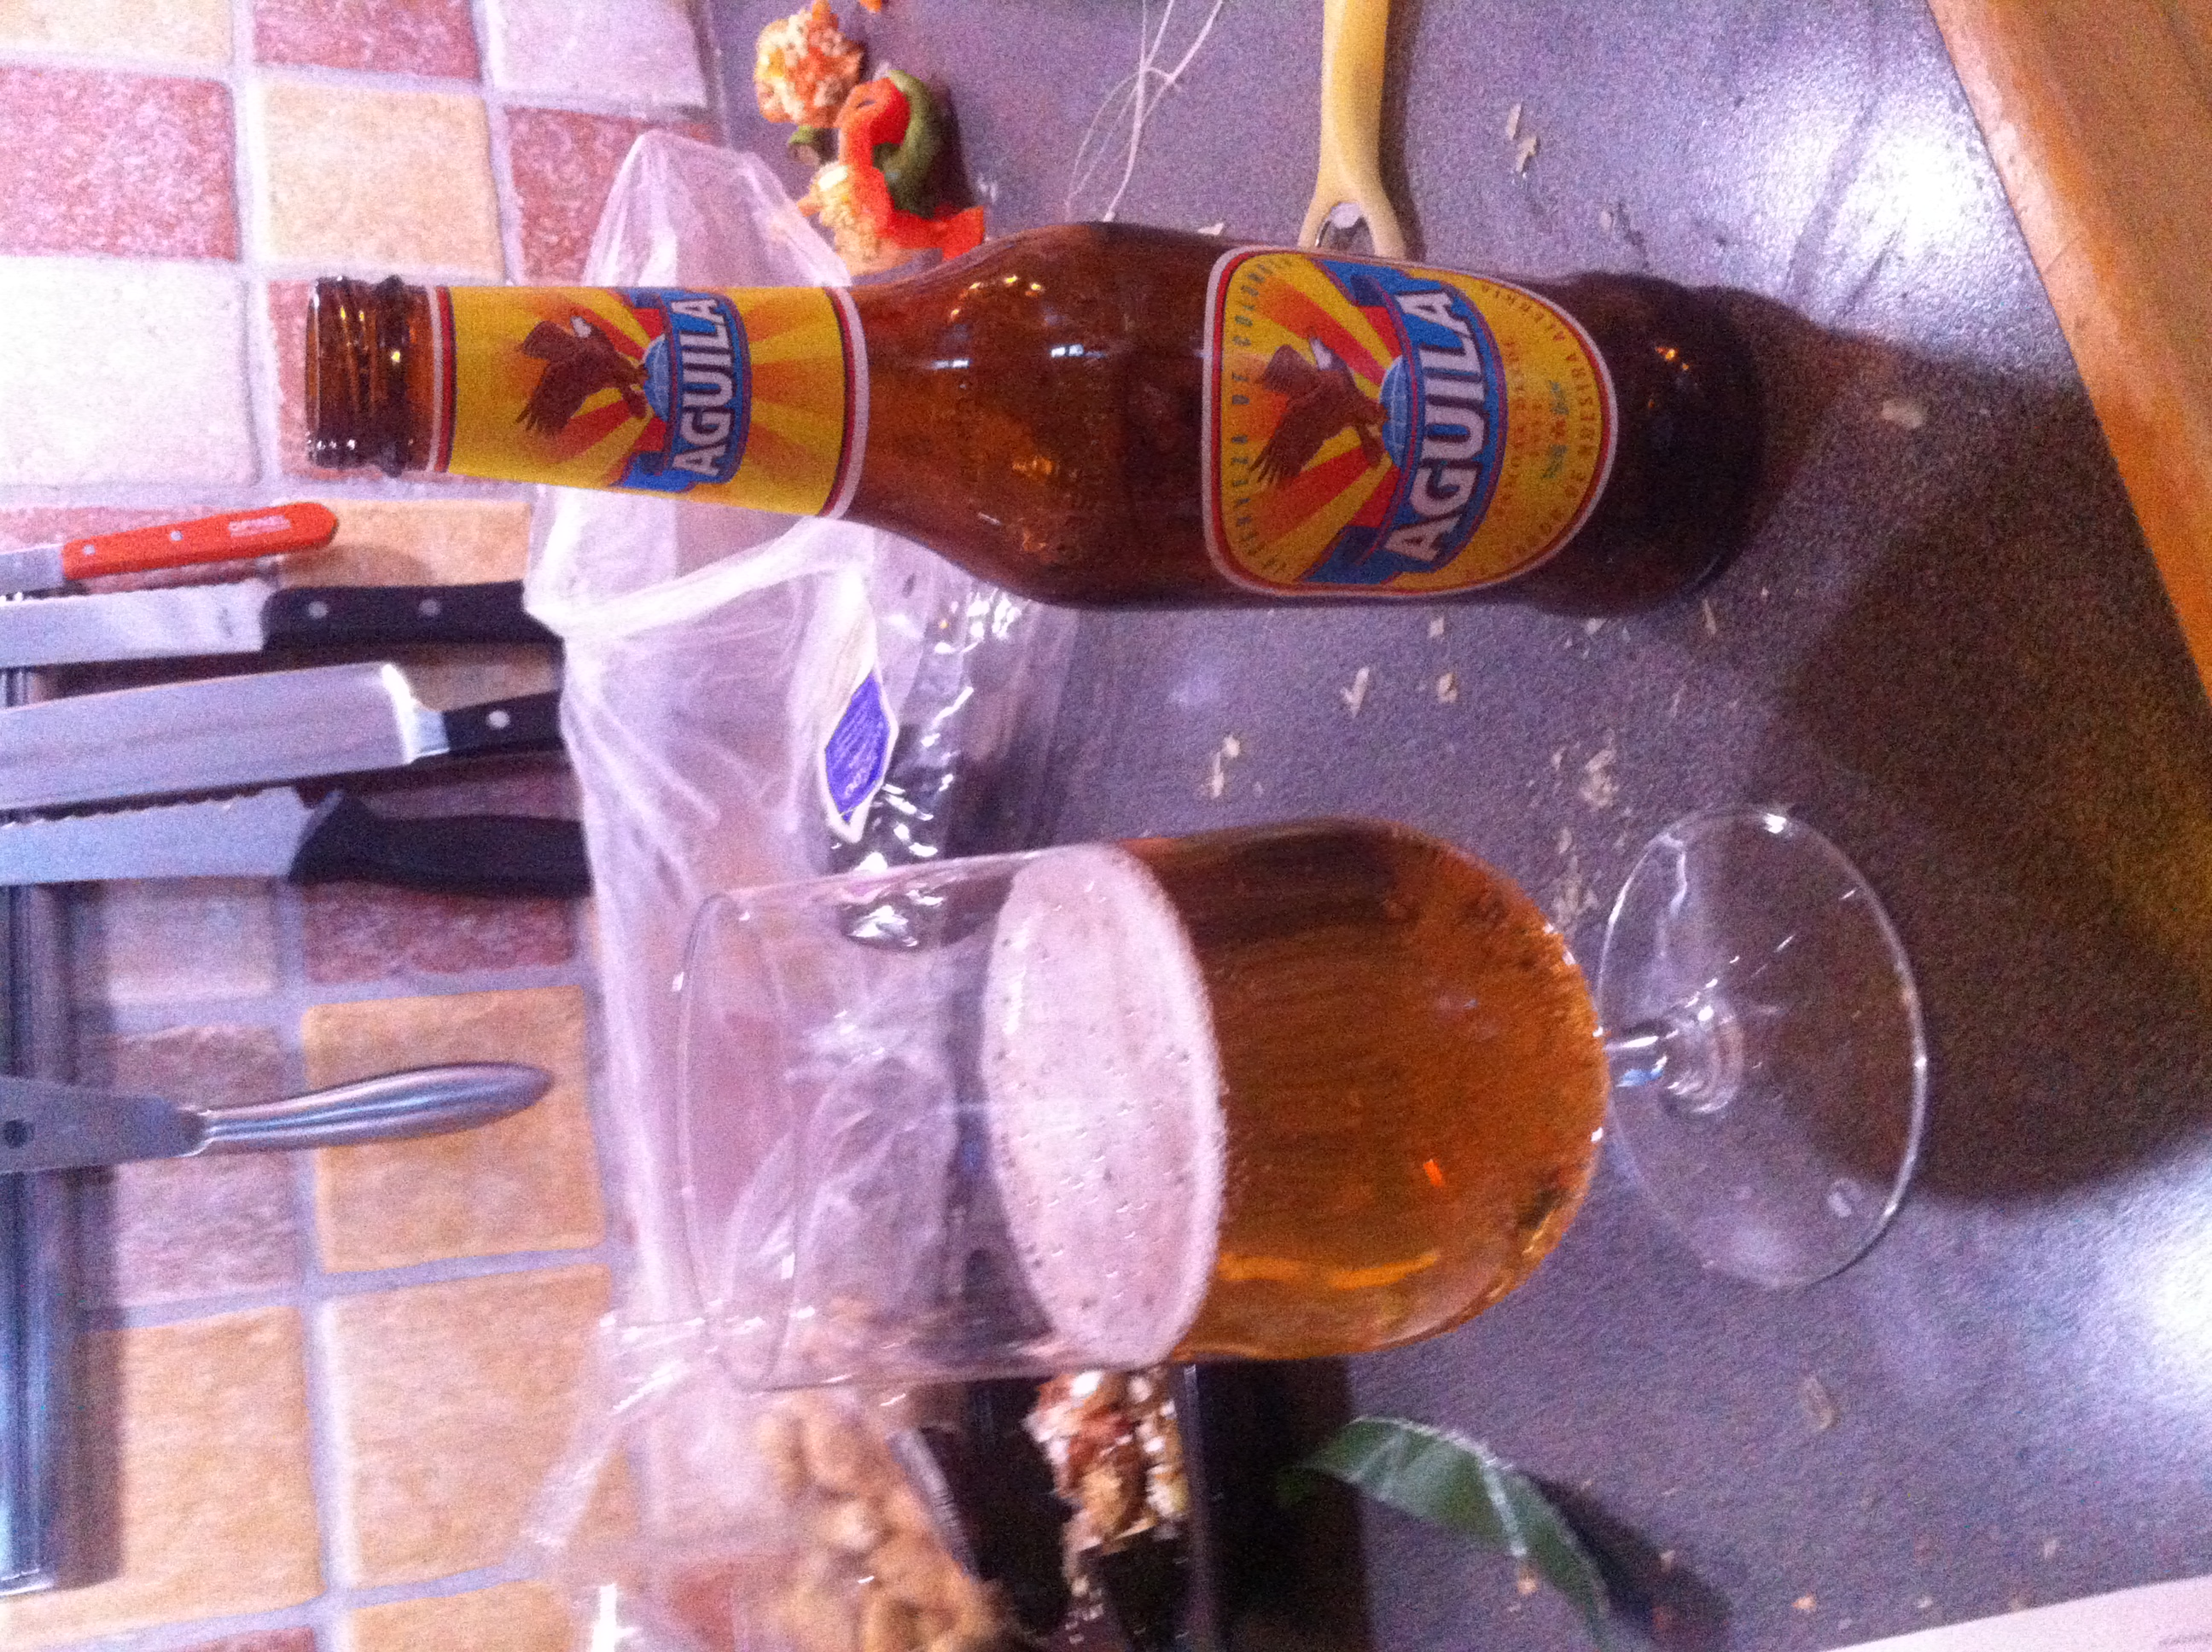
\includegraphics[scale=0.08, angle=270]{Bilder/OL/CervezaAguila.jpg}
\caption{Cerveza Aguila fra "Grupo Empresarial Bavaria"}
\end{figure}   

\begin{figure} [H]
\centering
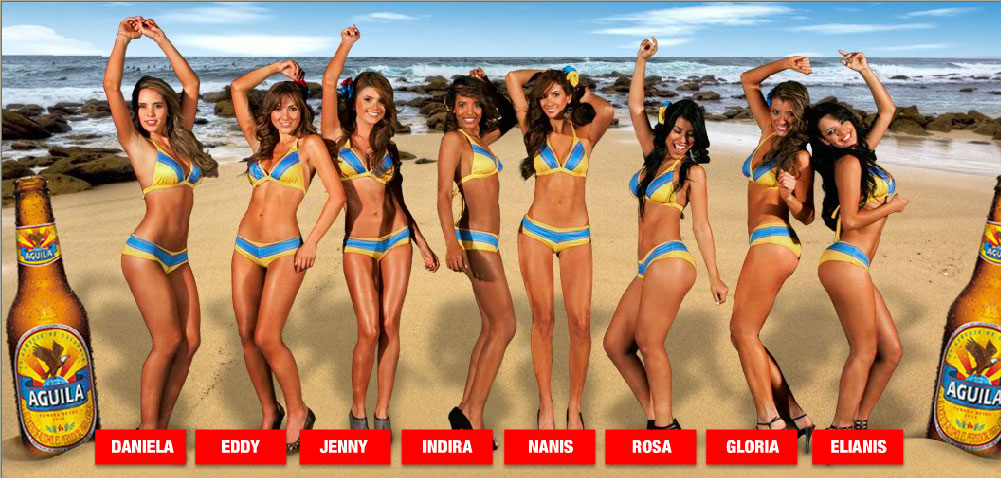
\includegraphics[scale=0.31, angle=0]{Bilder/OL/chicas-aguila-2011.jpg}
\caption{Babes fra "Grupo Empresarial Bavaria" a-yeah --Anders}
\end{figure}  

\newpage
\subsection{Stout}
\subsubsection{Boulevard Brewing Company: Dark Truth Stout}
\paragraph{Kommentar:} Nesten ti prosent så det er en litt sjokkartet opplevelse å ta de to første slurkene. Selv om det ikke er en veldig stor flaske så går den rett i fletta hvis du ikke har mat i magen fra før. Hvis du liker øl med høy alkoholprosent og du liker mørkt øl så er den en veldig god når du blir vant til den. Mørk og fyldig med masse smak. Passer ypperlig sammen med fet og tung mat. God verdi for pengene. 
\newline
-- -- Isak 07.11.2014

\begin{figure} [H]
\centering
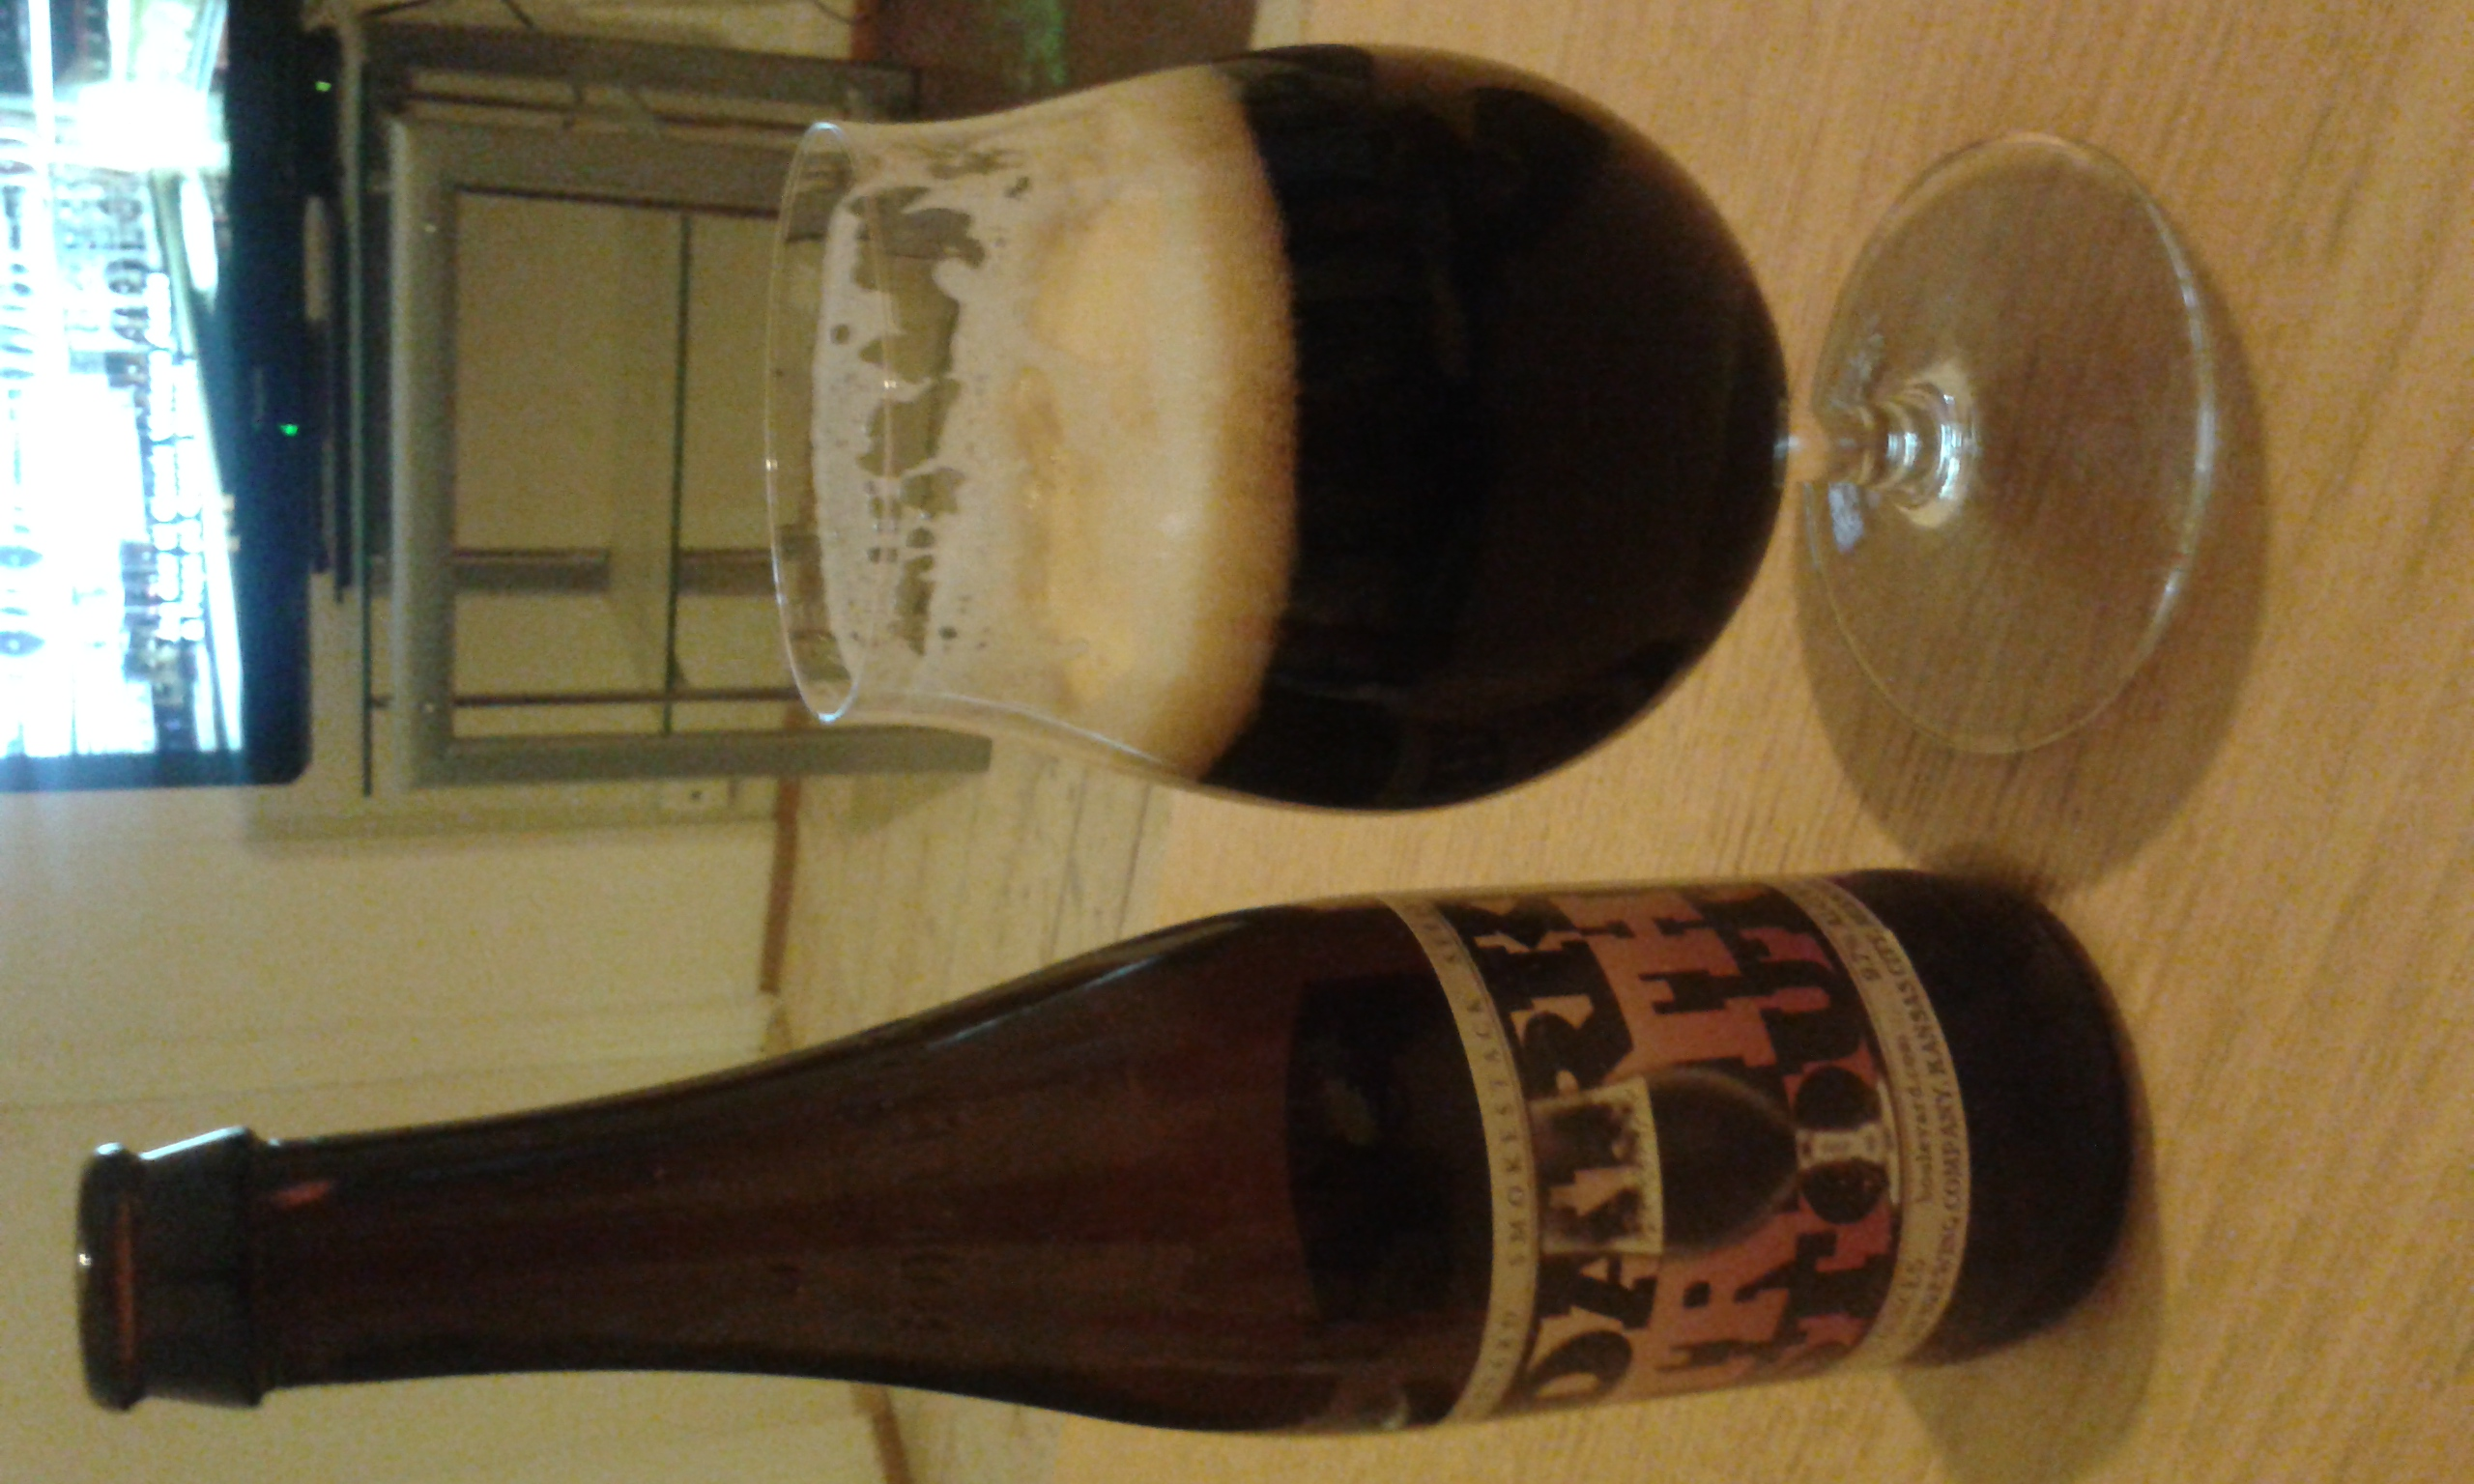
\includegraphics[scale=0.1, angle=270]{Bilder/Ol/darktruthstout}
\caption{Dark Truth Stout fra "Boulevard Brewing Company}
\end{figure}

\newpage
\section{Vin}

\newpage
\section{Sprit}
\subsection{Whisky}
\subsubsection{Lagavulin: Island Single Malt Scotch Whisky 16 Years}

\paragraph{Kommentar:}Sterk, men behagelig røkpreg. En "varmende" avrunding, men ikke en typisk rund whisky. Til en middels høy pris på polet er dette verdt hver krone. Et må ha i barskapet. Plix ikke bland cola i dette a.
\newline
-- -- Anders 13.04.2014

\begin{figure} [H]
\centering
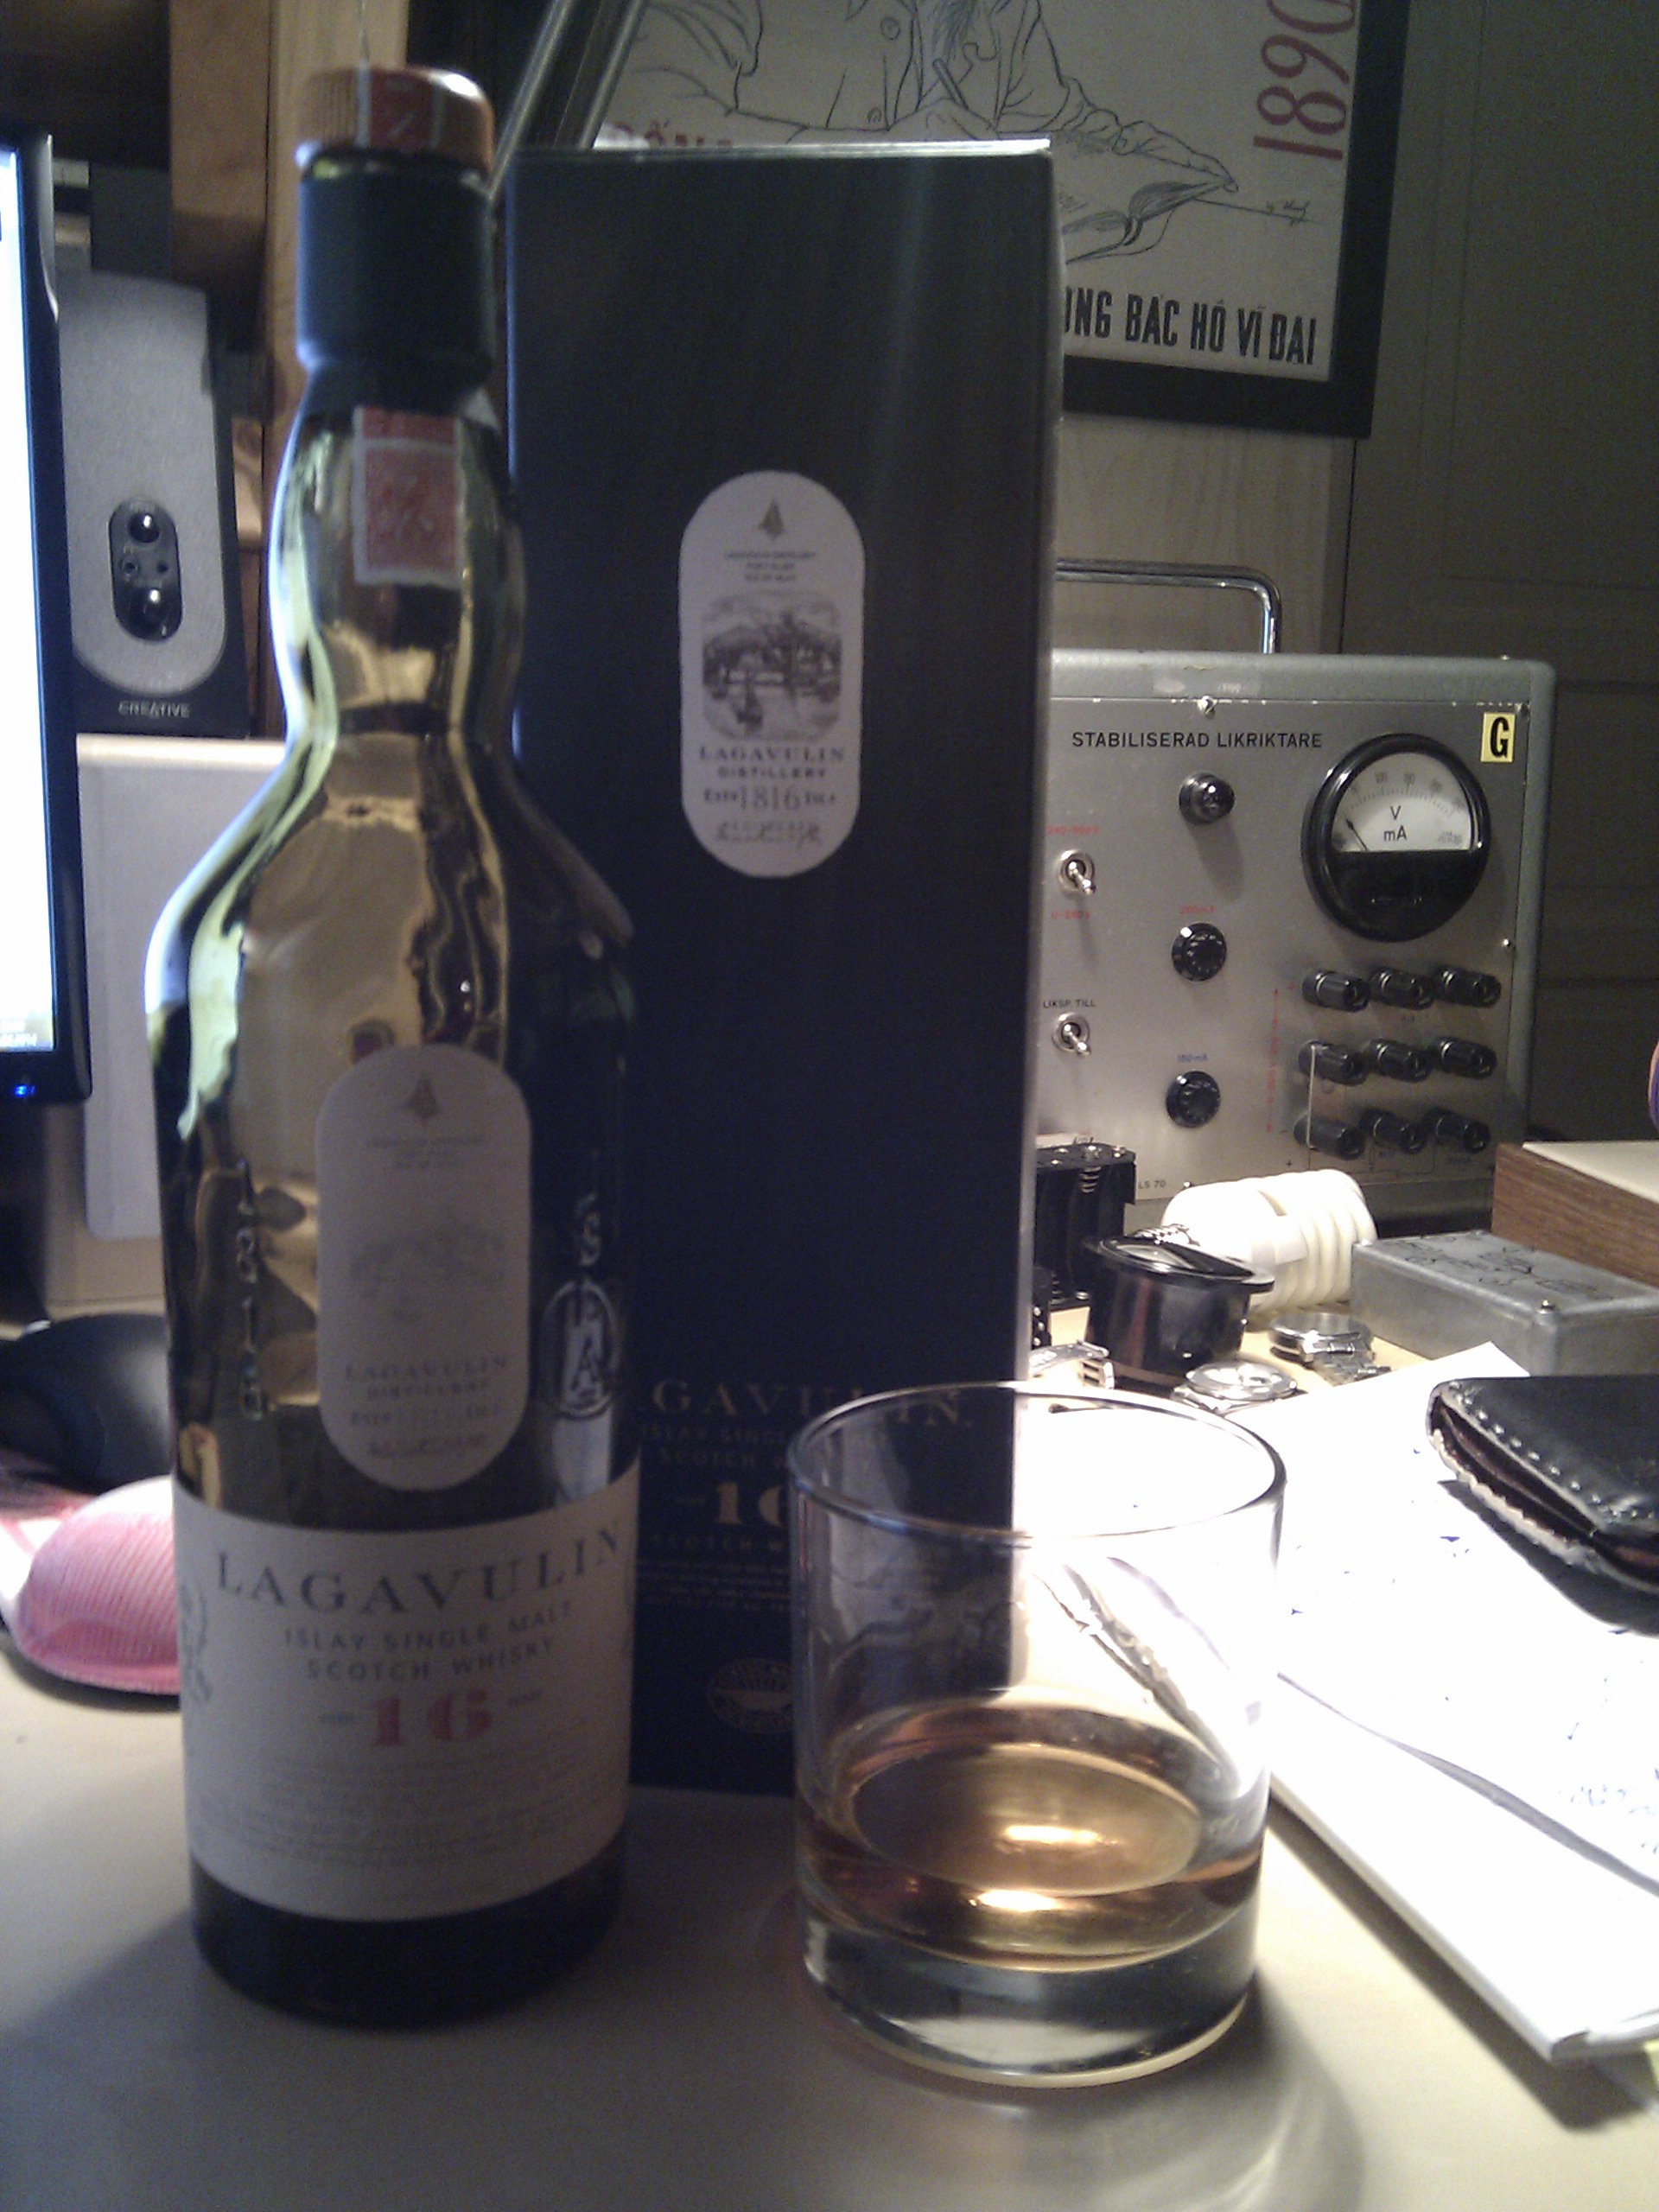
\includegraphics[scale=0.1, angle=0]{Bilder/Sprit/Lagavulin16aar.jpg}
\caption{Island Single Malt Scotch Whisky 16 Years fra "Lagavulin"}
\end{figure}

\newpage
\subsubsection{Highland Park: Thor 16 Years}
\paragraph{Kommentar:} Highland Park er mitt favorittdestilleri og dette er min favoritt noen sinne. Etter min mening har den en perfekt balanse mellom å være full av smak uten å være for kraftig og god og rund uten å være søtlig. Røyksmak, ingefær og ettersmak av vanilje som sitter igjen på en god måte. Noen syns kanskje innpakningen og historien rundt er litt corny, men jeg syns det er bonus. 
\newline
-- -- Isak 11.05.2014

\begin{figure} [H]
\centering
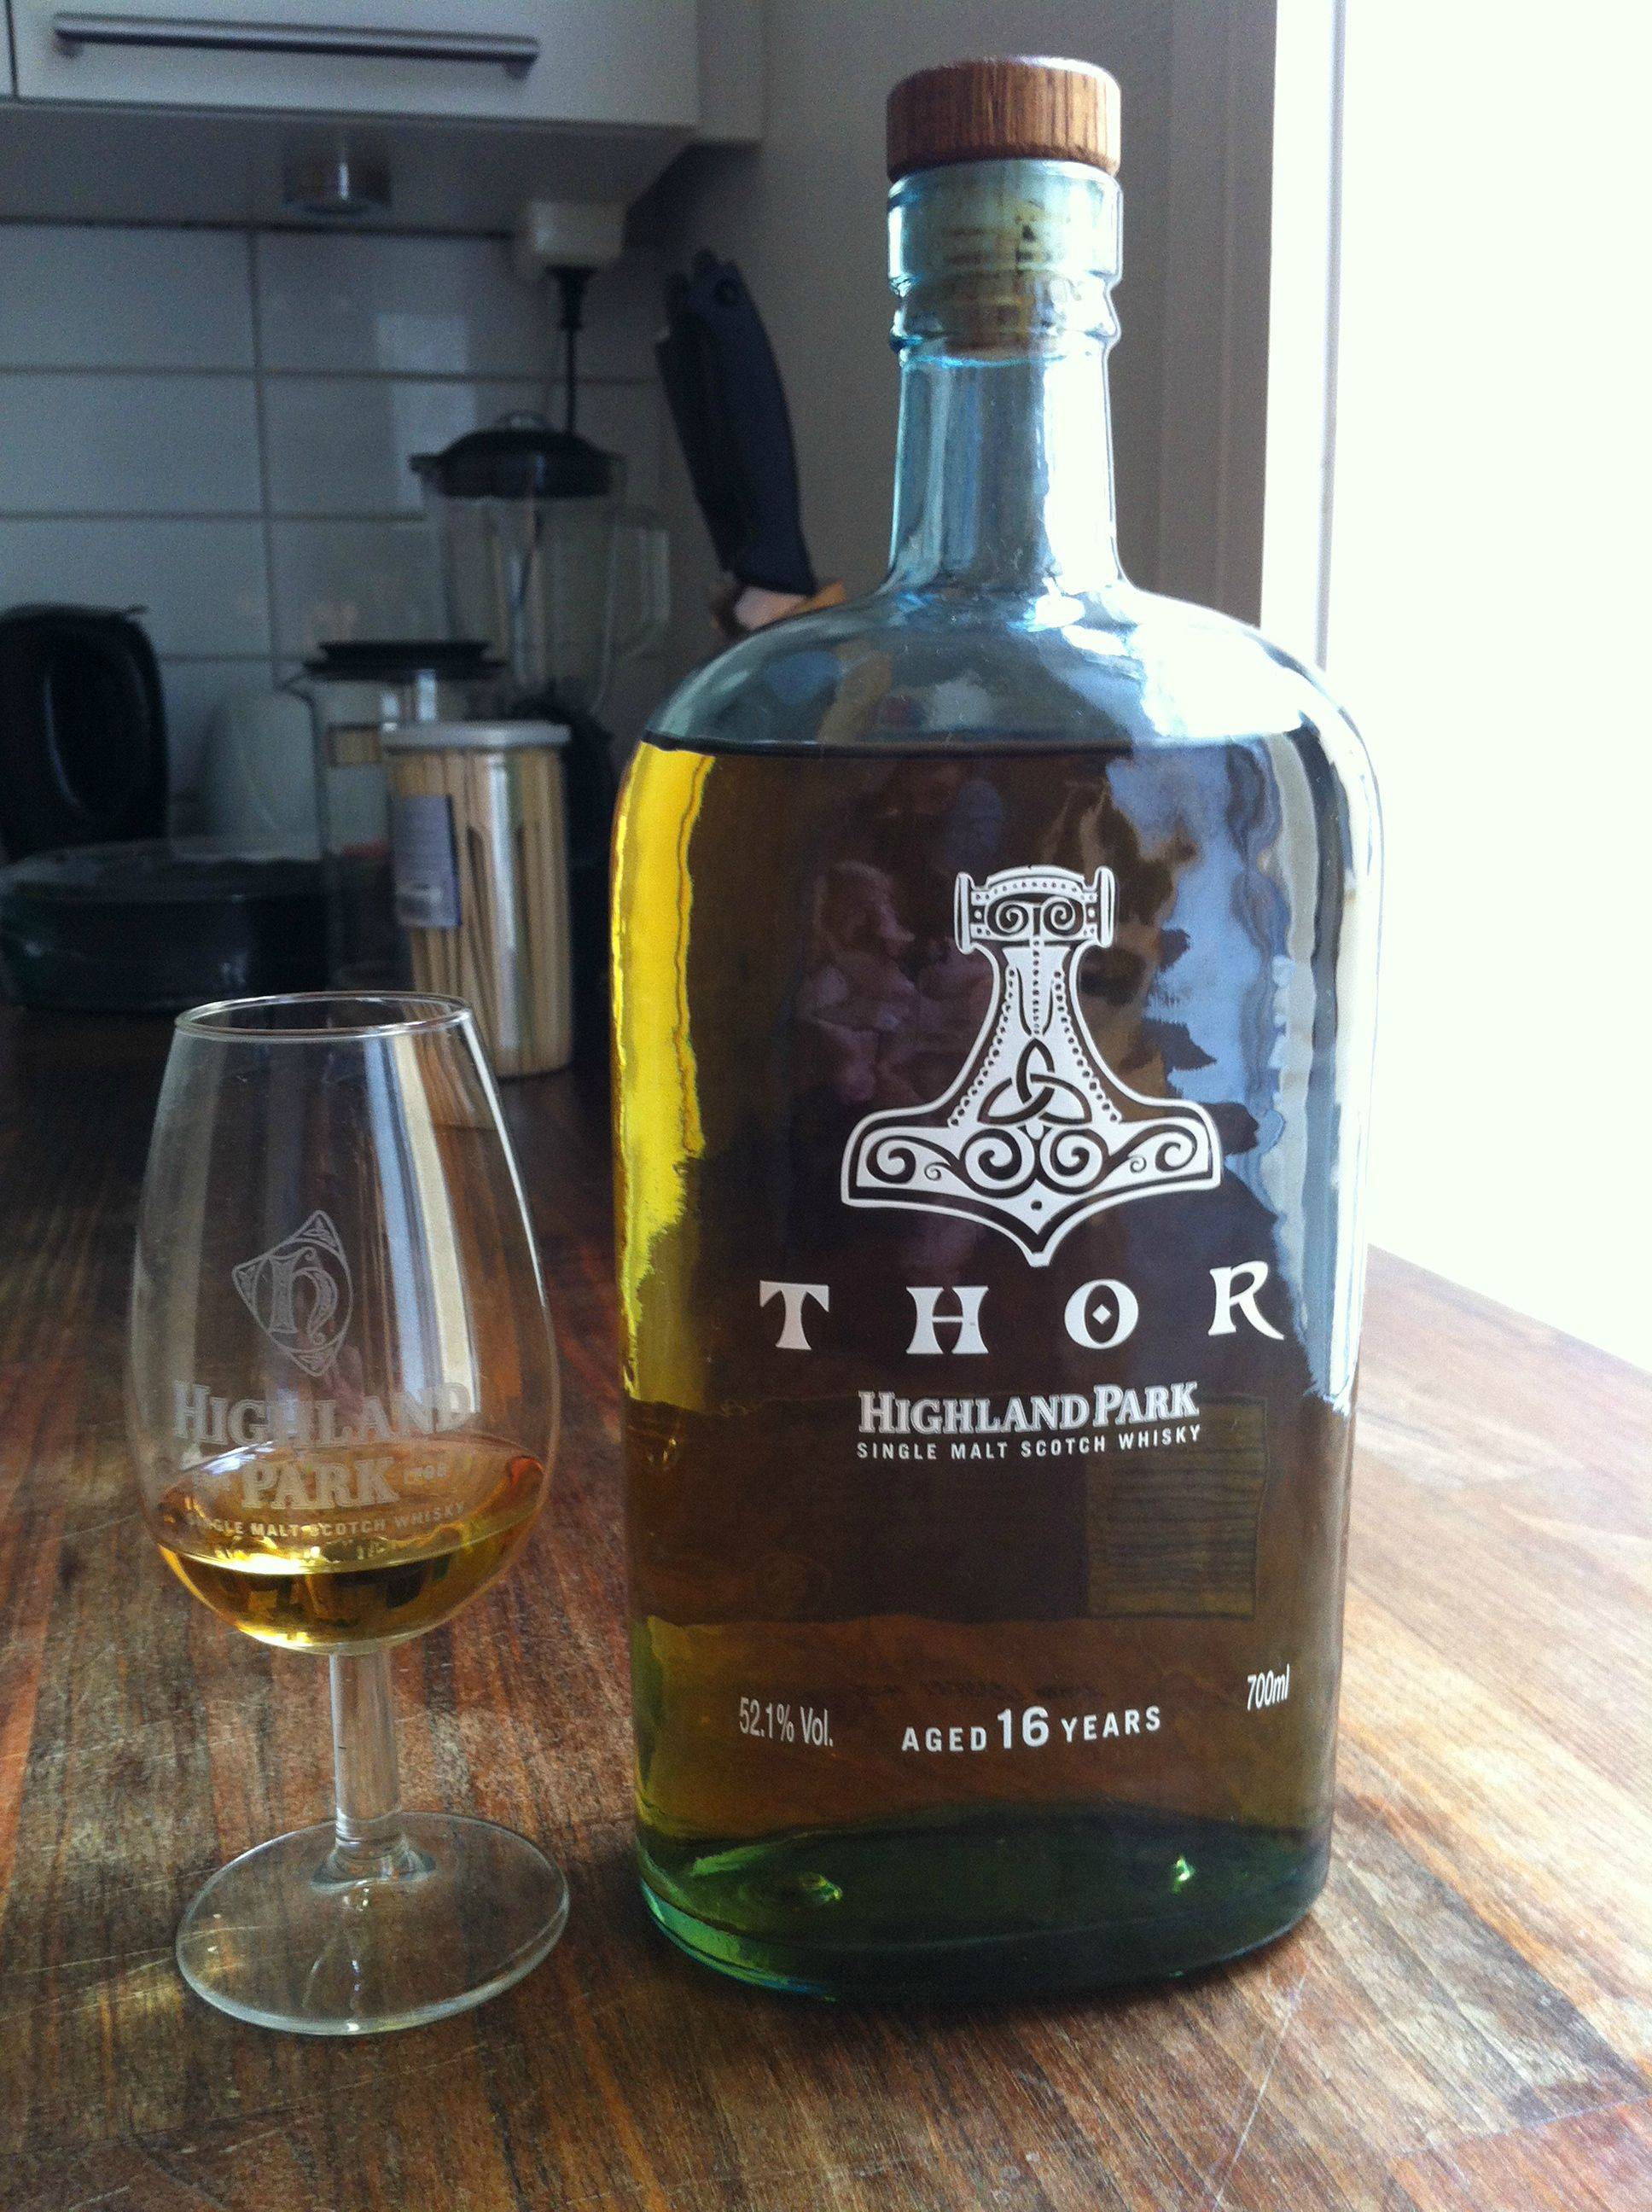
\includegraphics[scale=0.1]{Bilder/Sprit/HighlandParkThor.jpg}
\caption{Thor 16 Year fra "Highland Park"}
\end{figure}     


\newpage
\subsection{Cognac}
\end{document}